\documentclass[a4paper]{article}
\usepackage[12pt]{extsizes}
\linespread{1.5}
\usepackage[warn]{mathtext}
\usepackage[utf8]{inputenc}
\usepackage[T2A]{fontenc}
\usepackage[english,russian]{babel}
\usepackage{booktabs}
\usepackage{multicol}
\usepackage{fancyhdr}
\usepackage{graphicx}
\usepackage{microtype}
\usepackage{wrapfig}
\usepackage{amsmath}
\usepackage{floatflt}
\usepackage{geometry} 
\usepackage{float}
\usepackage{amssymb}
\usepackage{caption}
\usepackage{epsfig}
\usepackage{newunicodechar}
\usepackage{xcolor}
\usepackage{hyperref}

\usepackage{listings}
\usepackage{color}
 % Цвета для гиперссылок
 
\hypersetup{pdfstartview=FitH, colorlinks=false, pdfborder={0 0 0}}

\definecolor{dkgreen}{rgb}{0,0.6,0}
\definecolor{gray}{rgb}{0.5,0.5,0.5}
\definecolor{mauve}{rgb}{0.58,0,0.82}


\lstset{
  language=Python,
  aboveskip=1mm,
  belowskip=1mm,
  showstringspaces=false,
  columns=flexible,
  basicstyle={\small\ttfamily},
  numbers=none,
  numberstyle=\tiny\color{gray},
  keywordstyle=\color{blue},
  commentstyle=\color{dkgreen},
  stringstyle=\color{mauve},
  breaklines=true,
  breakatwhitespace=true,
  tabsize=3
}

\geometry{verbose,a4paper,tmargin=2cm,bmargin=2cm,lmargin=3cm,rmargin=1.5cm}


\begin{document}

\graphicspath{ {pictures/} }

\textbf{\Large{Аннотация}}

Данная работа посвящена определению параметров СИС-смесителя на промежуточной частоте, а именно определению уровня отражения в зависимости от напряжения смещения на смесителе. 
\par
Предлагается экспериментальная методика, которая с помощью векторного анализатора цепей позволяет найти коэффициент отражения от смесителя, когда тот находится в "рабочем" состоянии. Используется особый метод калибровки измерений, где сам СИС-переход используется как калибратор, что позволяет учесть в рассчетах его собственную емкость и индуктивность. Также предлагается проводить дополнительную калибровку по пику поглащения СИС-смесителя, так можно оценить точность расчетов, увидеть вклад комплекной части импеданса в общей коэффициент отражения и определить импеданс подводящей к СИС-переходу линии.
\par 
В результатах получено, что уровень отражений достаточно высок и варьируется от -4 до -20 дБ в зависимости от напряжения смещения смесителя. В "рабочем" состоянии отражение составляет около -5 дБ, что вынуждает использовать специальные вентили, для улучшения согласования в цепи.
\par
Теоретические рассчеты согласуются с экспериментальными данными.

\newpage
\tableofcontents
\newpage

\section{Обозначения и сокращения}

В настоящей ВКР применяются следующие сокращения и обозначения:

\begin{itemize}
    \item МФТИ	—	Московский физико-технический институт
    \item ФЭФМ	—	Физтех-школа электроники, фотоники и молекулярной физики
    \item ИРЭ	—	Институт радиотехники и электроники им. В.А. Котельникова РАН
    \item Nb	—	ниобий
    \item NbTiN	—	нитрид ниобий-титана
    \item СИС, SIS	—	туннельная структура сверхпроводник-изолятор-сверхпроводник (сосредоточенный) 
    \item РДП, FFO	—	Распределенный джозефсоновский переход (англ. flux-flow oscillator)
    \item ВАЦ, VNA — векторный анализатор цепей (англ. Vector Network Analyser)
    \item LO — опорный генератор (англ. Local Oscillator)
    \item LNA — криогенный малошумящий усилитель (англ. Low Noise Amplifier)
    \item ПЧ, IF — промежуточная частота (англ. Intermediate Frequency)
    \item ВАХ — Вольт-Амперная характеристика
\end{itemize}
\newpage


\section{Введение}

Радиоастрономия и физика атмосферы являются главными драйверами развития миллиметровых и суб-миллиметровых примеников. Данный диапазон черезвычайно информативен, однако, наименее изучен, и представляет на данный момент огромный интерес для космологии и астрофизики. В терагерцовом диапазоне отслеживают состав и стадии формирования звезд, протопланетарных систем, наблюдают детали реликтового излучения, а также изучают состав межзвездного вещества. Многие молекулы, в том числе и $H_{2}O$ имеют вращательные и колебательные спектры поглощения в субмиллиметровом диапазое.
\par

Приемники на основе смесителей на туннельном переходе сверхпроводник – изолятор – сверхпроводник (СИС) \cite{Tucker} 
имеют рекордные шумовые характеристики в диапазоне частот 100-1200 ГГц, близкие к квантовому пределу \textcolor{blue}{ссылки}.
\par

Среди СИС-приемников для наземных телескопов наибольшее распространение получили 
смесители с разделением боковых полос, которые имеют в составе два одиночных СИС-смесителя \cite{Belitsky} \cite{Chenu}. Это позволяет уменьшить вклад атмосферных шумов в два раза.

\par

Для эффективной работы 
приемника, а именно для достижения предельной чувствительности и для высокого качества разделения боковых полос, принципиально важно иметь СИС-смесители 
с низким уровнем отражения. Низкий уровень отражений нужен как по входу смесителя, т.е. на частоте принимаемого сигнала, на высокой частоте (ВЧ) 
\cite{Hesper} \cite{Khudchenko}, так и по выходу, т.е. на промежуточной частоте (ПЧ, IF). В тракте ПЧ такая необходимость обусловлена возникновением 
стоячих волн между самим СИС-смесителем и криогенным малошумящим усилителем, так как последний имеет достаточно высокий уровень отражения до $\sim -6$ дБ.
Стоячие волны увеличивают шумовую температуру и ухудшают качество разделения полос. В случае же матричных примемников важна компактность и нет возможности использовать вентили для устранения стоячих волн, поэтому минимизация отражений по ПЧ важна и для этого технического направления.
\par

Данная работа посвящена определению уровня отражений от 
СИС-смесителя в рабочем режиме с целью минимизации этого уровня в будущем. Для решения поставленной задачи проведен теоретический расчет уровня 
отражения от СИС-смесителя по выходному тракту ПЧ, а также собрана экспериментальная схема, и проведено непосредственное измерение отраженного сигнала.
\par

Полученные результаты могут быть применимы для лучшей характеризации СИС-смесителей и оптимизации их работы.


\newpage
\section{Обзор литературы}

\subsection{СИС-смеситель}

СИС-смеситель представляет собой непосредственно сам туннельный СИС-переход с выходом на применую антенную, криогенный малошумящий усилитель (LNA) и опорный генератор гетеродина (LO) (рис. \ref{fig:scheme2})

\begin{figure}[H]
    \centering
    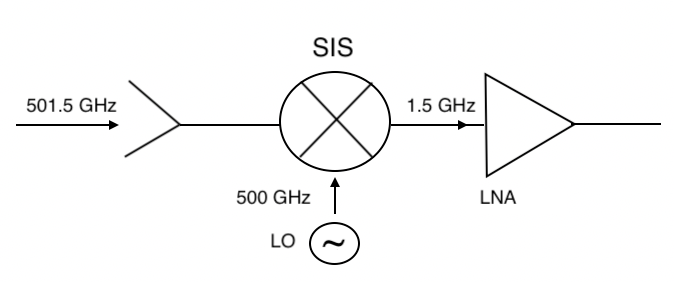
\includegraphics[scale=0.8]{scheme2.png}
    \caption{Схема СИС-смесителя}
    \label{fig:scheme2}
\end{figure}

На рис. \ref{fig:hd32} представлена интегральная согласующая структура, которая распологается полностью на одном чипе, включая СИС-переход, трансформаторы импеданса и опорный генератор на основе РДП.

\begin{figure}[H]
    \centering
    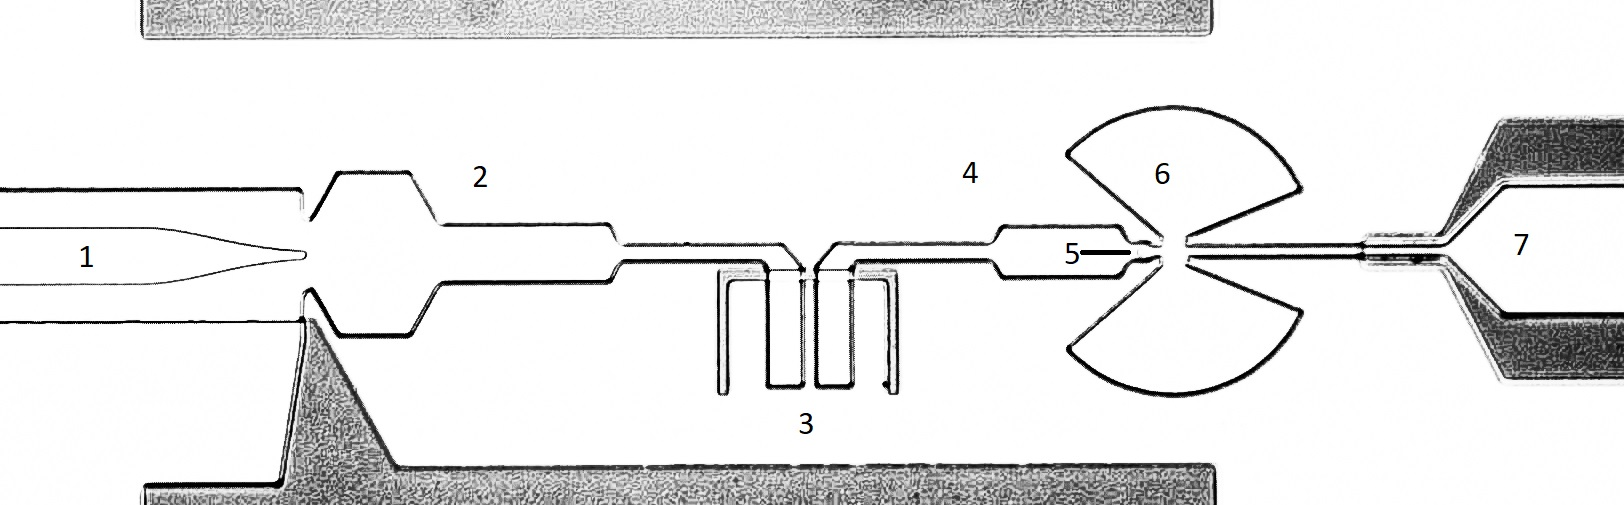
\includegraphics[scale=0.4]{HD32.jpg}
    \caption{Фото интегральной согласующей структуры. 1 — генератор на РДП, 2 — трёхступенчатый трансформатор импеданса, 3 — элемент разрыва по низким частотам, 4 — двухступенчатый трансформатор импеданса, 5 — СИС-переход, 6 — радиальный замыкатель, 7 — выходная копланарная линия.}
    \label{fig:hd32}
\end{figure}

На рис. \ref{fig:mixer} представлена конструкция <<боевого>> СИС-смесителя. Для данной конструкции внешний сигнал опорного генератора подводится через рупор.

\begin{figure}[H]
    \centering
    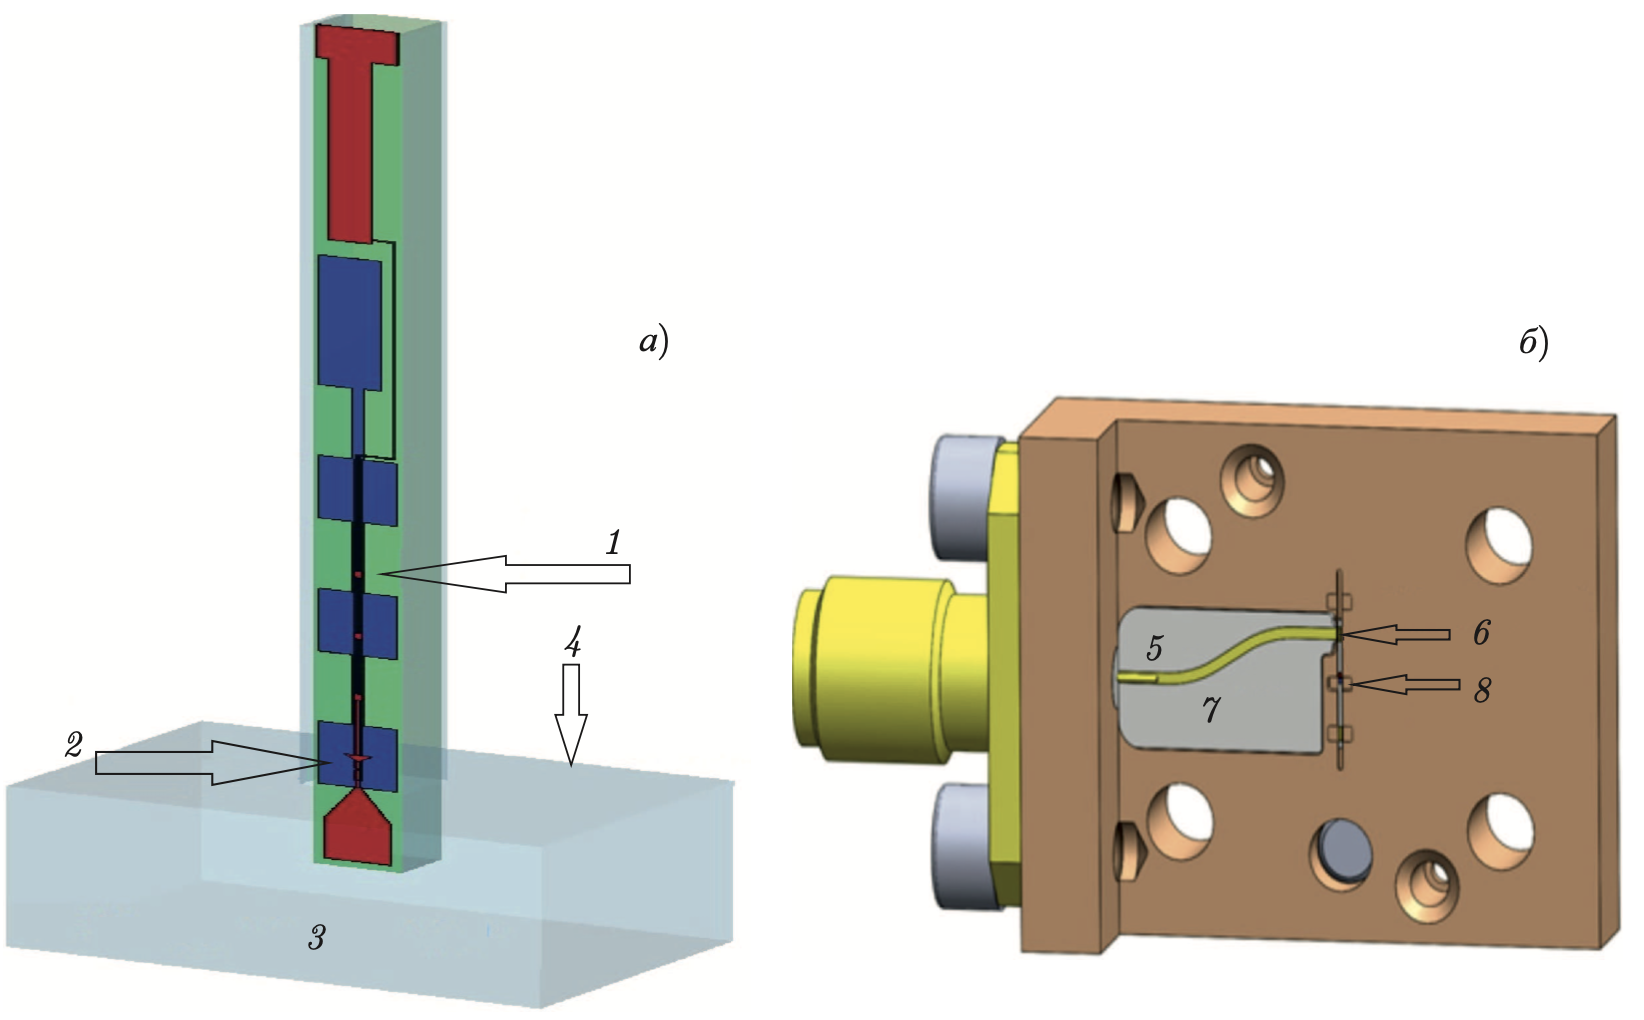
\includegraphics[scale=0.4]{mixer.png}
    \caption{\cite{Rudakov} Конструкция смесительного элемента и центральной части блока смесителя: Панель a : трёх- мерная модель дизайна смесительного элемента с размерами 3 250 × 150 × 125 мкм, размещённого в волноводе, 1 — фильтр высоких частот (ВЧ), 2 — СИС-переход, 3 — вход волновода, показа- но также расположение замыкающей стенки 4. Панель б : трёхмерная модель части смесительного блока с платой согласования по промежуточной частоте 5. В блоке установлен смесительный элемент 6, за которым в волноводе находится замыкающая плоскость; 7 — линия 50 Ом, 8 — сечение волновода, также показана область подключения волновода.}
    \label{fig:mixer}
\end{figure}

Сам туннельный СИС-переход является <<сэндвич>> структурой сверхпроводник-изолятор-сверхпроводник (рис. \ref{fig:e-diagram}). При приложении отрицательного напряжения на левый берег, энергия электронов увеличивается и будет наблюдаться туннельный ток (синяя автономная ВАХ рис. \ref{fig:e-steps}). Если при этом подать сигнал опорного генератора (LO), то энергия фотона $\hbar \omega$ позволит электронам туннелировать компенсируя недостаток энергии и образуются так называемые ступени $\hbar \omega / e$ (красная "рабочая" ВАХ рис. \ref{fig:e-steps})

\begin{figure}[H]
    \centering
    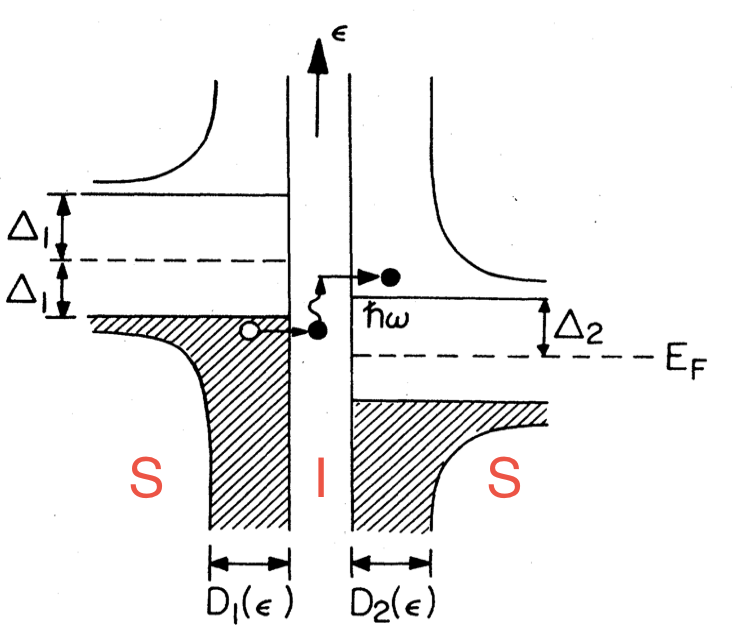
\includegraphics[scale=0.8]{e-diagram.png}
    \caption{Энергетическая диаграмма СИС-перехода \cite{Tucker}}
    \label{fig:e-diagram}
\end{figure}

\begin{figure}[H]
    \centering
    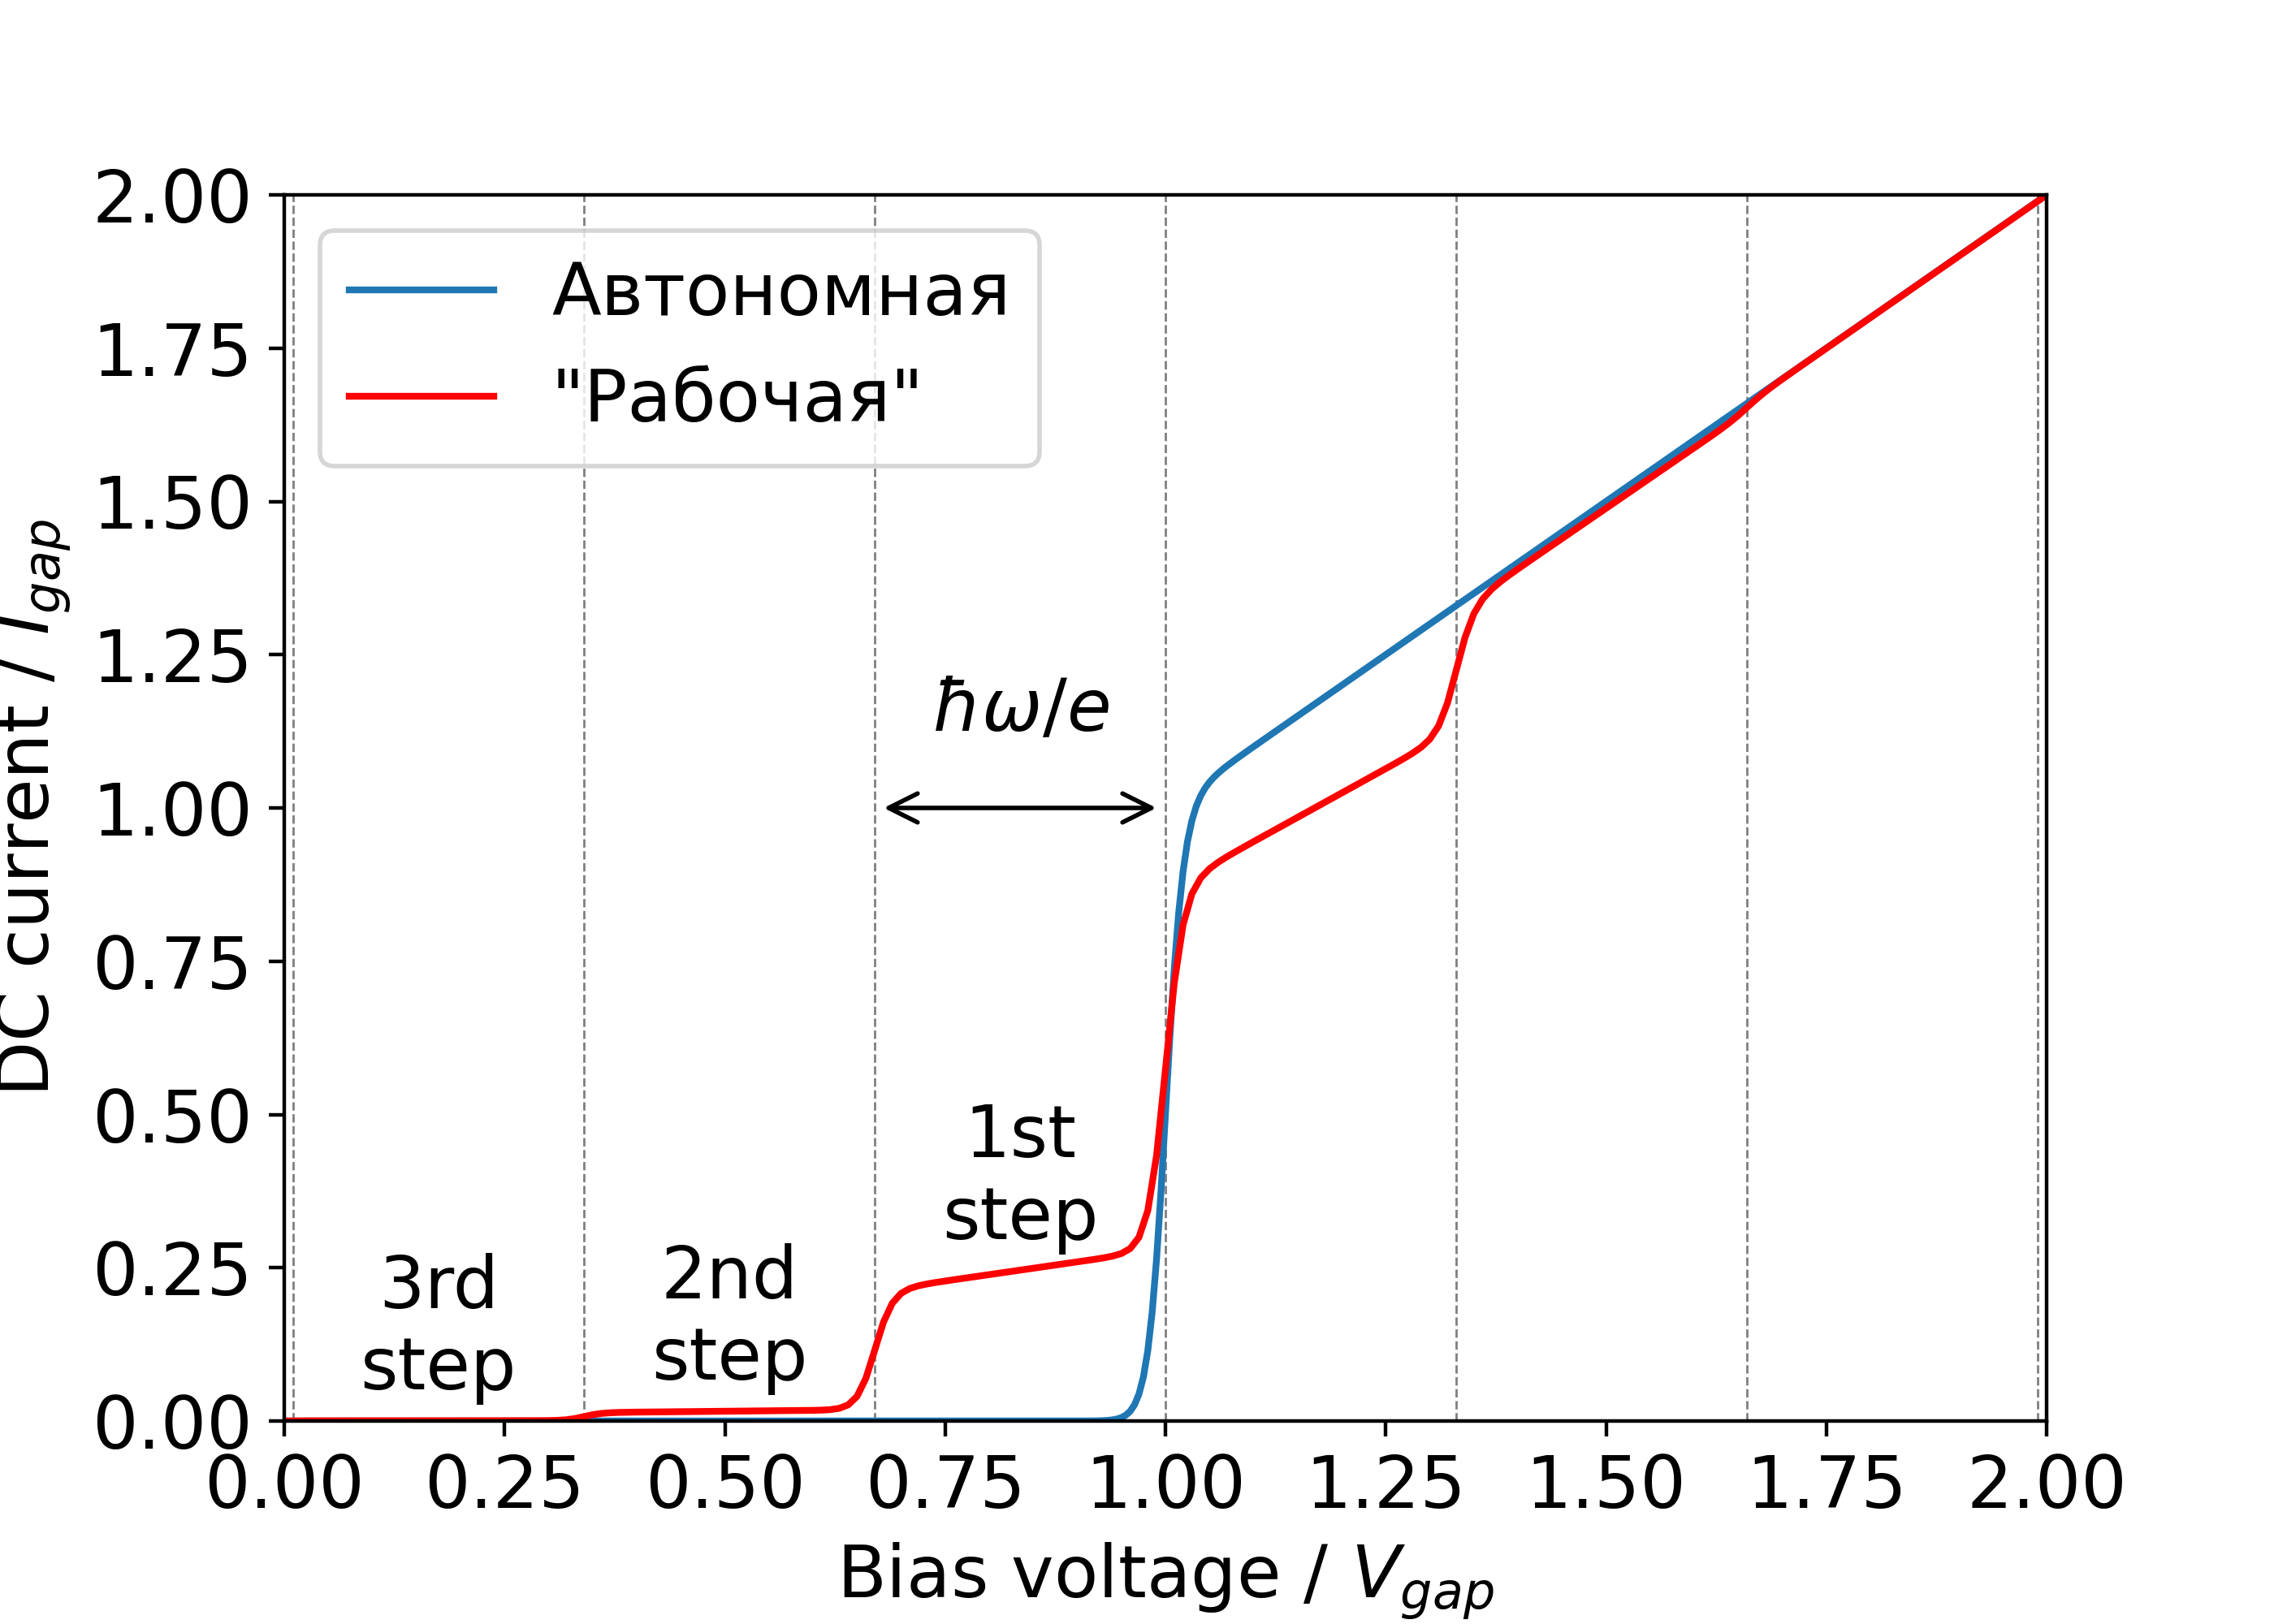
\includegraphics[scale=0.5]{steps.png}
    \caption{Теоретическая ВАХ СИС-перехода; Автономная (синяя кривая) и "Рабочая" (красная кривая) при поданном напряжении опорного генератора LO. Расчет выполнен с помощью python-библиотеки \href{https://github.com/garrettj403/QMix}{QMix}} \cite{Garrett}.
    \label{fig:e-steps}
\end{figure}

\subsection{Гетеродинный прием}

Принцип гетеродинирования \cite{Barichev} заключается в складывании мощного сигнала опорного генератора и слабого детектируемого сигнала в смесителе с нелинейной ВАХ. Ввиду нелинейности возникают суммы и разности соответсвующих частот:

\begin{equation}
    |n\cdot f_S - m \cdot f_{LO}|
\end{equation}

где $f_S$ — частота слабого детектируемого сигнала, $f_{LO}$ — частота мощного сигнала опорного генератора.

Для примера, возьмем квадратичную ВАХ: $I(V) \sim V^2$. Сигналы принимаемый и опорного генератора соответсвенно:

\begin{equation}
    V_S = V_S \sin(2\pi f_S t); \;\;  V_{LO} = V_{LO} \sin(2\pi f_{LO} t)
\end{equation}

Тогда ток смесителя при приложеных сигналах и напряжении смещения $V_0$:
\begin{equation}
    \begin{split}
       I \sim \left ( V_0 +  V_{LO} \sin(2\pi f_{LO} t) + V_S \sin(2\pi f_S t)  \right )^2 \\
       \sim V_0^2 + 2V_0V_S \sin(2\pi f_S t) + 2V_0V_{LO} \sin(2\pi f_{LO}t) \\
        + \frac{1}{2} V_S^2 \left \{ 1 - \cos(2\pi (2f_S)t) \right \}
        + \frac{1}{2} V_{LO}^2 \left \{ 1 - \cos[2\pi (2f_{LO})t] \right \} \\
        + V_S V_{LO} \left \{ \cos(2\pi (f_S - f_{LO})t) - \cos(2\pi (f_S + f_{LO})t) \right \}
    \end{split}
\end{equation}

Итак, мы можем выделить компоненту сигнала $V_S V_{LO} \cos(2\pi(f_S - f_{LO}) t)$. Эта разностная частота называется промежуточной частотой (ПЧ) $f_0$:

\begin{equation}
    f_S = f_{LO} \pm f_0
\end{equation}

Таким образом гетеродин позволяет "сбросить" частоту принимаемого сигнала $f_S$ до промежуточной частоты $f_0$, сохраняя пропорции величины сигнала. На рис. \ref{fig:heterodyne} проиллюстрирован принцип "сброса" частоты гетеродином.

\begin{figure}[H]
    \centering
    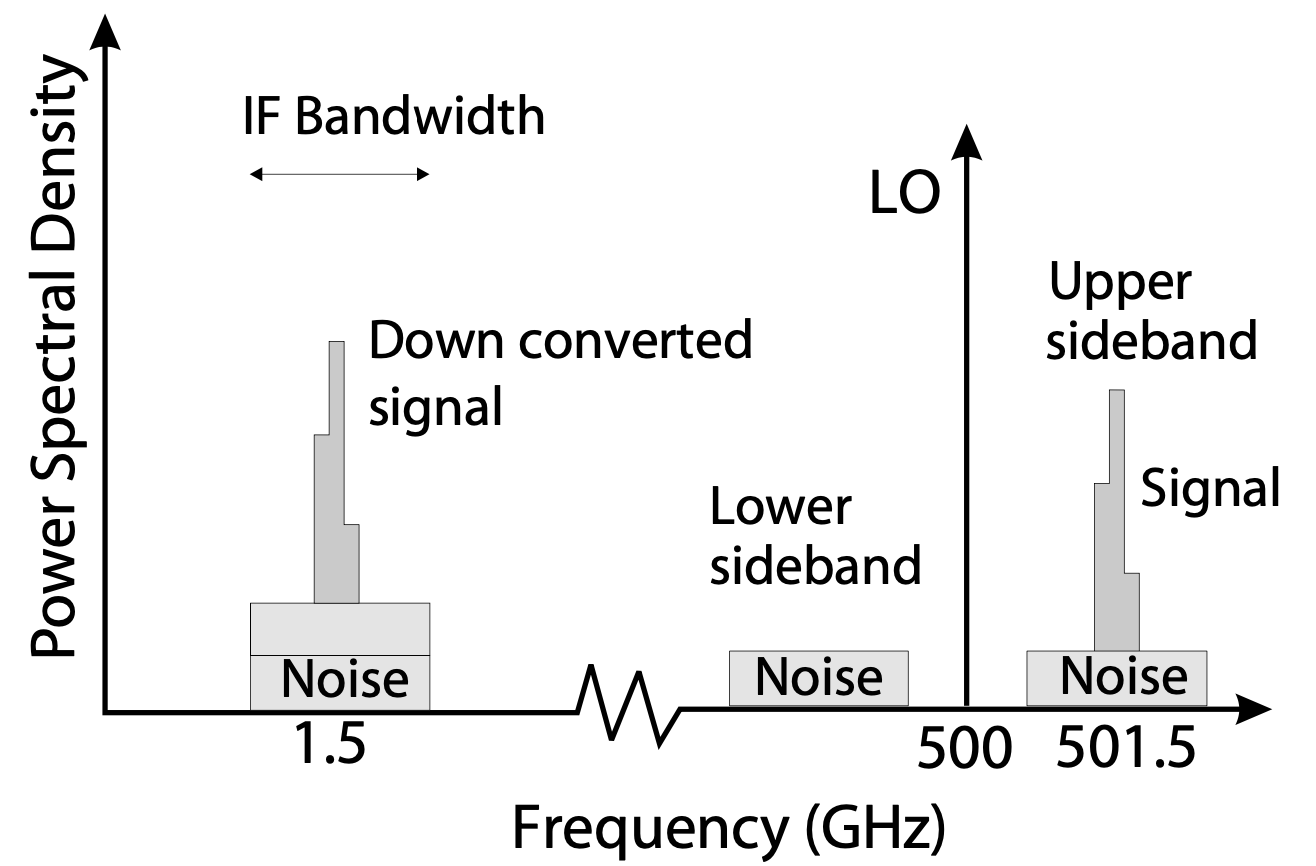
\includegraphics[scale=0.5]{heterodyne.png}
    \caption{Иллюстрация принципа гетеродинирования \cite{Barichev}. Детектируемый сигнал частоты $f_S = 501.5\; GHz$, сигнал LO  $f_{LO} = 500 \; GHz$, сигнал ПЧ $f_0 = 1.5 \; GHz$.}
    \label{fig:heterodyne}
\end{figure}


\subsection{Измерение отражений от СИС-смесителя}

На данный момент достаточно много научных статей, посвященных изучению криогенных приемников на основе туннельного перехода СИС и их различных характеристик[ссылки].
Однако, вопрос непосредственного измерения уровня отражения от СИС-смесителя на промежуточной частоте затрагивает лишь несколько работ:
\par

\begin{itemize}
    \item В работе Serres et al. \cite{Serres}, посвященной определению выходного импеданса СИС-смесителя по        промежуточной частоте, приведено сравнение теоретических 
        рассчетов и экспериментальных результатов. Цель данной статьи достаточно близка к нашей, поскольку определение импеданса необходимо для получения уровня отражения.
        Предложена модифицировання однопортовая экспериментальная схема с использованием циркулятора (рис. \ref{fig:serres-scheme}).
        \begin{figure}[H]
            \centering
            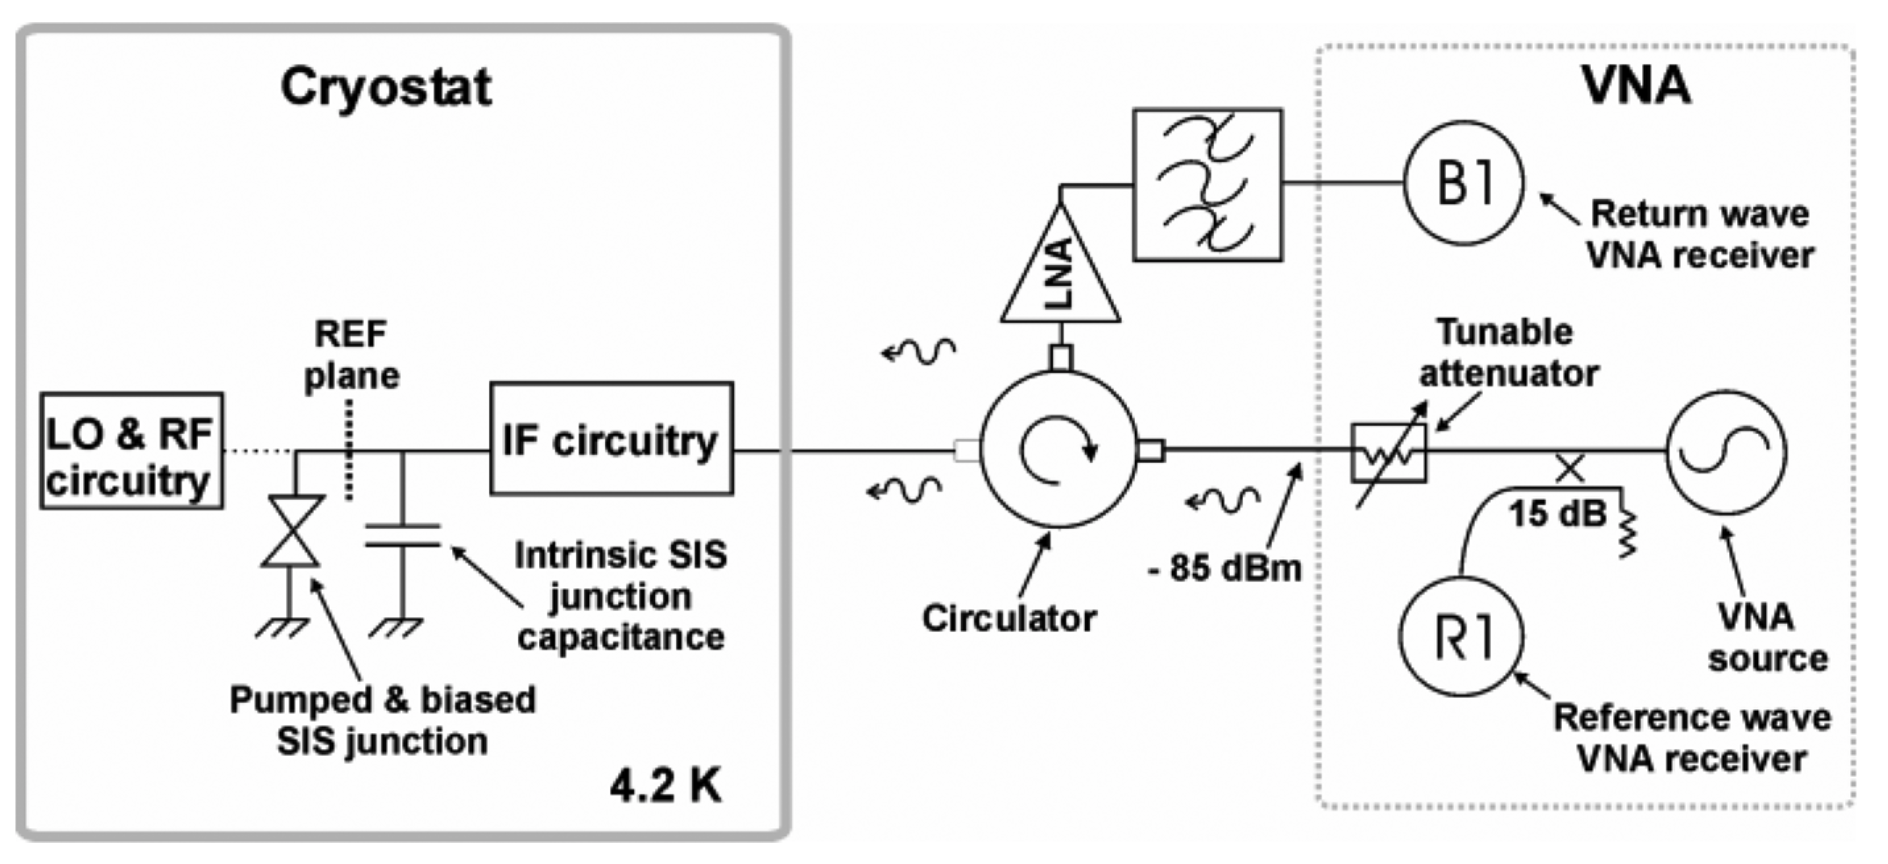
\includegraphics[scale=0.45]{serres-scheme.png}
            \caption{Система измерения импеданса ПЧ СИС-смесителя с модифицированной конфигурацией однопортового ВАЦ. Криостат и ВАЦ показаны соответственно слева и справа. Посередине показаны направления падающей и обратной волн от ВАЦ, а также соединения циркулятора с криостатом и ВАЦ. Криостат содержит СИС-смеситель с его схемой ПЧ, а также внешние коаксиальные кабели инжектора Bias-Tee и ПЧ, которые соединяют выход ПЧ смесителя с пластиной криостата 300 К. \cite{Serres}}
            \label{fig:serres-scheme}
        \end{figure}
        Особенностью калибровки является то, что сам СИС-сместель используется как калибратор, двигаясь по его вольт-амперной характеристике (ВАХ) можно получить три калибрововчных стандарта (SOL).\par
        Причем, такая калибровка позволяет учесть собственную емкость и индуктивность перехода.
        Численный рассчет импеданса смесителя в данной работе опирается на теорию Tucker et al. \cite{Tucker}.
        \par
        Особенности: все в холоде, размеры маленькие
        \par
    \item В кандидатской диссертации (PhD thesis) А.М. Барышева (Barichev A.M) \cite{Barichev} приводится пример распростроненной схемы для измерения отражений от СИС-смесителя по тракту     ПЧ (рис. \ref{fig:barichev}), на который мы будем ориентироваться при составлении схемы нашего экспримента.
        \begin{figure}[H]
            \centering
            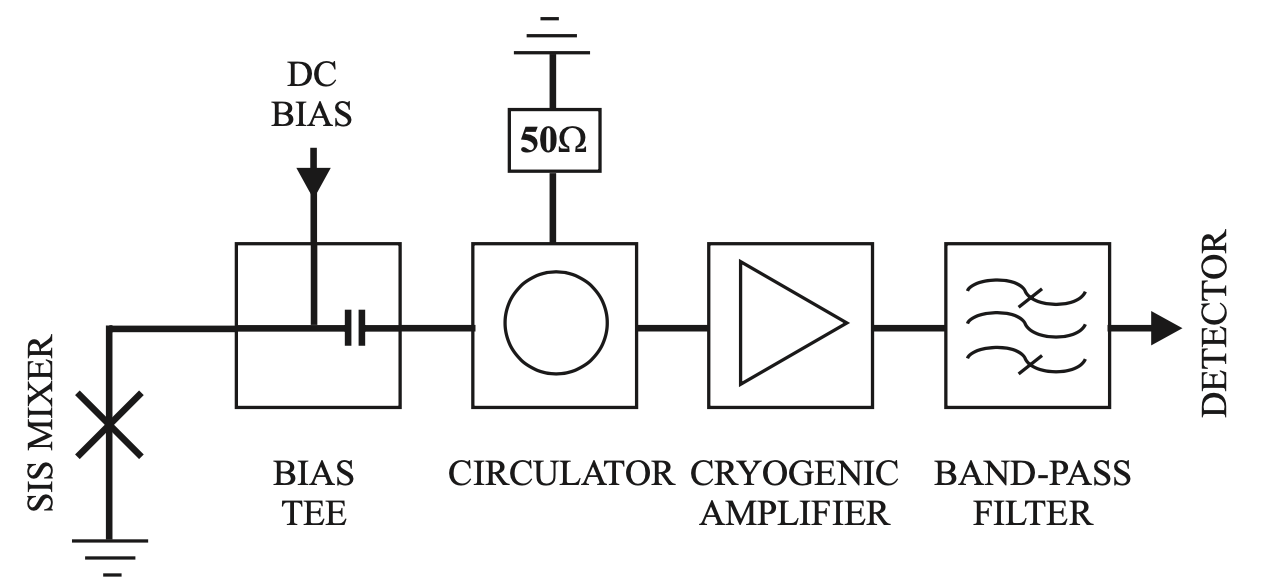
\includegraphics[scale=0.5]{barichev.png}
            \caption{Типичная схема соединения СИС-смесителя по выходу ПЧ \cite{Barichev}}
            \label{fig:barichev}
        \end{figure}
\end{itemize}

\section{Расчет и измерение отражения}

\subsection{Схема эксперимента}

Основная задача данной работы заключается в измерении уровня отражения от СИС-смесителя по выходному каналу ПЧ, когда сам смеситель находится в рабочем состоянии, а именно на него подается напряжение смещения и приложен сигнал высокочастотного опорного генератора. 

Измерение отражений от СИС-смеситея имеет ряд принципиальных особенностей:
\begin{itemize}
    \item СИС-смеситель насыщается сигналом малой мощности, что вызывает искажение ВАХ и искажает режим его работы, поэтому уровень тестового сигнала VNA, приходящего на СИС по тракту ПЧ, не должна превышать -50дБм. 
    \item отраженный от СИС-смеситея сигнал очень мал и должен быть усилен с помощью МШУ перед подачей на ВАЦ
    \item СИС-смеситель расположен в криостате при температуре 4К, а ВАЦ при комнатной тетмпературе
    
\end{itemize}

Измерения проведены в диапазоне 4–8 ГГц; этот диапазон определен полосой используемого криогенного ПЧ усилителя. Схема эксперимента представлена на Рис.\ref{pic-setup}; 
СИС-смеситель помещен в криостат замкнутого цикла при температуре около 4 K. Высокочастотный опорный генератор (LO) интегрирован с СИС-смесителем на одном 
чипе и представляет собой распределенный джозефсоновский переход c вязким течением магнитных вихрей (РДП, FFO).  Векторный анализатор цепей (ВАЦ, VNA), 
размещенный вне криостата, генерирует тестовый сигнал диапазона 4–8 ГГц на порте (П1, P1), который, проходя через аттенюатор -10 дБ, поступает в направленный 
ответвитель (Directional coupler), который направляет его на СИС-смеситель с коэффициентом связи около -10 дБ. Далее сигнал проходит специальный инжектор (Bias Tee), 
позволяющий беспрепятственно проходить ПЧ сигналу, задавая при этом напряжение на СИС-смесителе по постоянному току через большую индуктивность. 
Отразившись от СИС-смесителя, основная часть сигнала проходит напрямую через направленный ответвитель и поступает на вход криогенного малошумящего усилителя (LNA), 
который усиливает этот сигнал и направляет его на приемный порт (П2, P2) ВАЦ. Фактически, измеряемым параметром является отношение сигналов ВАЦ на портах П1 и П2, а точнее его спектр.

\begin{figure}[H]
    \begin{center}
        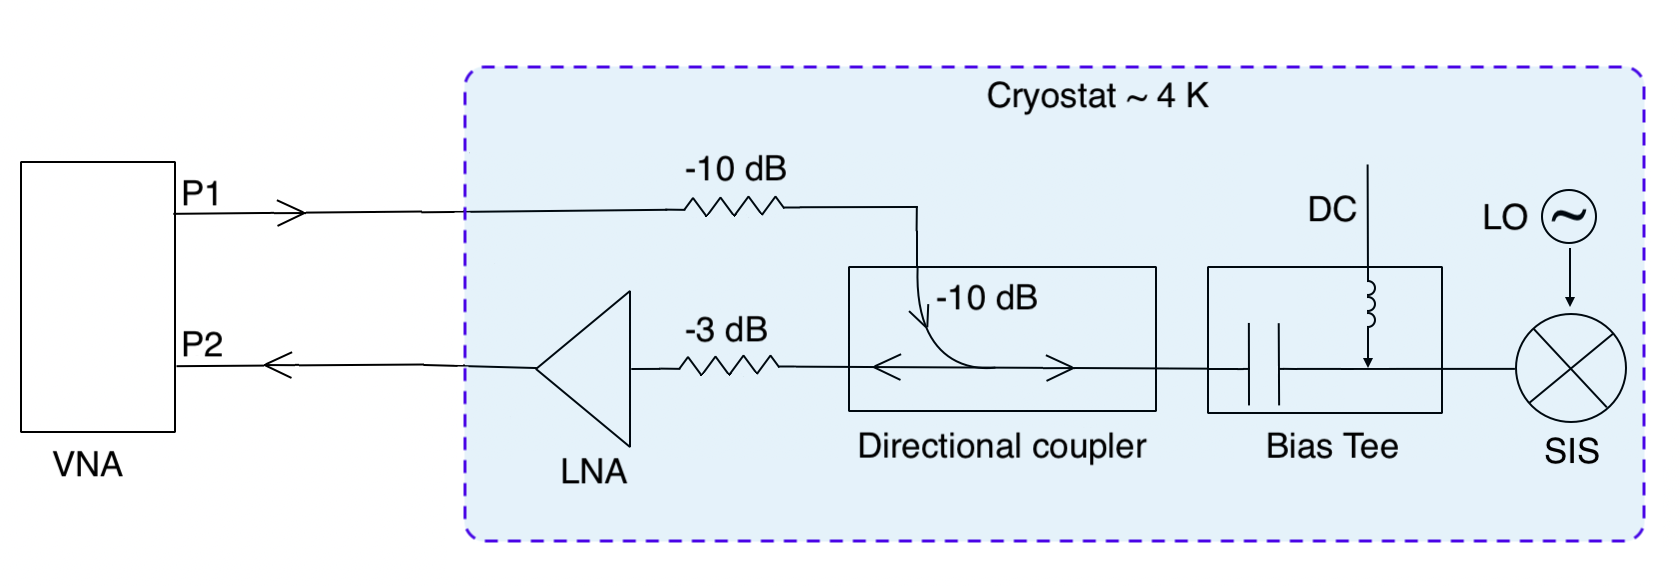
\includegraphics[scale=0.5]{setup.png}
        \caption{Схема эксперимента по измерению отражения от СИС-смесителя по выходу ПЧ}
        \label{pic-setup}
    \end{center}
\end{figure}

Ниже представлены фото собранных измерительных установок (рис. \ref{fig:exp_photo1} и \ref{fig:exp_photo} соответственно) с использованием интегральной согласующей структуры (схема на рис. \ref{fig:hd32}) и волноводного СИС-смесителя диапазона 211-275 ГГц (схема на рис. \ref{fig:mixer}).

\begin{figure}[H]
    \begin{center}
        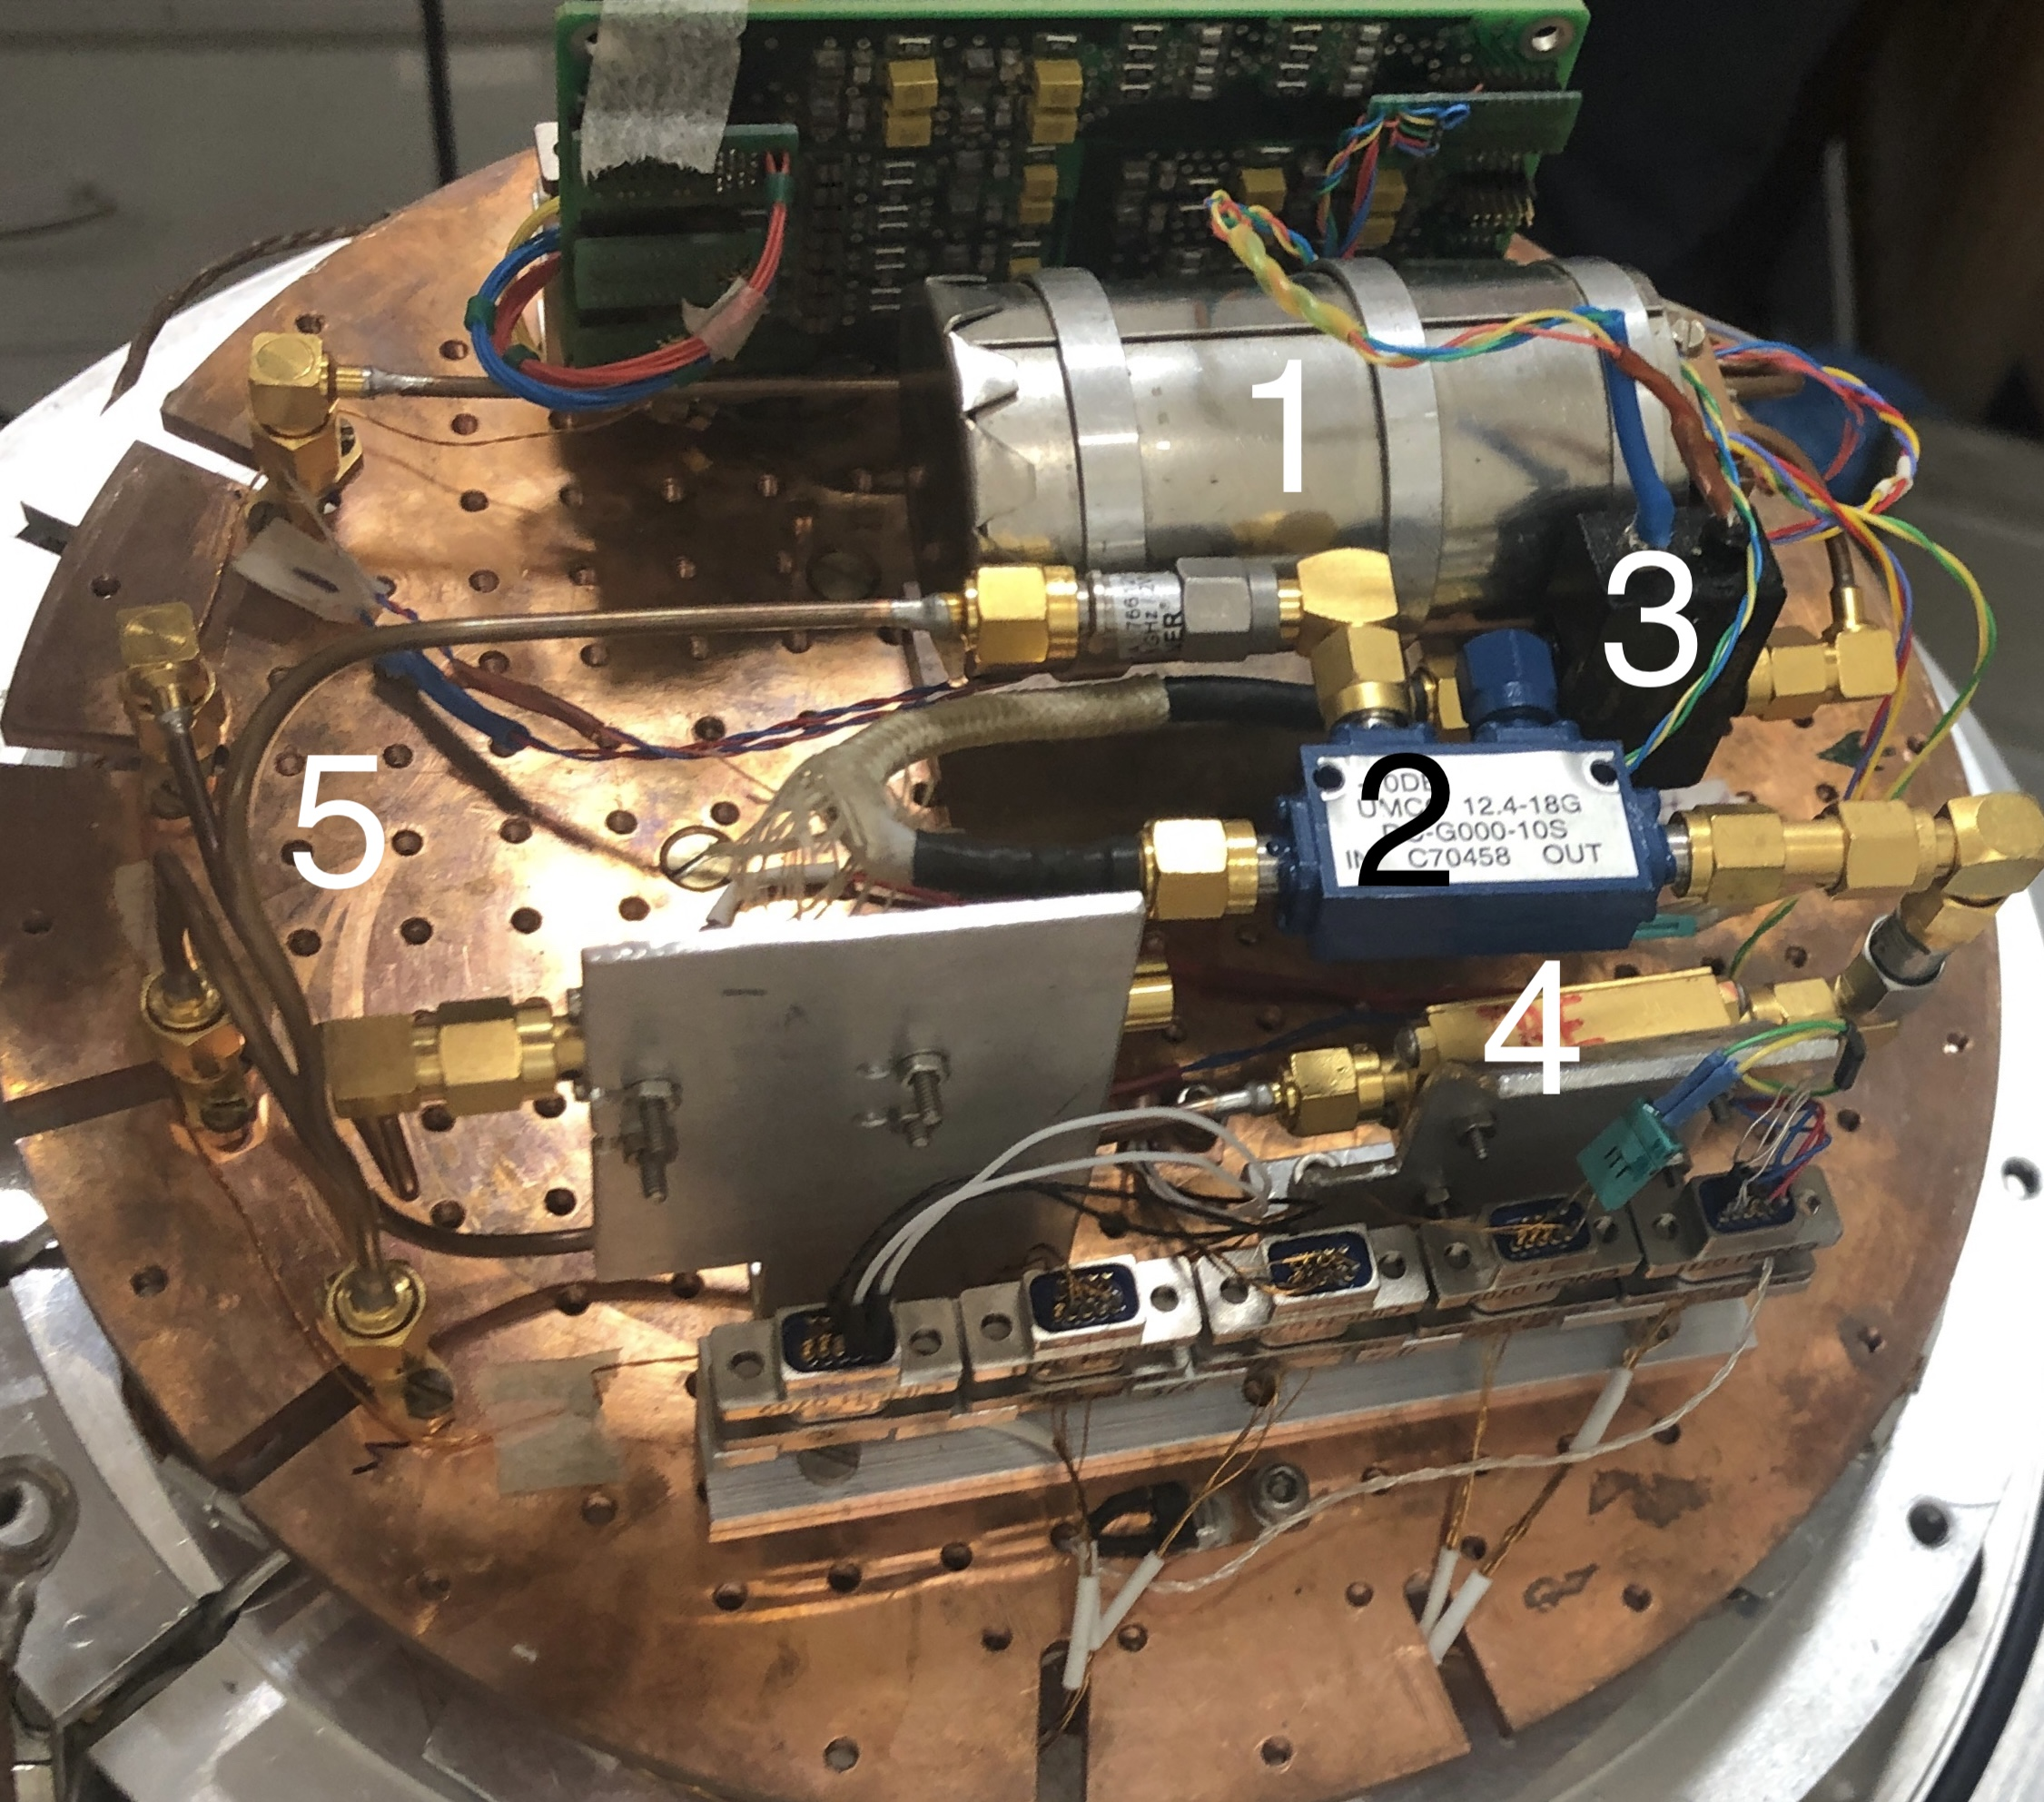
\includegraphics[scale=0.1]{exp_photo1.jpg}
        \caption{Фото установки внутри криостата при измерении отражения от интегрального СИС-смесителя. 1 — Металлический экран (внутри чип с интегральной согласующей структурой), 2 — Направленный ответвитель, 3 — Инжектор, 4 — криогенный усилитель, 5 — плита криостата $\sim 4\; K$.}
        \label{fig:exp_photo1}
    \end{center}
\end{figure}

\begin{figure}[H]
    \begin{center}
        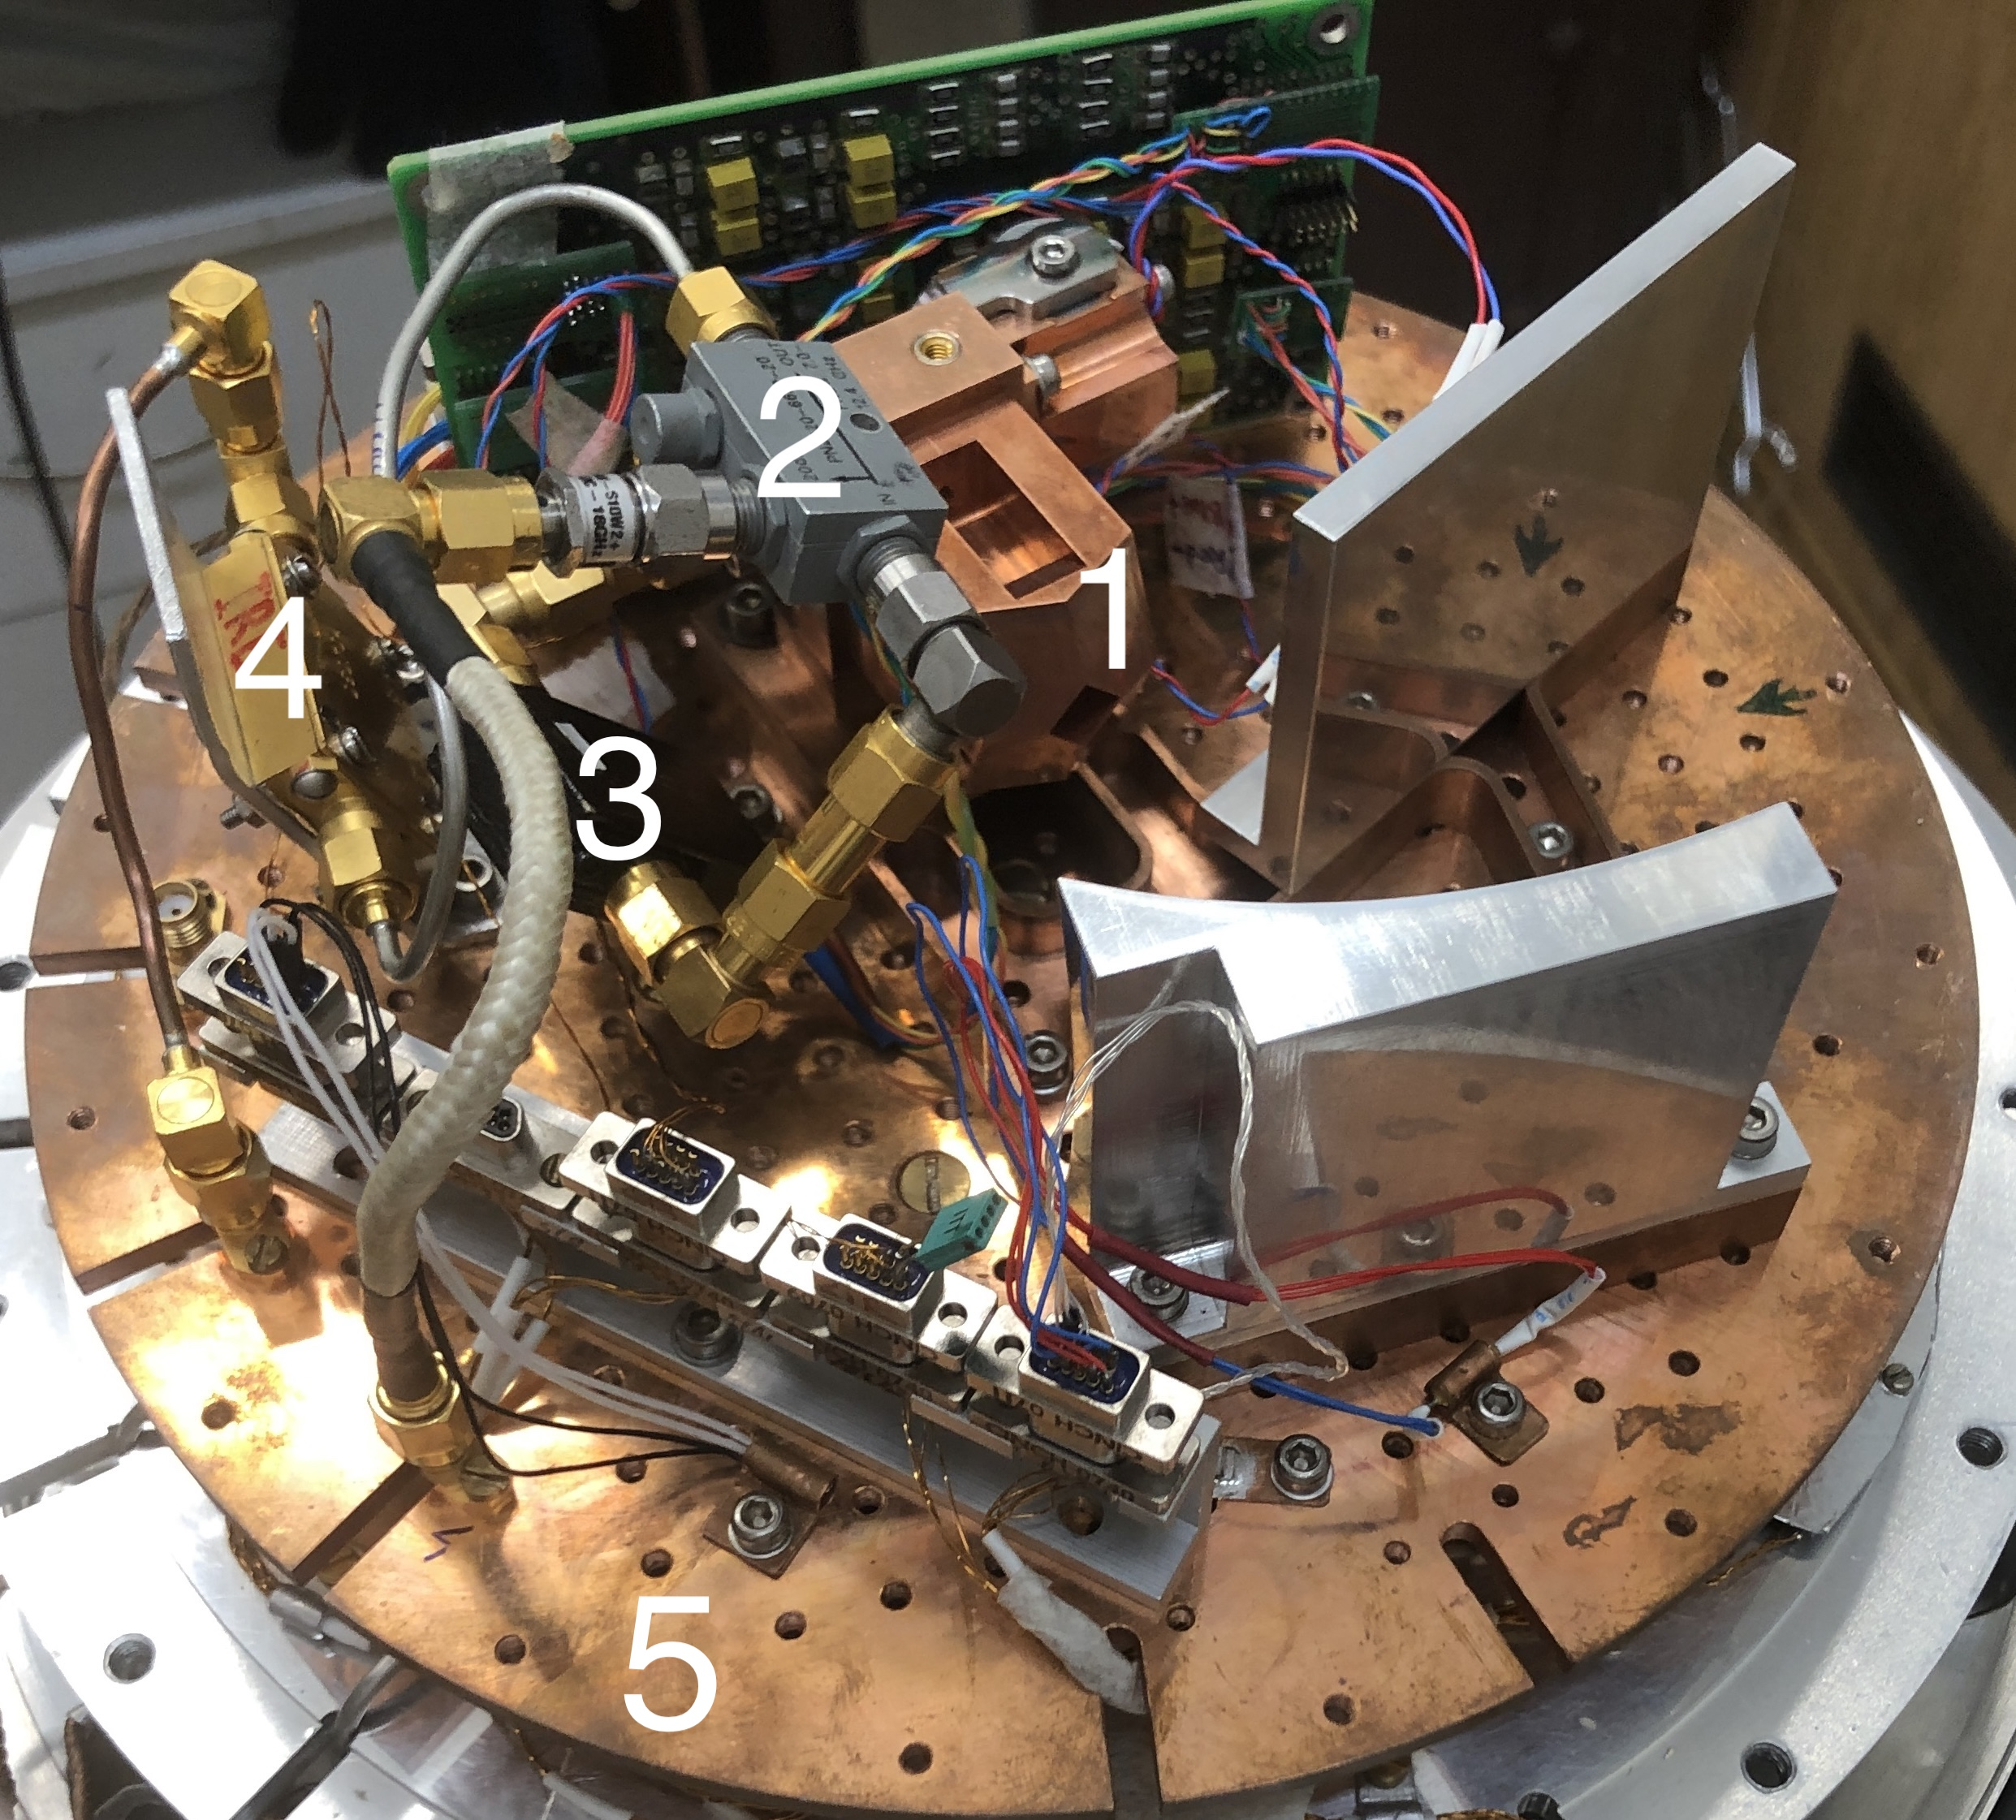
\includegraphics[scale=0.1]{exp_photo.jpg}
        \caption{Фото установки внутри криостата при измерении отражения от <<боевого>> волноводного СИС-смесителя диапазона 211-275 ГГц. 1 — Рупор СИС-приемника, 2 — Направленный ответвитель, 3 — Инжектор, 4 — криогенный усилитель, 5 — плита криостата $\sim 4\; K$.}
        \label{fig:exp_photo}
    \end{center}
\end{figure}


\subsection{Калибровка цепи}

Обязательным этапом для измерений отражения является калибровка цепи. Мы используем калибровку, эквивалентную стандартной однопортовую калибровку (Рис. \ref{pic-error}), 
в основе которой лежит определение 3х параметров цепи: D - прямые утечки в цепи, R - внутренние отражения, M - рассогласование. 

\begin{figure}[H]
    \begin{center}
        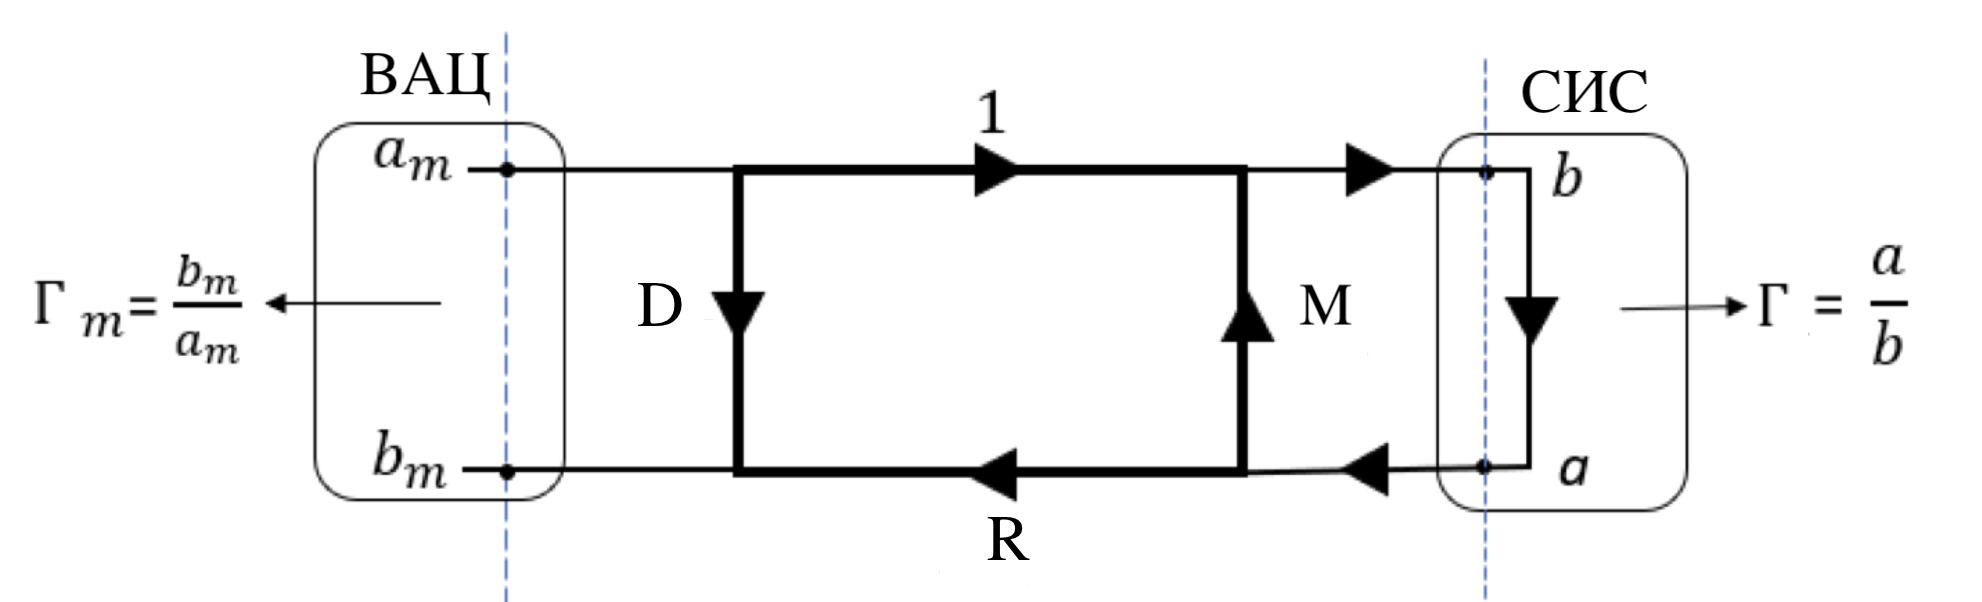
\includegraphics[scale=0.4]{Error.png}
        \caption{Схема однопортовой калибровки.}
        \label{pic-error}
    \end{center}
\end{figure}

Путем несложных преобразований (полные выкладки можно найти в \cite{Walker}), используя последовательное (рис. \ref{fig:series-rule}) и параллельное (рис. \ref{fig:parallel-rule}) правила расчета коэффициента пропускания элементов цепи можно явно выразить фактический коэффициент отражения $\Gamma$  через измеряемую величину $\Gamma_m$ и 3 калибровочных параметра D, R, M:

\begin{equation}
    \Gamma = \frac{\Gamma_m - D}{R + M(\Gamma_m - D)}
    \label{gamma}
\end{equation}

\begin{figure}[H]
    \begin{center}
        \begin{minipage}[H]{0.4\linewidth}
            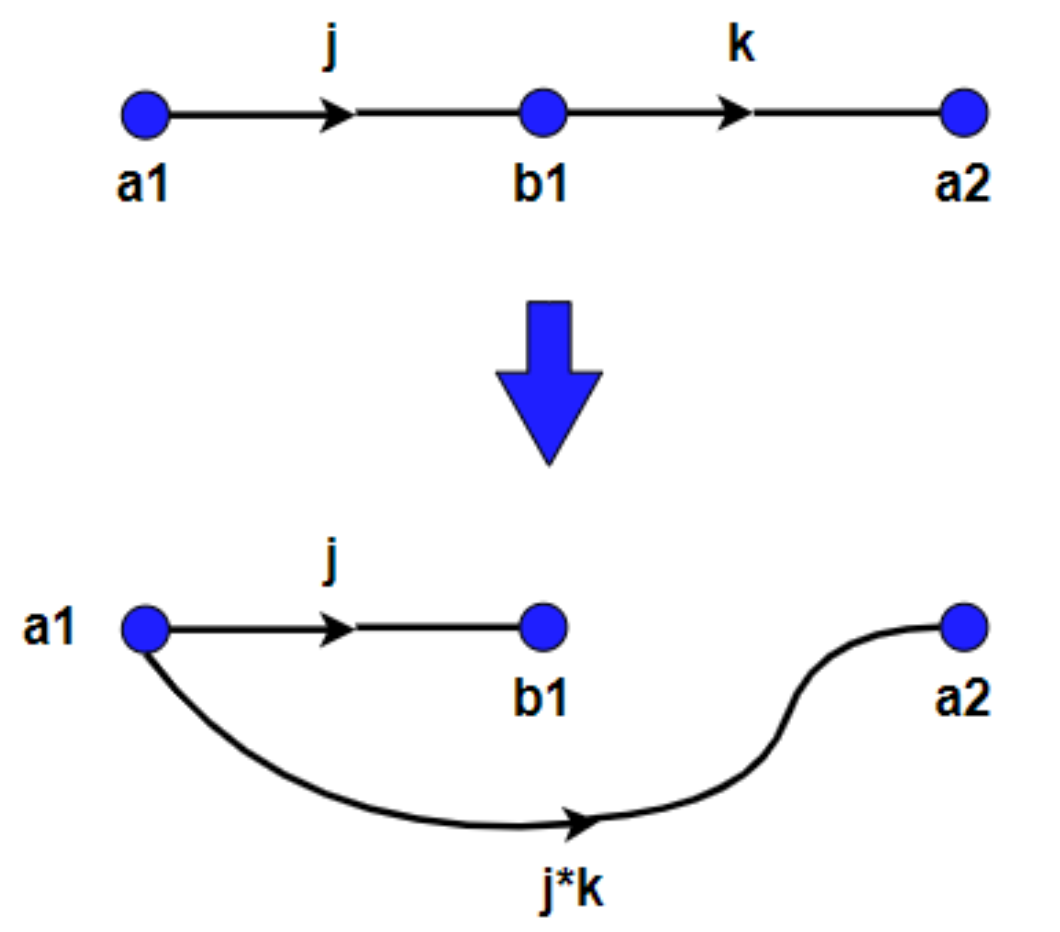
\includegraphics[width=1\linewidth]{series-rule.png}
            \caption{Последовательное правило \cite{Walker}} 
            \label{fig:series-rule}
        \end{minipage}
        \hfill 
        \begin{minipage}[H]{0.45\linewidth}
            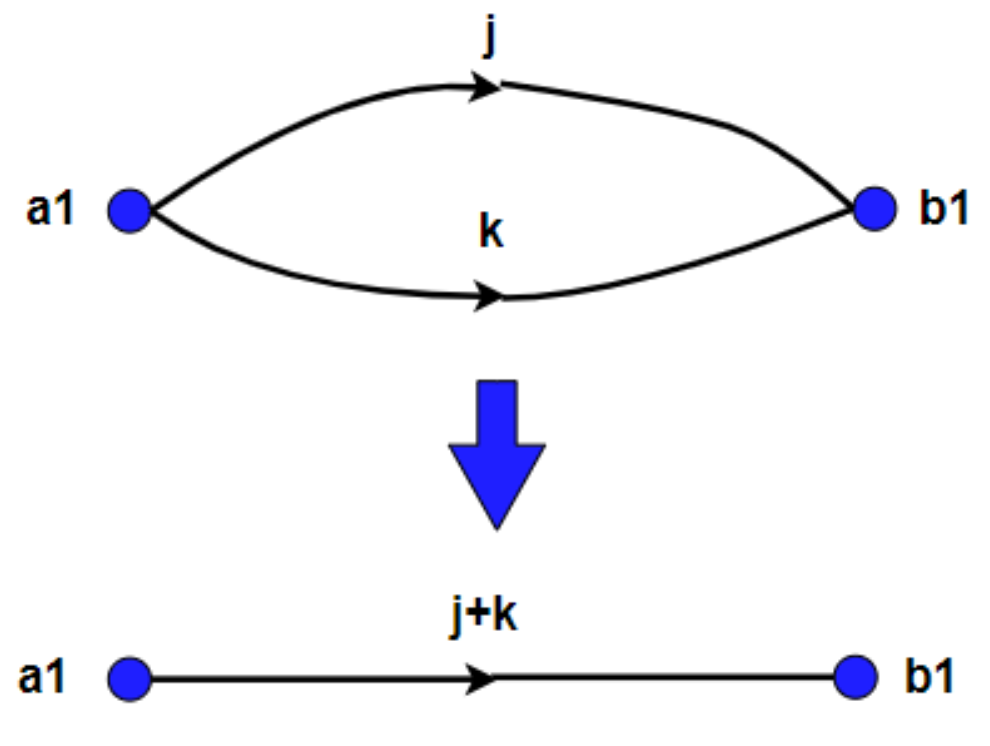
\includegraphics[width=1\linewidth]{parallel-rule.png}
            \caption{Параллельное правило \cite{Walker}}
            \label{fig:parallel-rule}
        \end{minipage}
    \end{center}
\end{figure}

Коэффициенты D, R, M могут быть определены по трем калибровочным измерениям, путем составления и решения системы (\ref{eq:sys}) из трех уравнений (\ref{gamma}), где коэффициент отражения  вычисляется теоретически по формуле (\ref{s11}), а величина  непосредственно измеряется векторным анализатором цепей.

\begin{equation}
    \begin{cases}
        \frac{\Gamma_{m_{open}} - D}{R + M(\Gamma_{m_{open}} - D)} = \Gamma_{open} \; \text{Открытая цепь} \\
        \frac{\Gamma_{m_{short}} - D}{R + M(\Gamma_{m_{short}} - D)} = \Gamma_{short} \; \text{Короткое замыкание}\\
        \frac{\Gamma_{m_{load}} - D}{R + M(\Gamma_{m_{load}} - D)} = \Gamma_{load} \; \text{Нагруженная линия} \\
    \end{cases}
    \label{eq:sys}
\end{equation}

Представим систему (\ref{eq:sys}) в матричном виде \cite{Walker}:

\begin{equation}
    \begin{bmatrix}
        E_1\\
        E_2\\
        E_3\\
    \end{bmatrix}
    =
    \left( C^{\dag}  \cdot C \right)^{-1} \cdot C^{\dag} \cdot V
\end{equation}
где
\begin{equation}
    C = 
    \begin{bmatrix}
        \Gamma_{load} & 1 & \Gamma_{load} \Gamma_{m_{load}} \\ 
        \Gamma_{open} & 1 & \Gamma_{open} \Gamma_{m_{open}} \\ 
        \Gamma_{short} & 1 & \Gamma_{short} \Gamma_{m_{short}} \\ 
    \end{bmatrix}
    \;
    \text{и}
    \;
    V = 
    \begin{bmatrix}
        \Gamma_{load} \\ 
        \Gamma_{open} \\ 
        \Gamma_{short} \\ 
    \end{bmatrix}
\end{equation}

Откуда явно выразим неизвестные калибровочные параметры:

\begin{equation}
    \begin{cases}
        D = E_2 \\
        M = E_3 \\
        R = E_1 + E_2 \cdot E_3 \\
    \end{cases}
\end{equation}

В калибровочных измерениях при 4 К сам СИС-переход используется как калибратор \cite{Serres}. Это позволяет избежать погрешностей, возникающих при калибровке при 
комнатной температуре и связанных с изменениями электрической длины и импеданса элементов цепи при охлаждении. СИС-смеситель находится в автономном 
состоянии, т.е. без приложения внешнего сигнала. 

На Рис. \ref{pic-cal} проиллюстрировано, какие напряжения смещения используются для калибровки:  1) при напряжении смещения в 2 мВ  дифференциальное сопротивление 
становится порядка 1000 Ом, что близко к ситуации «открытой цепи», т.к. импеданс подводящей линии близок к величине  Ом; 2) при напряжении смещения 3.8 мВ, 
т.е. посередине туннельного скачка тока, его дифференциальное сопротивление составляет около 3 Ом, что приближенно соответствует калибровке «короткое замыкание»; 
3) при напряжении смещения 5–7 мВ дифференциальное сопротивление становится  Ом, что близко к ситуации «нагруженной линии». 

\begin{figure}[H]
    \begin{center}
        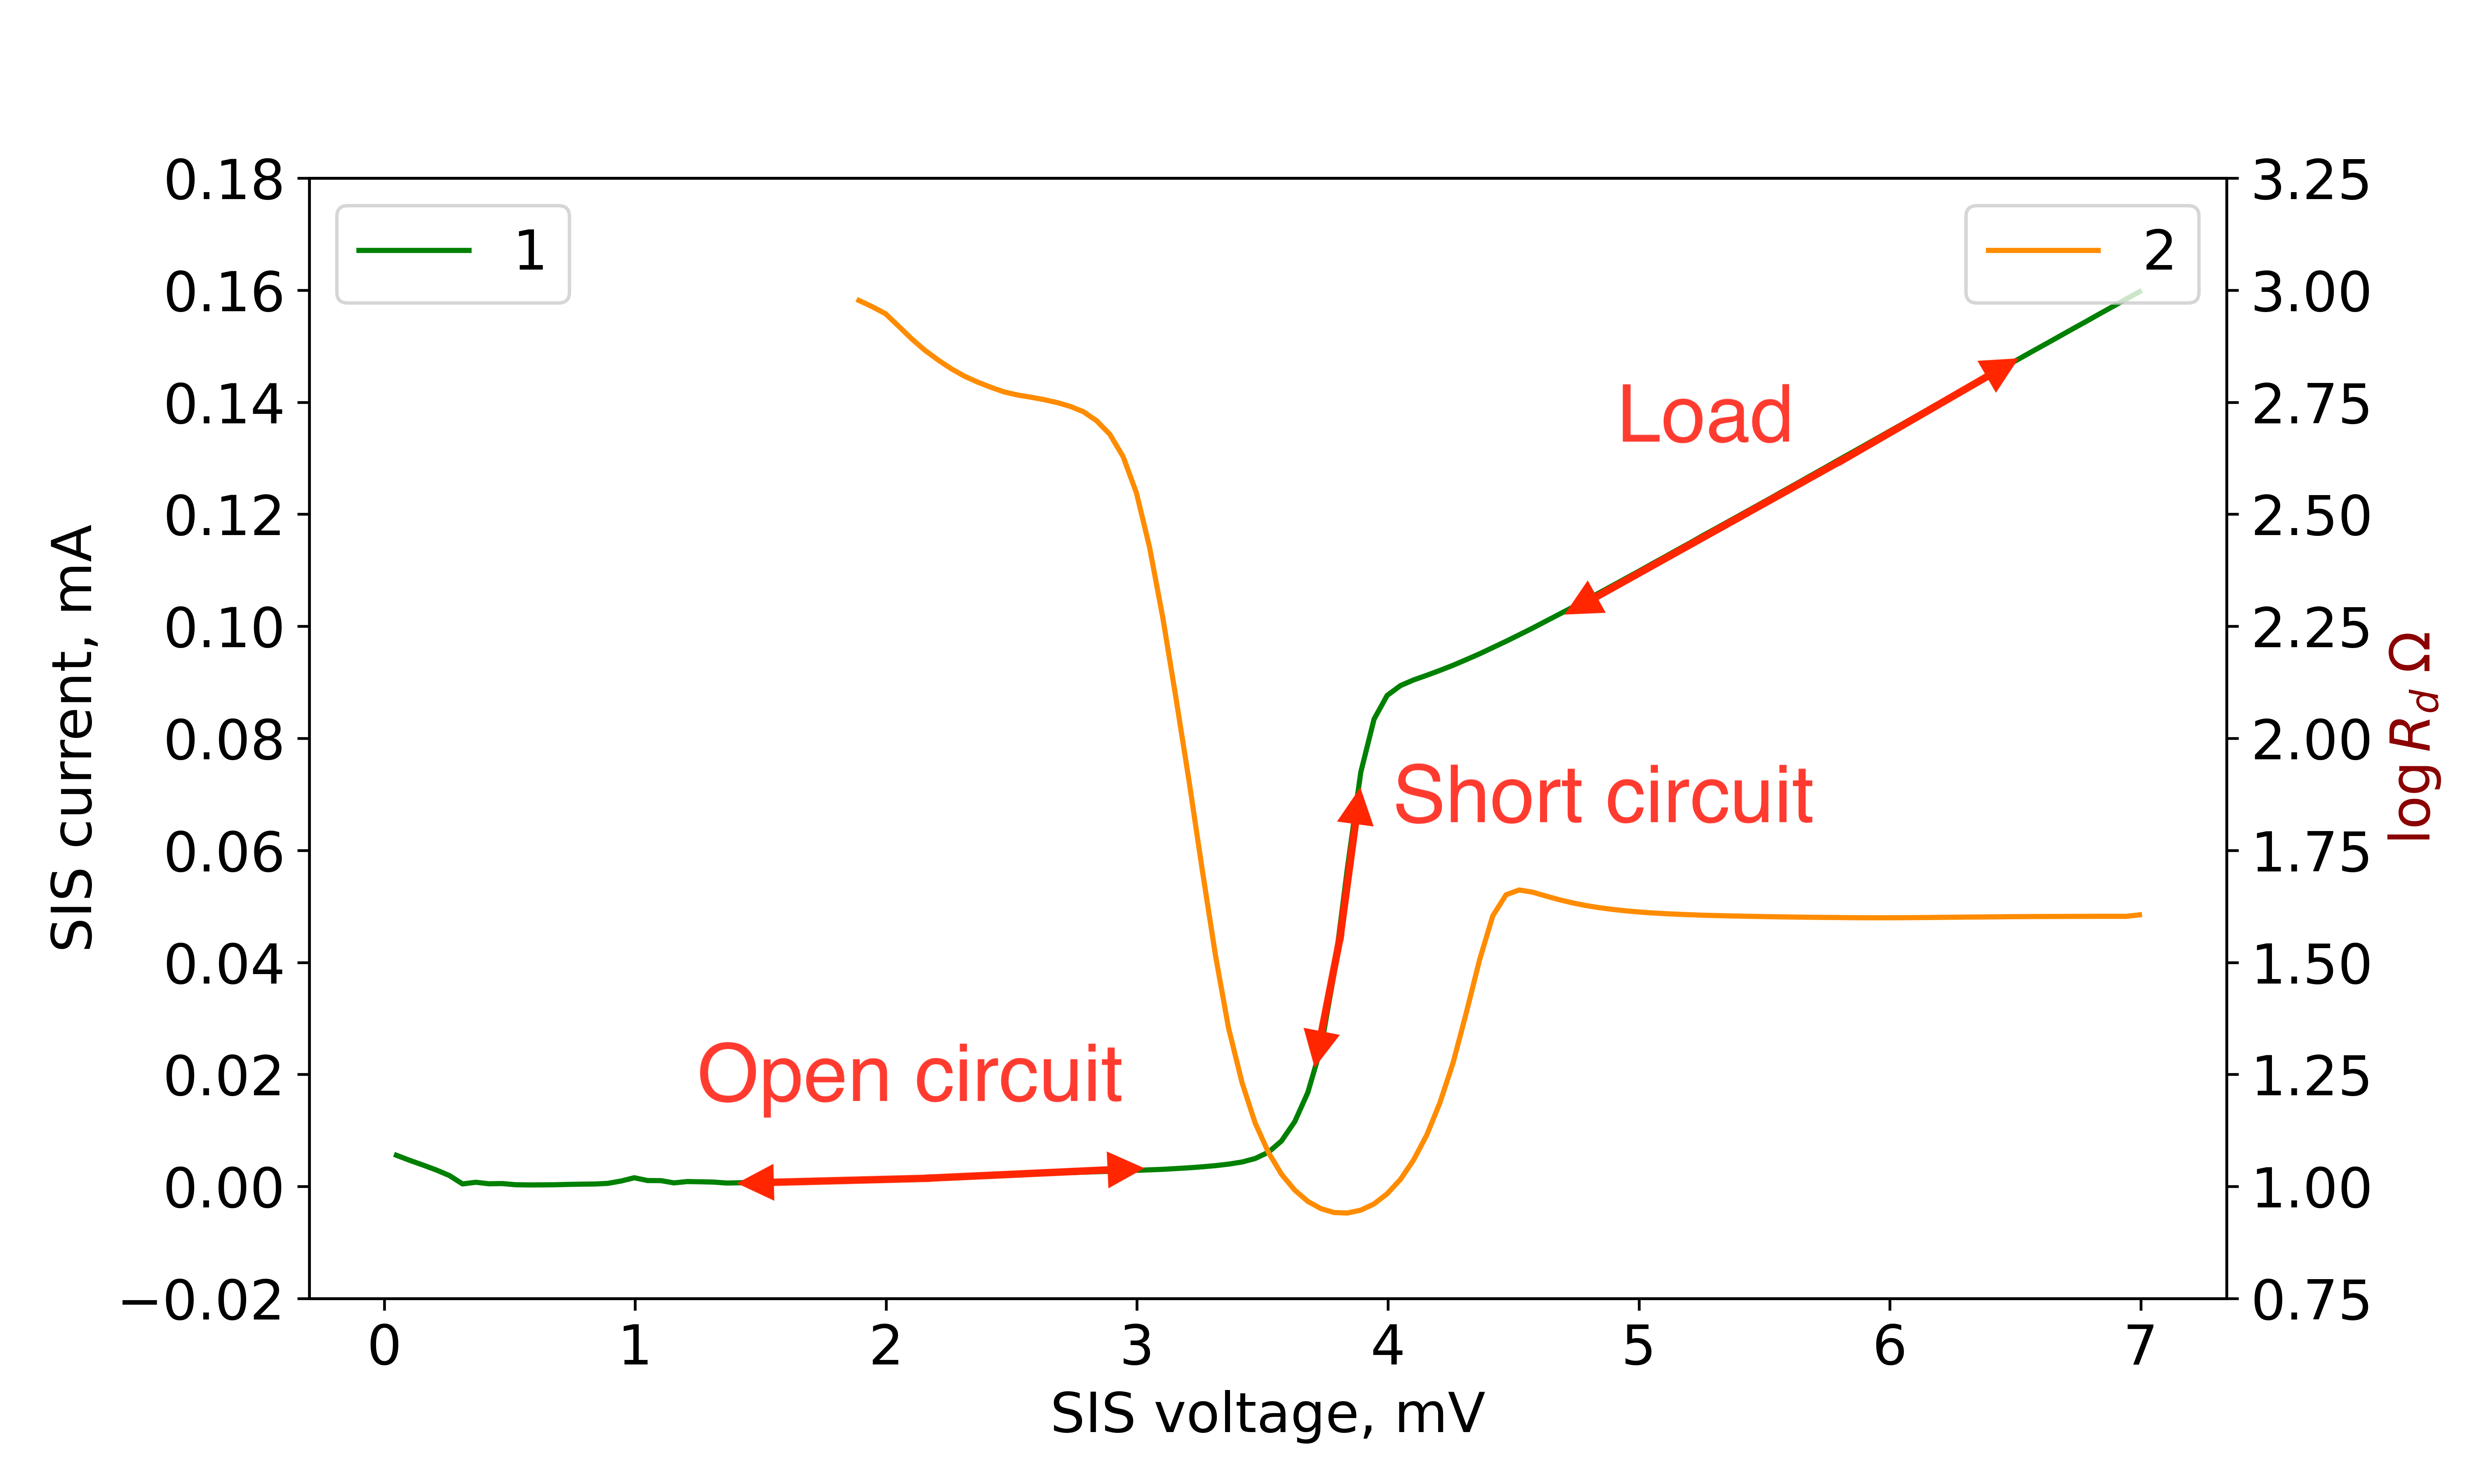
\includegraphics[scale=0.5]{cal.png}
        \caption{Автономная Вольт-амперная характеристика СИС-смесителя №1 зеленая линия; соответствующее дифференциальное сопротивление показано оранжевой линией №2.}
        \label{pic-cal}
    \end{center}
\end{figure}

\begin{figure}[H]
    \begin{center}
        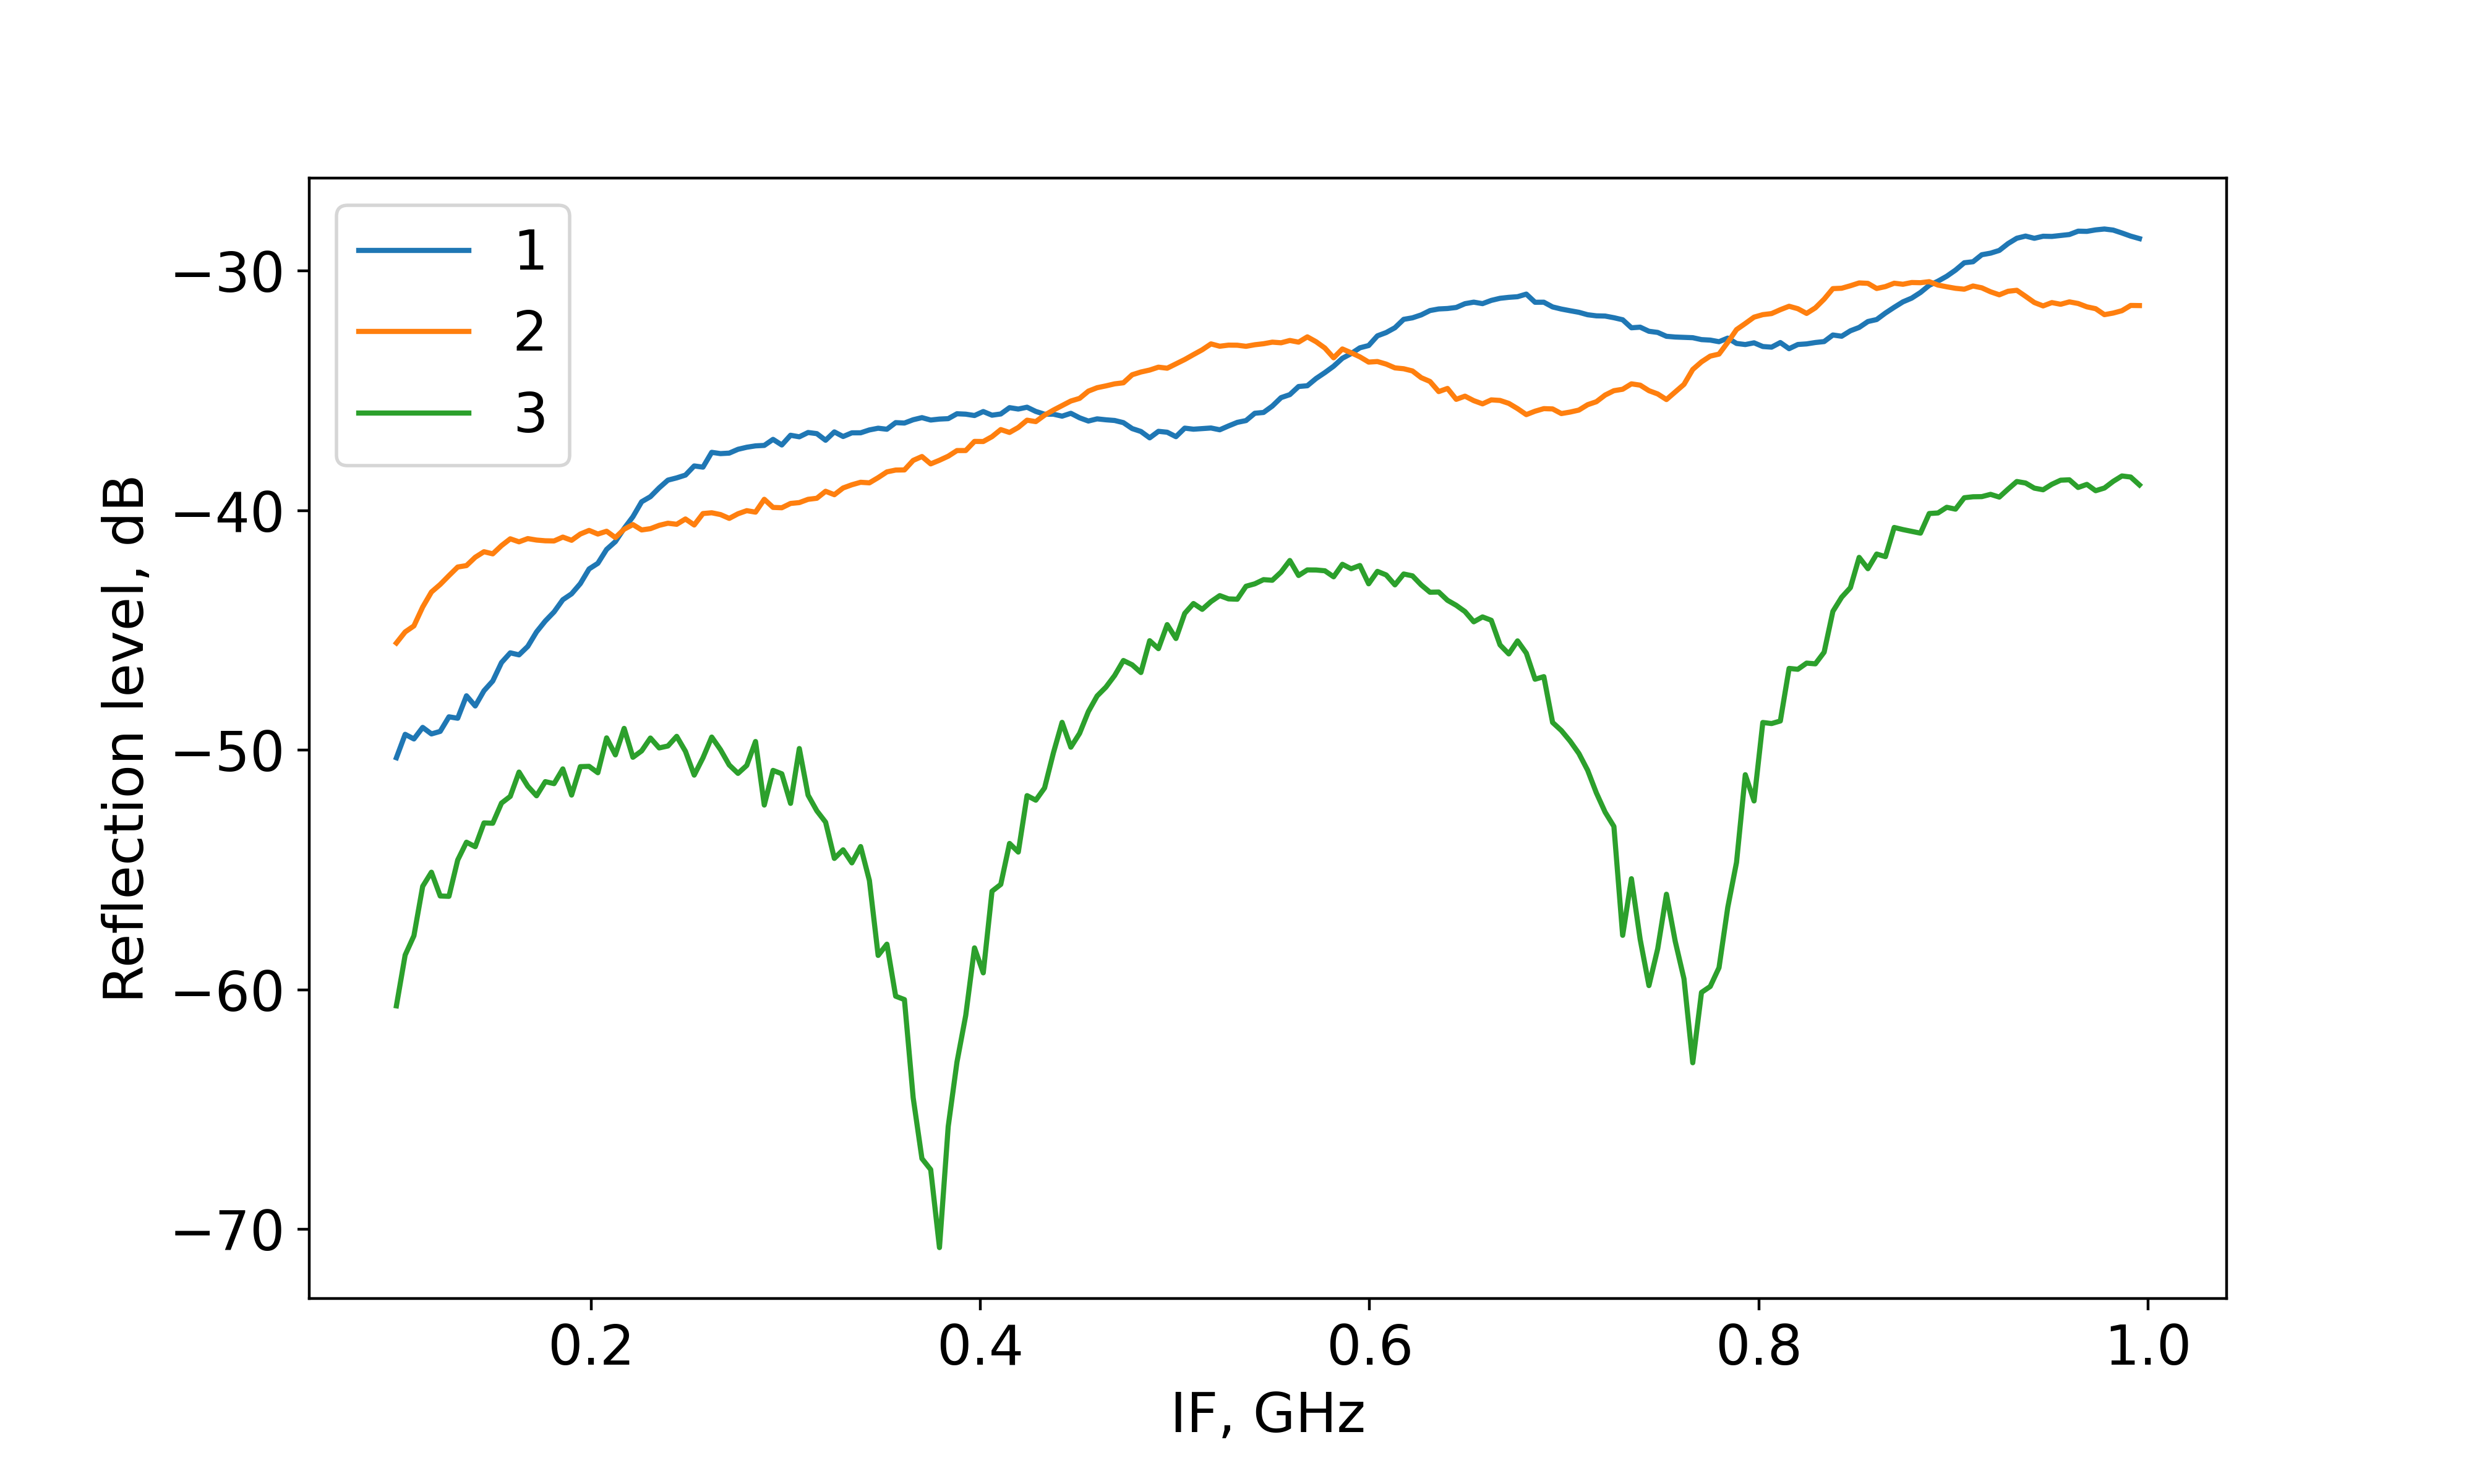
\includegraphics[scale=0.5]{cals.png}
        \caption{Пример калибровочных измерений: №1 — "открытая цепь"; №2 — "короткое замыкание"; №3 — "нагруженная линия"}
        \label{pic-cals}
    \end{center}
\end{figure}

\begin{figure}[H]
    \begin{center}
        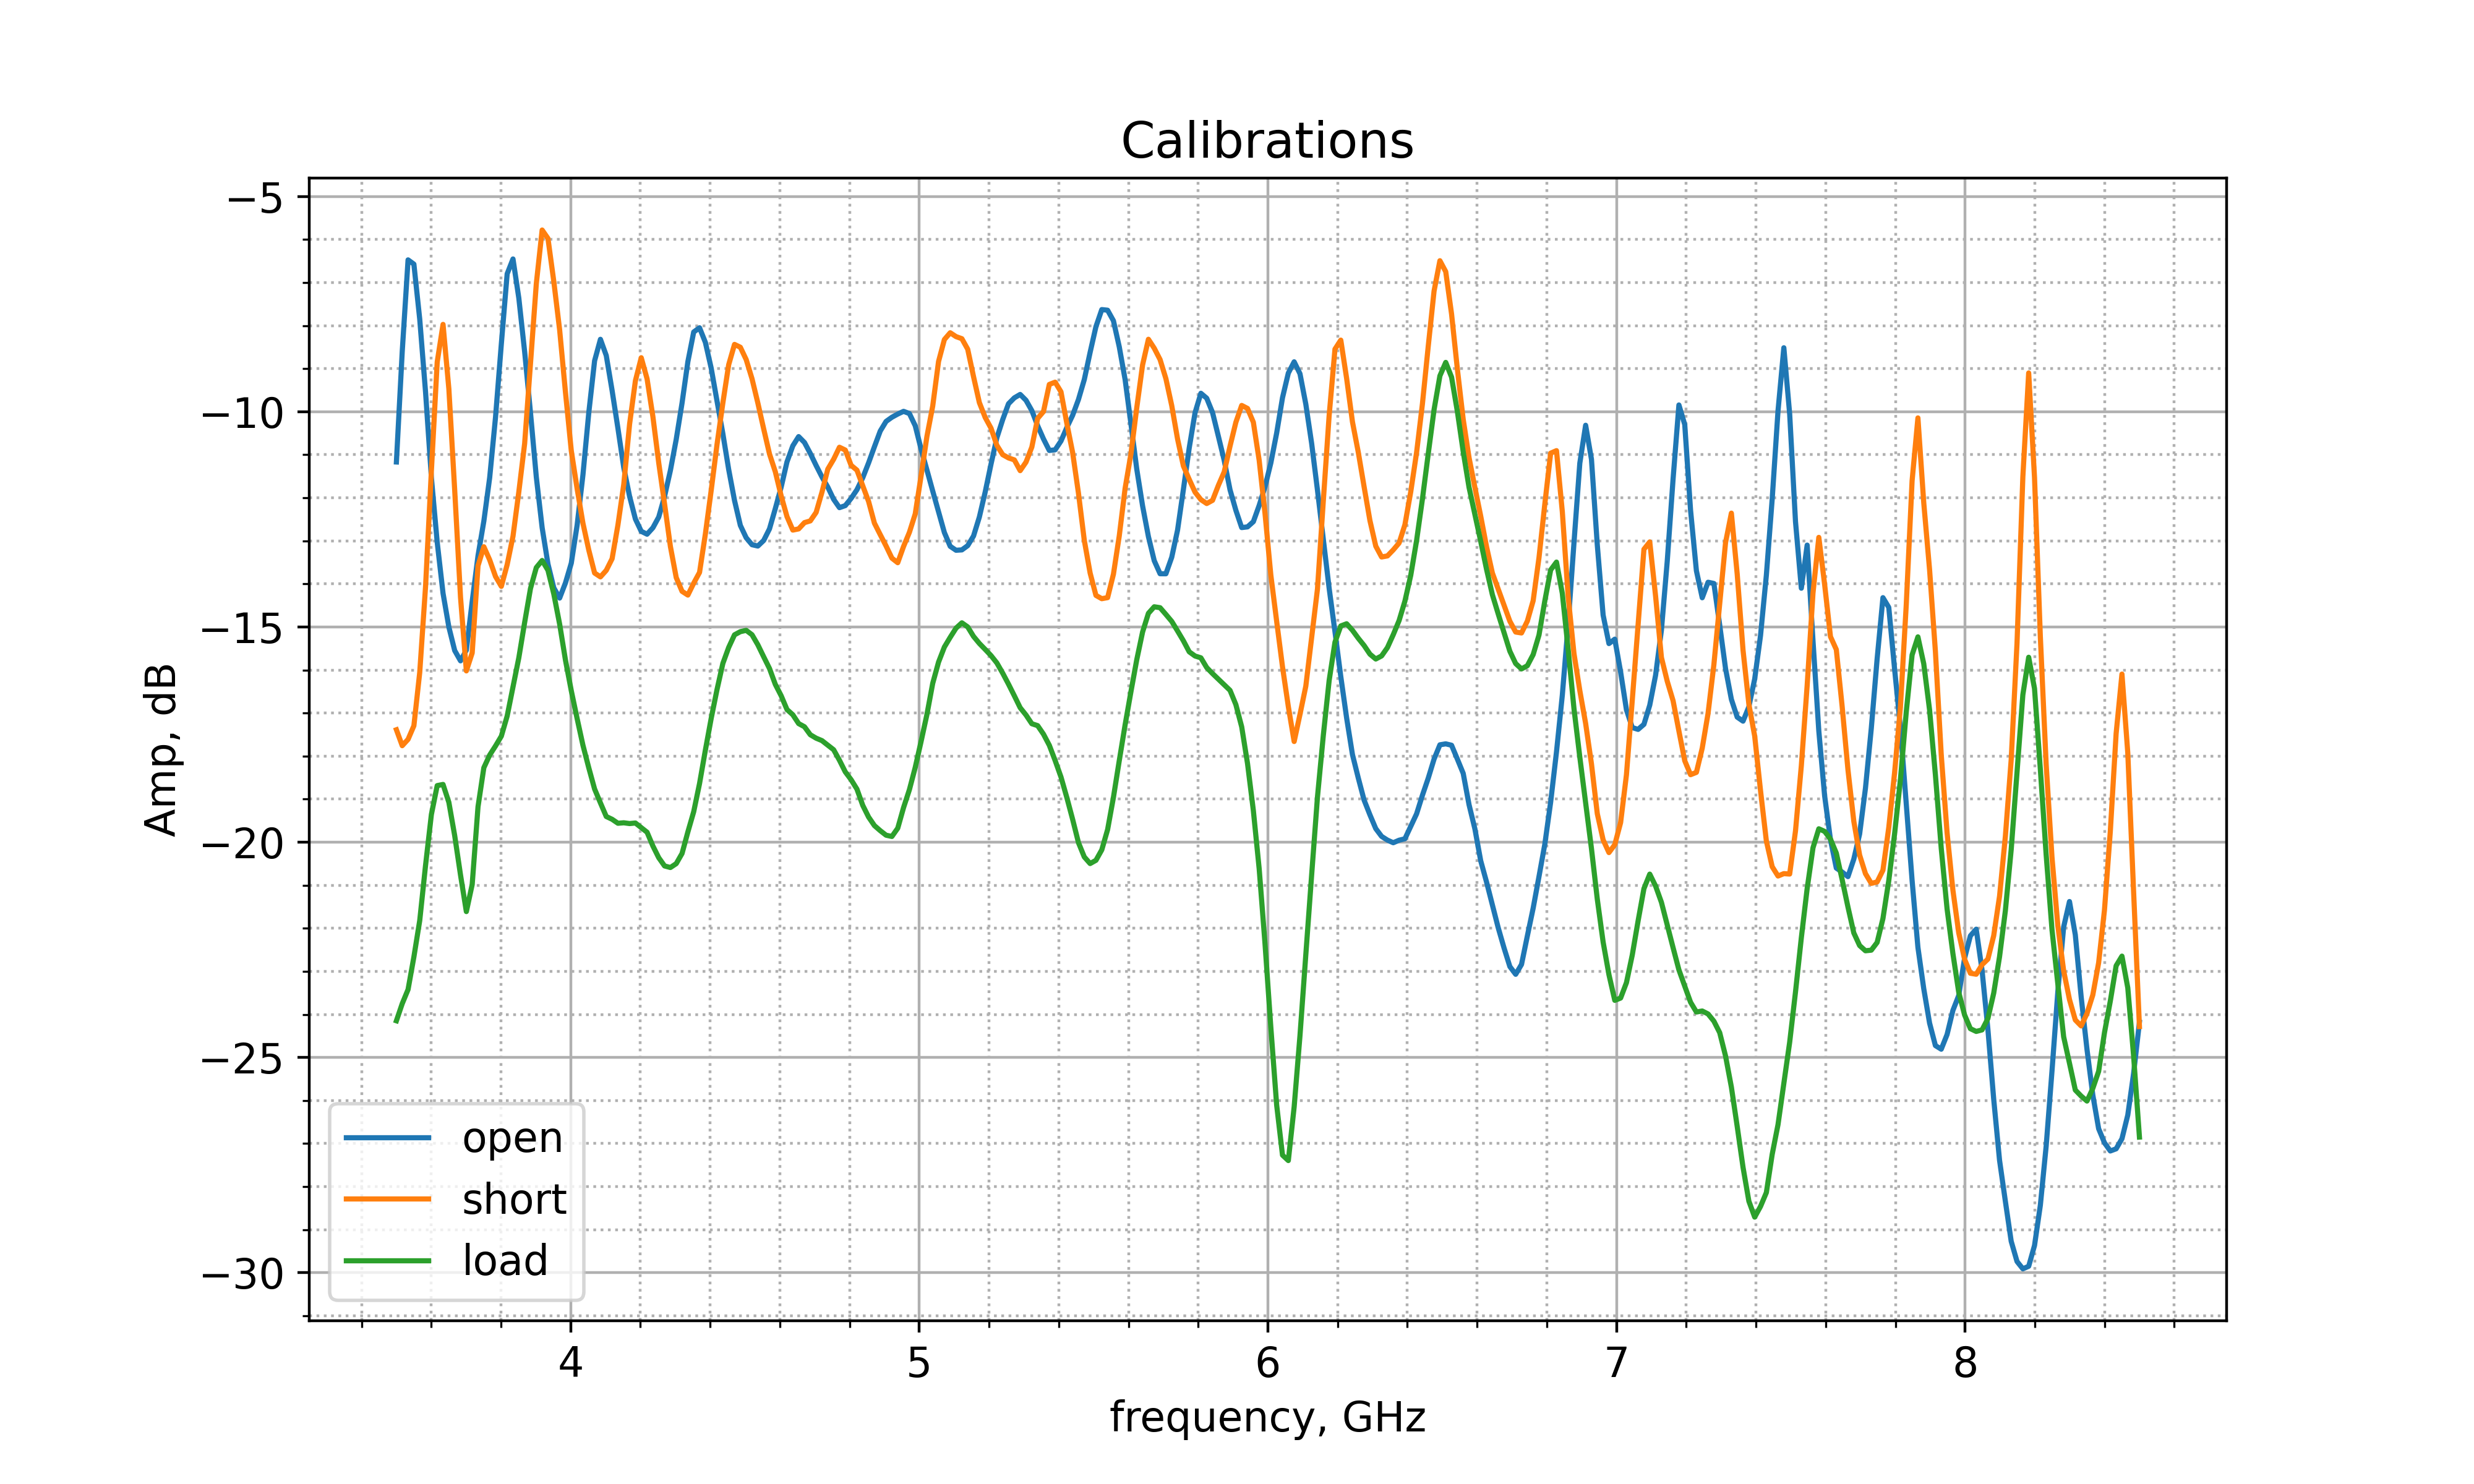
\includegraphics[scale=0.5]{cals2.png}
        \caption{Пример калибровочных измерений для волноводного СИС-смесителя диапазона 211-275 ГГц: open — "открытая цепь"; short — "короткое замыкание"; load — "нагруженная линия"}
        \label{pic-cals2}
    \end{center}
\end{figure}

Обратим внимание, что кривые №1,2 и open, short на рис.\ref{pic-cals} и \ref{pic-cals2} соответственно находятся в противофазе, это обьясняется тем, что при отражении электро-магнитной волны от среды с очень маленьким сопротивлением (короткое замыкание) происходит скачек фазы на $\pi$, в отличии от случая отражения от очень большого сопротивления (открытая цепь).

Этих трех калибровок достаточно, чтобы составить 3 уравнения (\ref{eq:sys}) используя (\ref{gamma}) и тем самым определить коэффициенты D, R и M. Это позволяет учесть все отражения и 
утечки в цепи и корректно измерить отражение от СИС-смесителя в рабочем режиме. Стоит отметить, что в приведенной калибровке внутренняя емкость СИС-смесителя выступает 
как часть внешней цепи и ее влияние также нивелируется калибровкой.

\subsection{Теоретический рассчет отражения}

Величина отражений от СИС-смесителя по тракту ПЧ, характеризуемая параметром $S11_{IF}$  \cite{Kooi}, может быть определена, если известен выходной импеданс ПЧ СИС-смесителя $Z_{IF}$  и импеданс подводящей линии тракта ПЧ $Z_L$
\begin{equation}
    S11_{IF} = \frac{Z_{IF} - Z_L}{Z_{IF} + Z_L}
    \label{s11}
\end{equation}
Для расчета  мы используем 3х частотное приближение к теории квантового смешения Tucker \cite{Tucker}. Рассмотрены сигналы на частотах 
$f_m = m \cdot f_{LO} + f_0$, 
где $m = 0, \pm 1$; $f_{\pm}$  - верхняя и нижняя полосы; $f_{LO}$ - частота опорного генератора; $f_0$ - промежуточная частота. Полагаем, что более высокие гармоники шунтируются емкостью СИС-смесителя, составляющей в нашем случае порядка 100 фФ.
Принимая во внимание взаимодействие портов смесителя, компоненты напряжений и токов слабых сигналов линейно связаны матрицей проводимости $i_m = \sum_{m'} Y_{mm'}' \upsilon_{m'} $ :
\begin{equation}
    Y_{mm'}' (V_{gap}, R_N, f_{LO}, \alpha, V_0) = 
    \begin{bmatrix}
        Y_{11} + Y_{S} & Y_{10} & Y_{1-1}  \\
        Y_{01} & Y_{00} + Y_L & Y_{0-1}   \\
        Y_{-11} & Y_{-10} & Y_{-1-1}+Y_I  \\
    \end{bmatrix}
    \label{Y_mm}
\end{equation}
где $V_{gap}$ - напряжение смещения туннельного скачка тока, $R_N$ - нормальное дифференциальное сопротивление ВАХ, $\alpha = e V_{LO} / h f_{LO}$ - безразмерный параметр накачки, 
пропорциональный напряжению опорного генератора $V_{LO}$ , $V_0$ - напряжение смещения СИС-смесителя.
\par

У каждого порта есть своя канальная проводимость: $Y_1 = Y_S$ - нагрузка порта с принимаемым сигналом, $Y_0 = Y_L$ - нагрузка порта ПЧ, $Y_{-1}=Y_I$ - нагрузка порта нижней полосы.
\begin{figure}[H]
    \begin{center}
        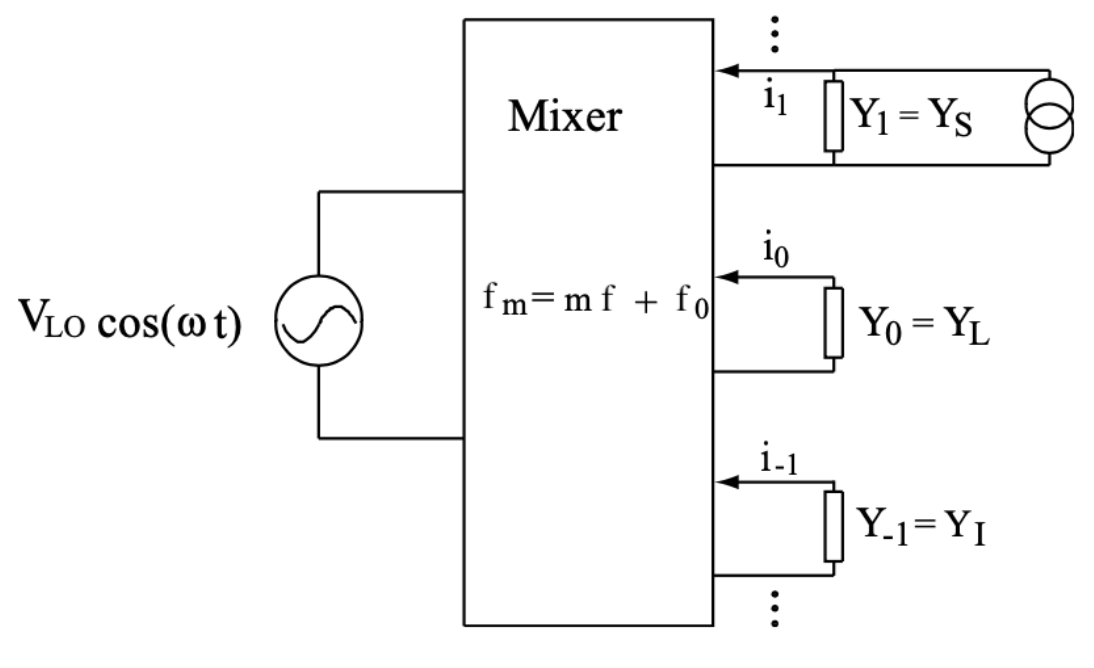
\includegraphics[scale=0.5]{mixer_scheme.png}
        \caption{Эквивалентная схема гетеродинного смесителя, с приложенным сигналом опорного генератора частоты , принимаемым сигналом частоты  и сигналом ПЧ}
        \label{mixer_scheme}
    \end{center}
\end{figure}

Для  идеального двухполосного  смесителя  импедансы верхней и нижней полос равны $Y_1 = Y_{-1}$. В нашем случае $Y_{\pm 1}$ - результат преобразования проводимости  опорного генератора несколькими микрополосковыми линиями.
\par 

Воспользовавшись результатом \cite{Tucker}, получим $Y_{mm'} = G_{mm'} + i B_{mm'}$ , где

\begin{equation}
    \begin{split}
    G_{mm\prime} = \frac{e}{2 \hbar \omega_{m\prime}} 
    \cdot \sum_{n,n\prime=-\infty}^{\infty} J_n(\alpha) J_{n\prime}(\alpha) \delta_{m-m\prime, n\prime-n} \\
    \left\{ \left[ I_{dc}(V_0+n\prime \hbar \omega /e + \hbar \omega_{m\prime}/e) - 
    I_{dc}(V_0 + n\prime \hbar \omega/e) \right] + \right. \\
    \left. \left[ I_{dc}(V_0 + n\hbar \omega/e) - 
    I_{dc}(V_0 + n \hbar \omega/e - \hbar \omega_{m\prime}/e) \right]  \right\}
    \end{split}
\end{equation}

\begin{equation}
    \begin{split}
        B_{mm\prime} = \frac{e}{2 \hbar \omega_{m\prime}} \cdot 
        \sum_{n,n\prime=-\infty}^{\infty} J_n(\alpha) J_{n\prime}(\alpha) \delta_{m-m\prime, n\prime-n} \\
        \left\{ \left[ I_{kk}(V_0+n\prime \hbar \omega /e + \hbar \omega_{m\prime}/e) - 
        I_{kk}(V_0 + n\prime \hbar \omega/e) \right] - \right. \\
        \left. \left[ I_{kk}(V_0 + n\hbar \omega/e) - 
        I_{kk}(V_0 + n \hbar \omega/e - \hbar \omega_{m\prime}/e) \right]  \right\}
    \end{split}
\end{equation}

Где $I_{dc}(V_0)$ - зависимость туннельного тока СИС-смесителя от его напряжения; $I_{kk}(V_0)$ - зависимость соотношения Крамерса-Кронига тока $I_{dc}$ от напряжения СИС-смесителя; 
$J_n(\alpha)$ - функция Бесселя порядка  от параметра накачки $\alpha$ .
Тогда, в нашем случае импеданс по ПЧ:
\begin{equation}
    Z_{IF} = \left \| Y_{mm'} + Y_{m} \delta_{mm'} \right \|^{-1}_{00}
    \label{eq:z}
\end{equation}

На рис.\ref{pic-IV} продемонстрирована измеренная ВАХ СИС-перехода, которая является зависимостью $I_{dc}(V_0)$ и определяет $I_{kk}$. 
Автономная кривая показана зеленой линией, при этом, оранжевой кривой показана ВАХ для случая, когда приложен внешний сигнал генератора частотой 600 ГГц. 

\begin{figure}[H]
    \begin{center}
        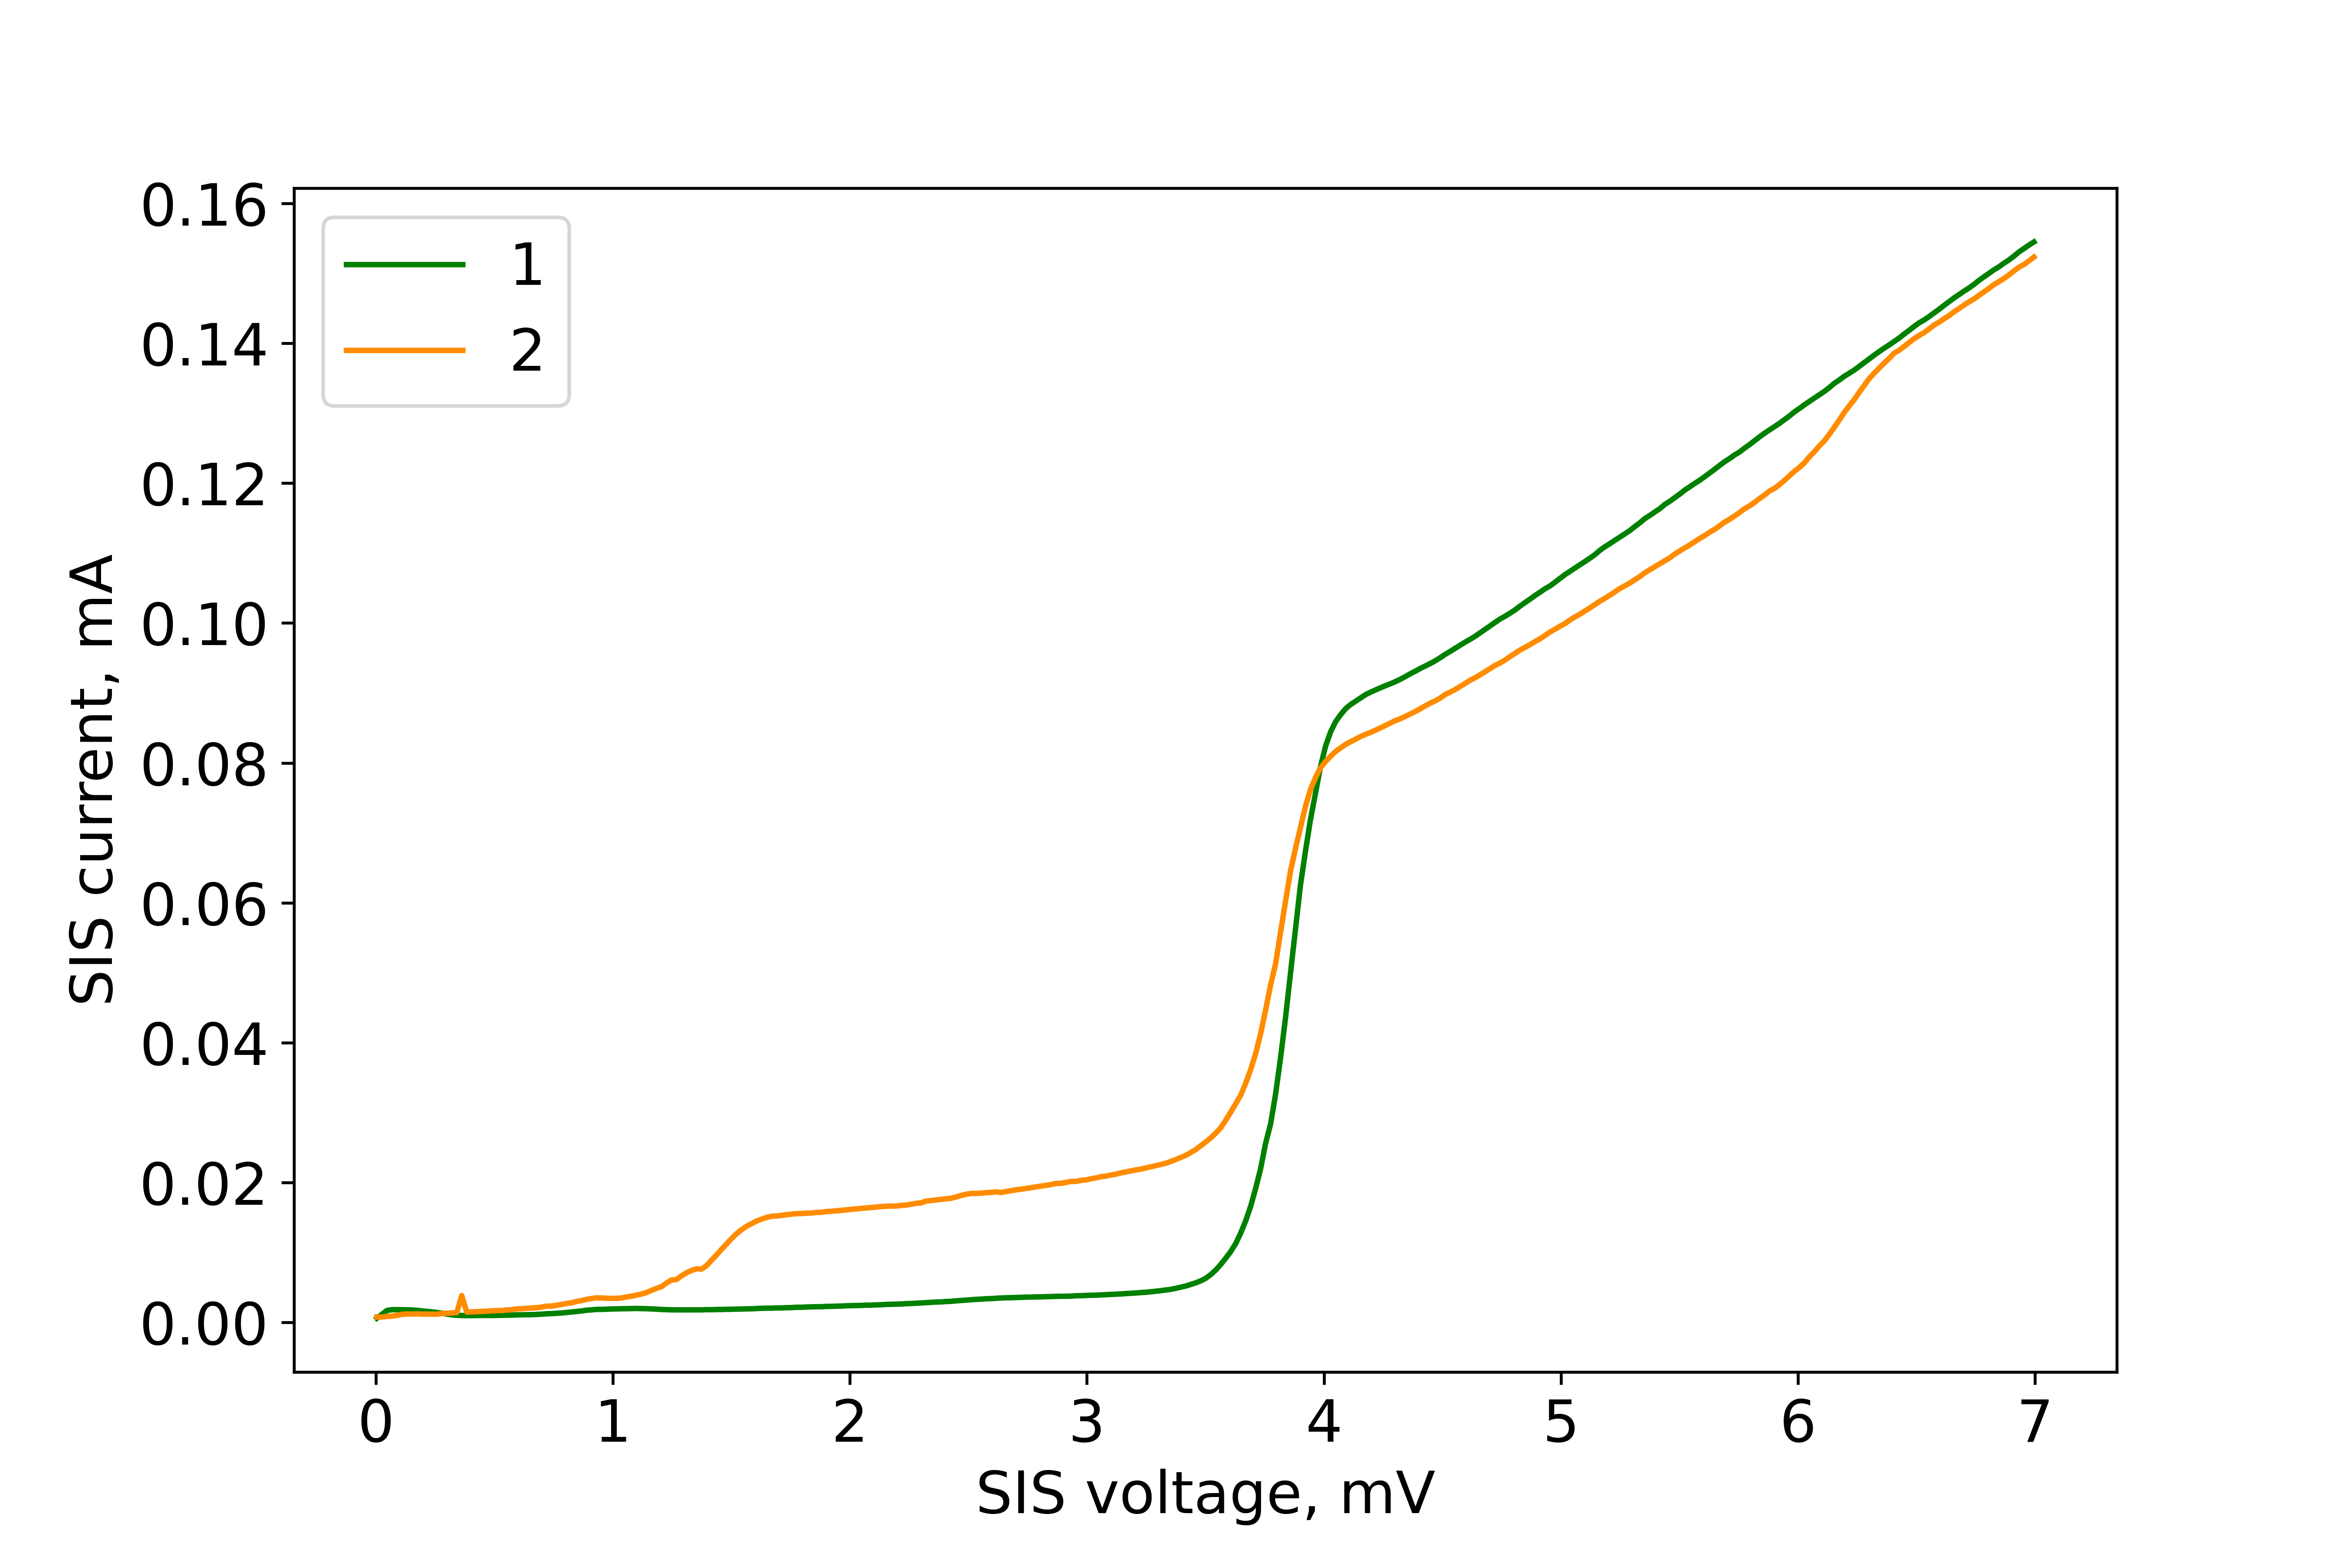
\includegraphics[scale=0.5]{IV.png}
        \caption{Экспериментальная ВАХ автономная (№1 зеленая кривая) и с приложенным сигналом опорного генератора (№2 оранжевая кривая).}
        \label{pic-IV}
    \end{center}
\end{figure}

На рис. \ref{pic-reim} приведен результат теоретического расчета импеданса с использованием ВАХ (рис.\ref{pic-IV}) в диапазоне ПЧ 0.1-12 ГГц при различных напряжениях на СИС-переходе: 2.8, 3, 3.2 мВ, 
причем импеданс подводящей линии полагается $\sim 50$ Ом. Можно заключить, что действительная часть изменяется незначительно с промежуточной частотой, в отличие от мнимой части. 
Также видно, что импеданс сильно зависит от напряжения на СИС-переходе.

\begin{figure}[H]
    \begin{center}
        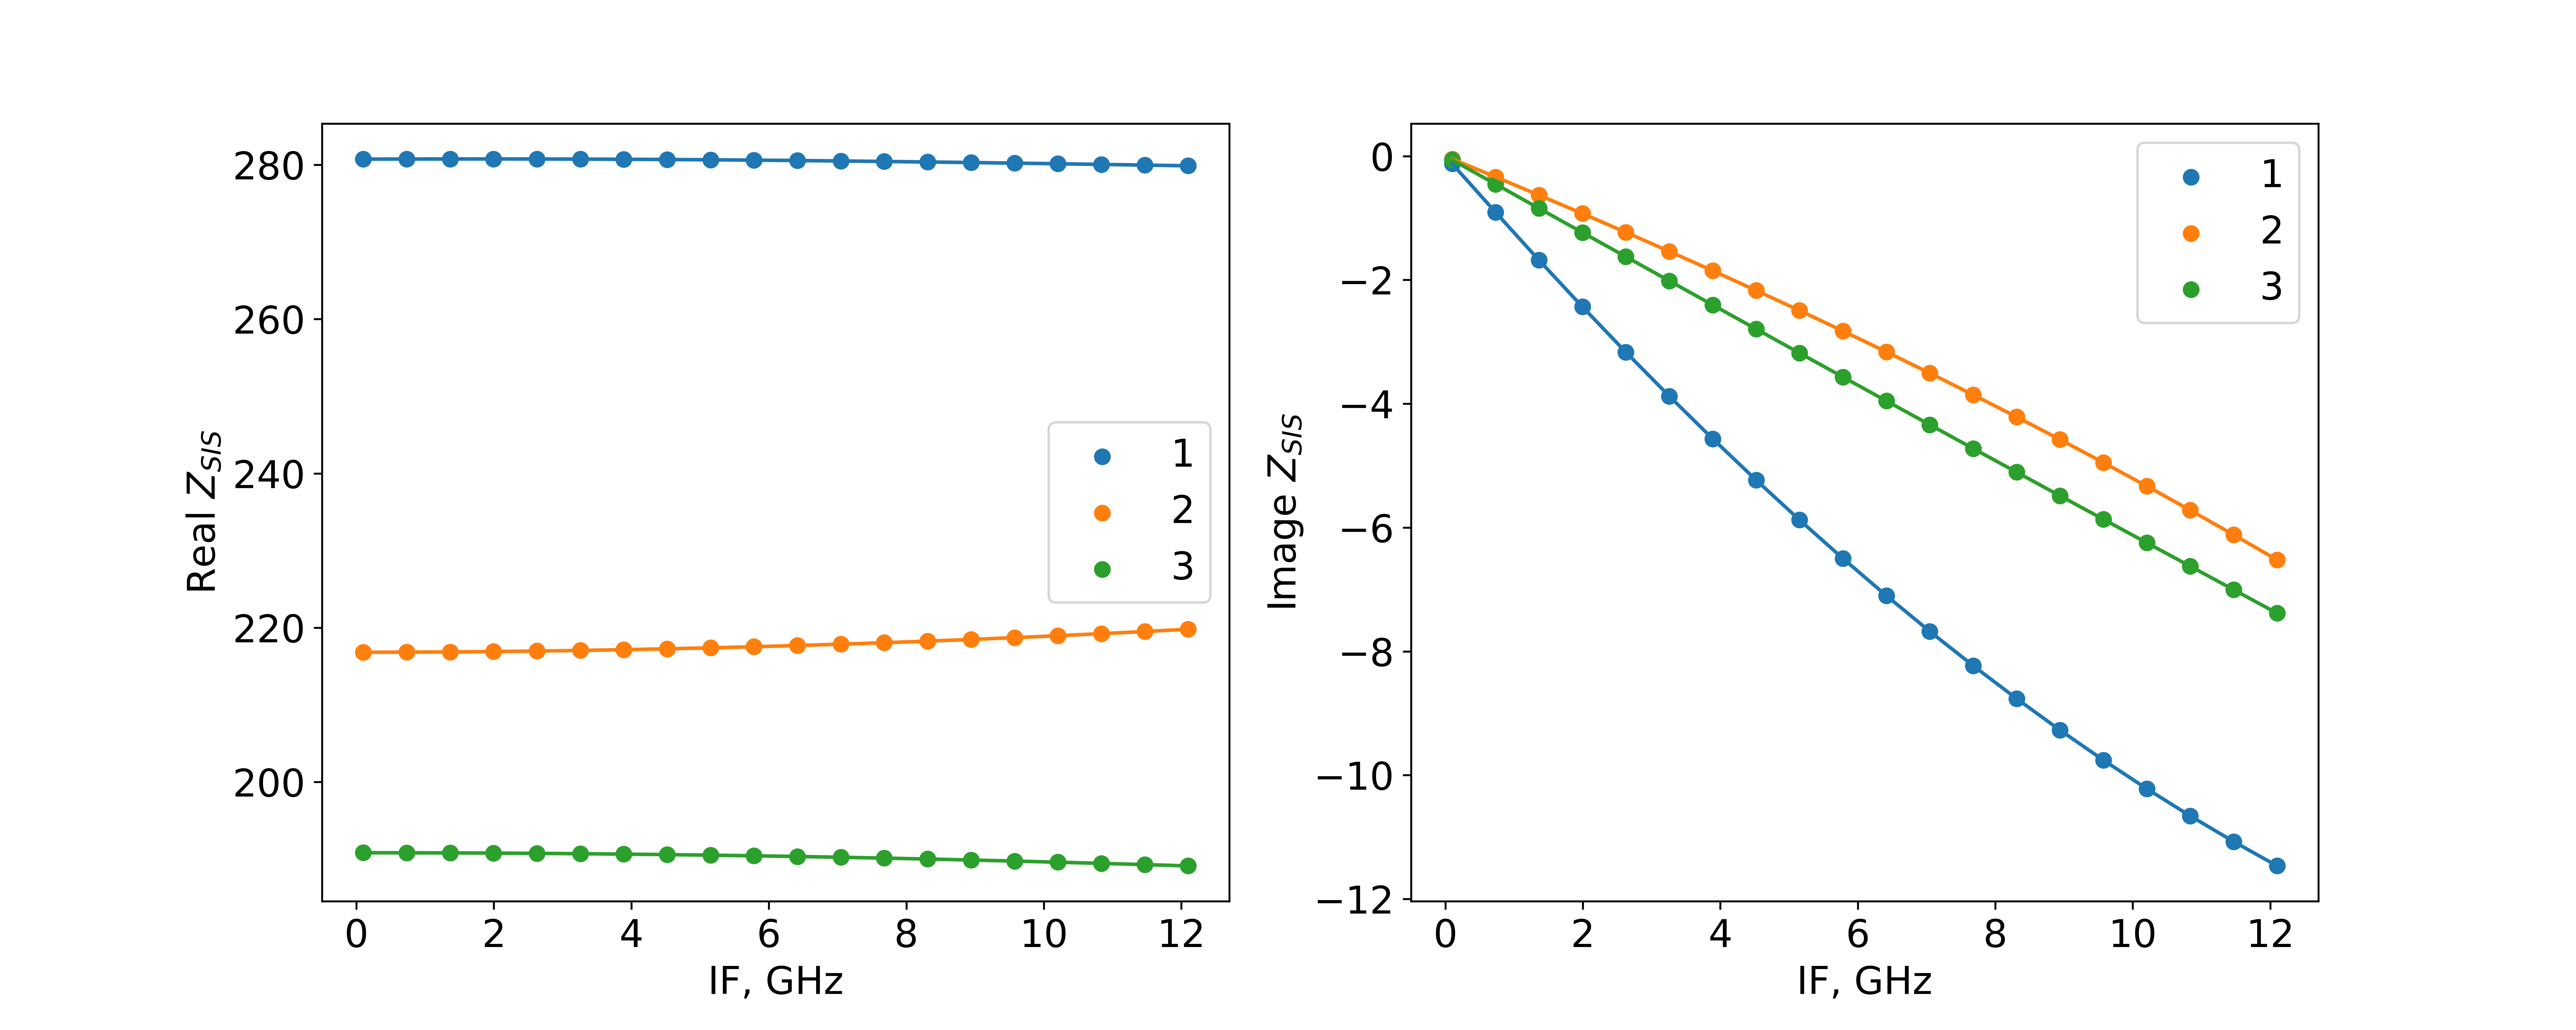
\includegraphics[scale=0.4]{reim.png}
        \caption{Действительная (слева) и мнимая (справа) части расчетного импеданса СИС-смесителя от ПЧ при разных напряжениях на СИС-смесителе; №1 – 2.8 мВ, №2 – 3 мВ, №3 – 3.2 мВ.}
        \label{pic-reim}
    \end{center}
\end{figure}


\subsection{Результаты измерений}

\subsubsection{Частотная характеристика}

 ВАХ интегрального СИС-смесителя, при приложении сигнала опорного генератора частотой  ГГц в «рабочем» режиме, показана на рис.\ref{pic-IV}  оранжевой кривой. Диапазон «рабочего» напряжения смещения лежит приблизительно в интервале 1.6–3.4 мВ. Эта область напряжений соответствует так называемой квазичастичной ступени, вызванной приложением к СИС-переходу сигнала гетеродина. На рис.\ref{pic-refl_if} приведены экспериментальные (непрерывные кривые) и теоретические (пунктирные кривые) частотные зависимости уровня отражения при различных напряжениях на СИС-смесителе. Из приведенных результатов видно, что в диапазоне 4–8 ГГц уровень отражения почти не меняется с частотой, что хорошо согласуется и с теоретическими предсказаниями. 
 
\begin{figure}[H]
    \centering
    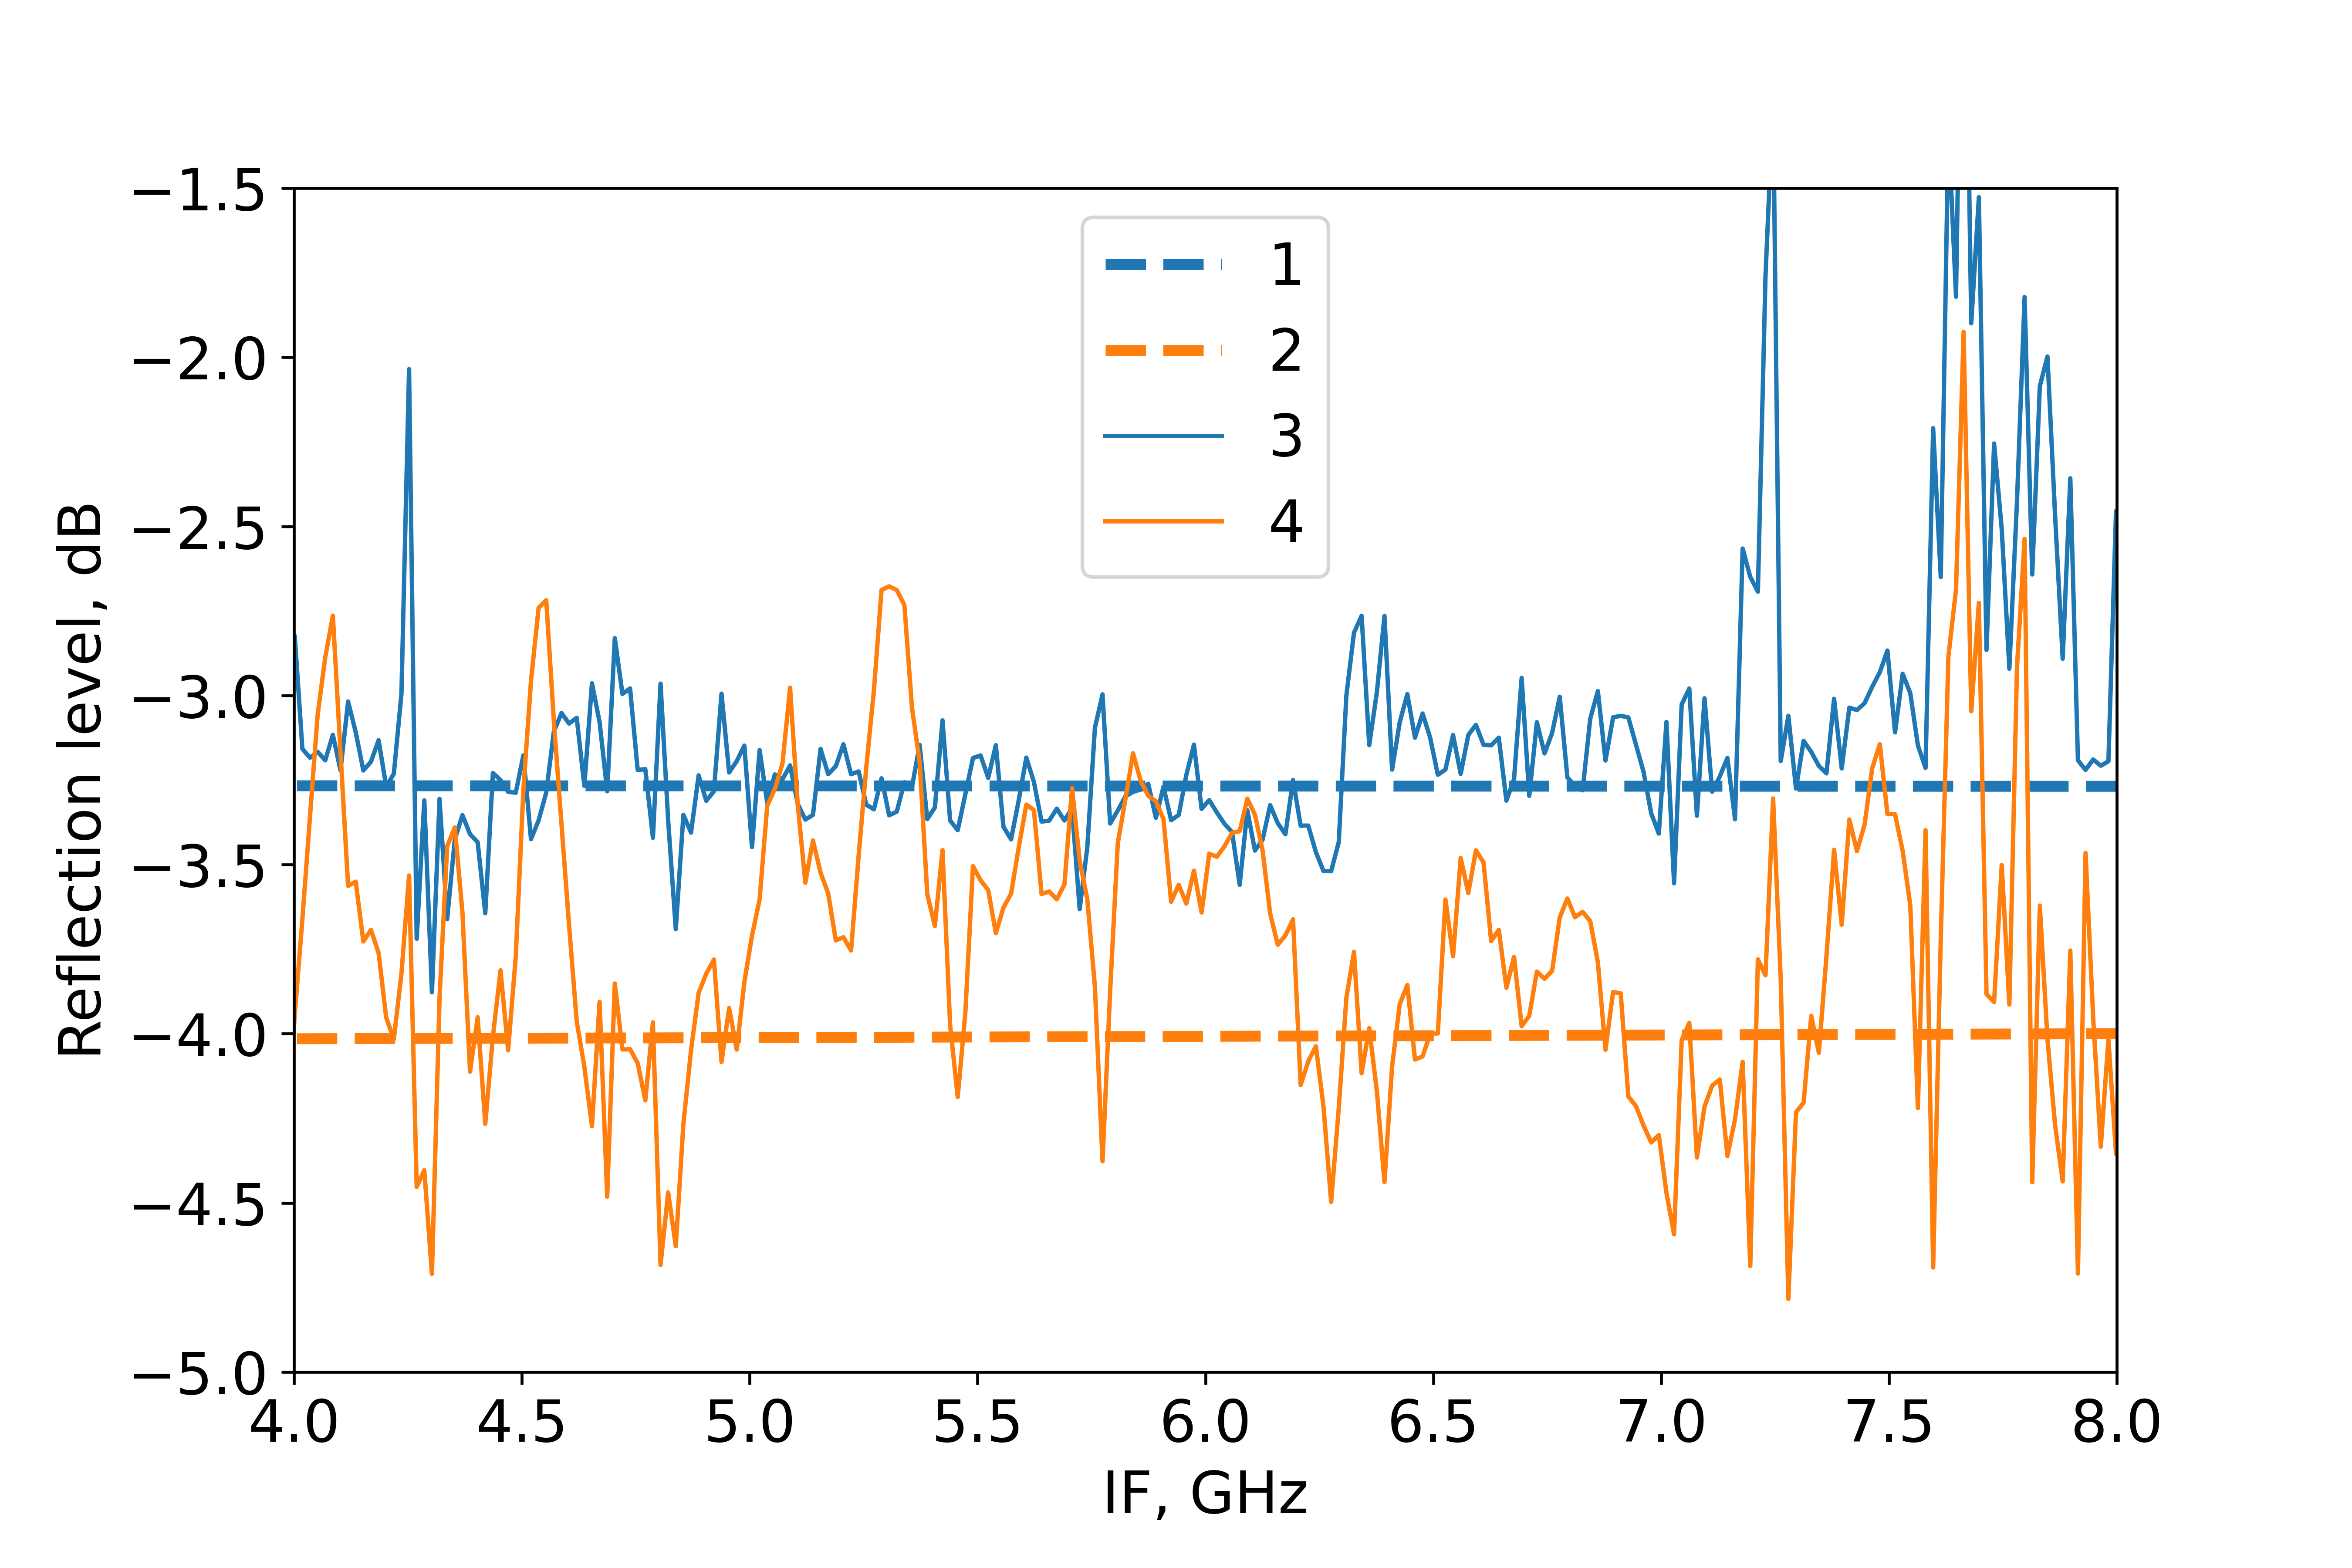
\includegraphics[scale=0.5]{refl_if.png}
    \caption{Рассчитанный теоретически (№ 1,2 пунктирные линии) и определенный экспериментально (№ 3,4 сплошные кривые) уровень отражения от СИС-перехода в «рабочем режиме»; Напряжения СИС-смесителя № 1,3 –  2 мВ, № 2,4 – 2.6 мВ}
    \label{pic-refl_if}
\end{figure}

Аналогично приведен пример измеренного отражения по тракту ПЧ от волноводного СИС-смесителя, при приложенном сигнале опорного генератора 230 ГГц на рис. \ref{fig:refl_new}. Можно заключить, что уровень отражения не имеет явной зависимости от ПЧ, однако в данном случае результаты искажены некорректной работой криогенного усилителя.

\begin{figure}[H]
    \centering
    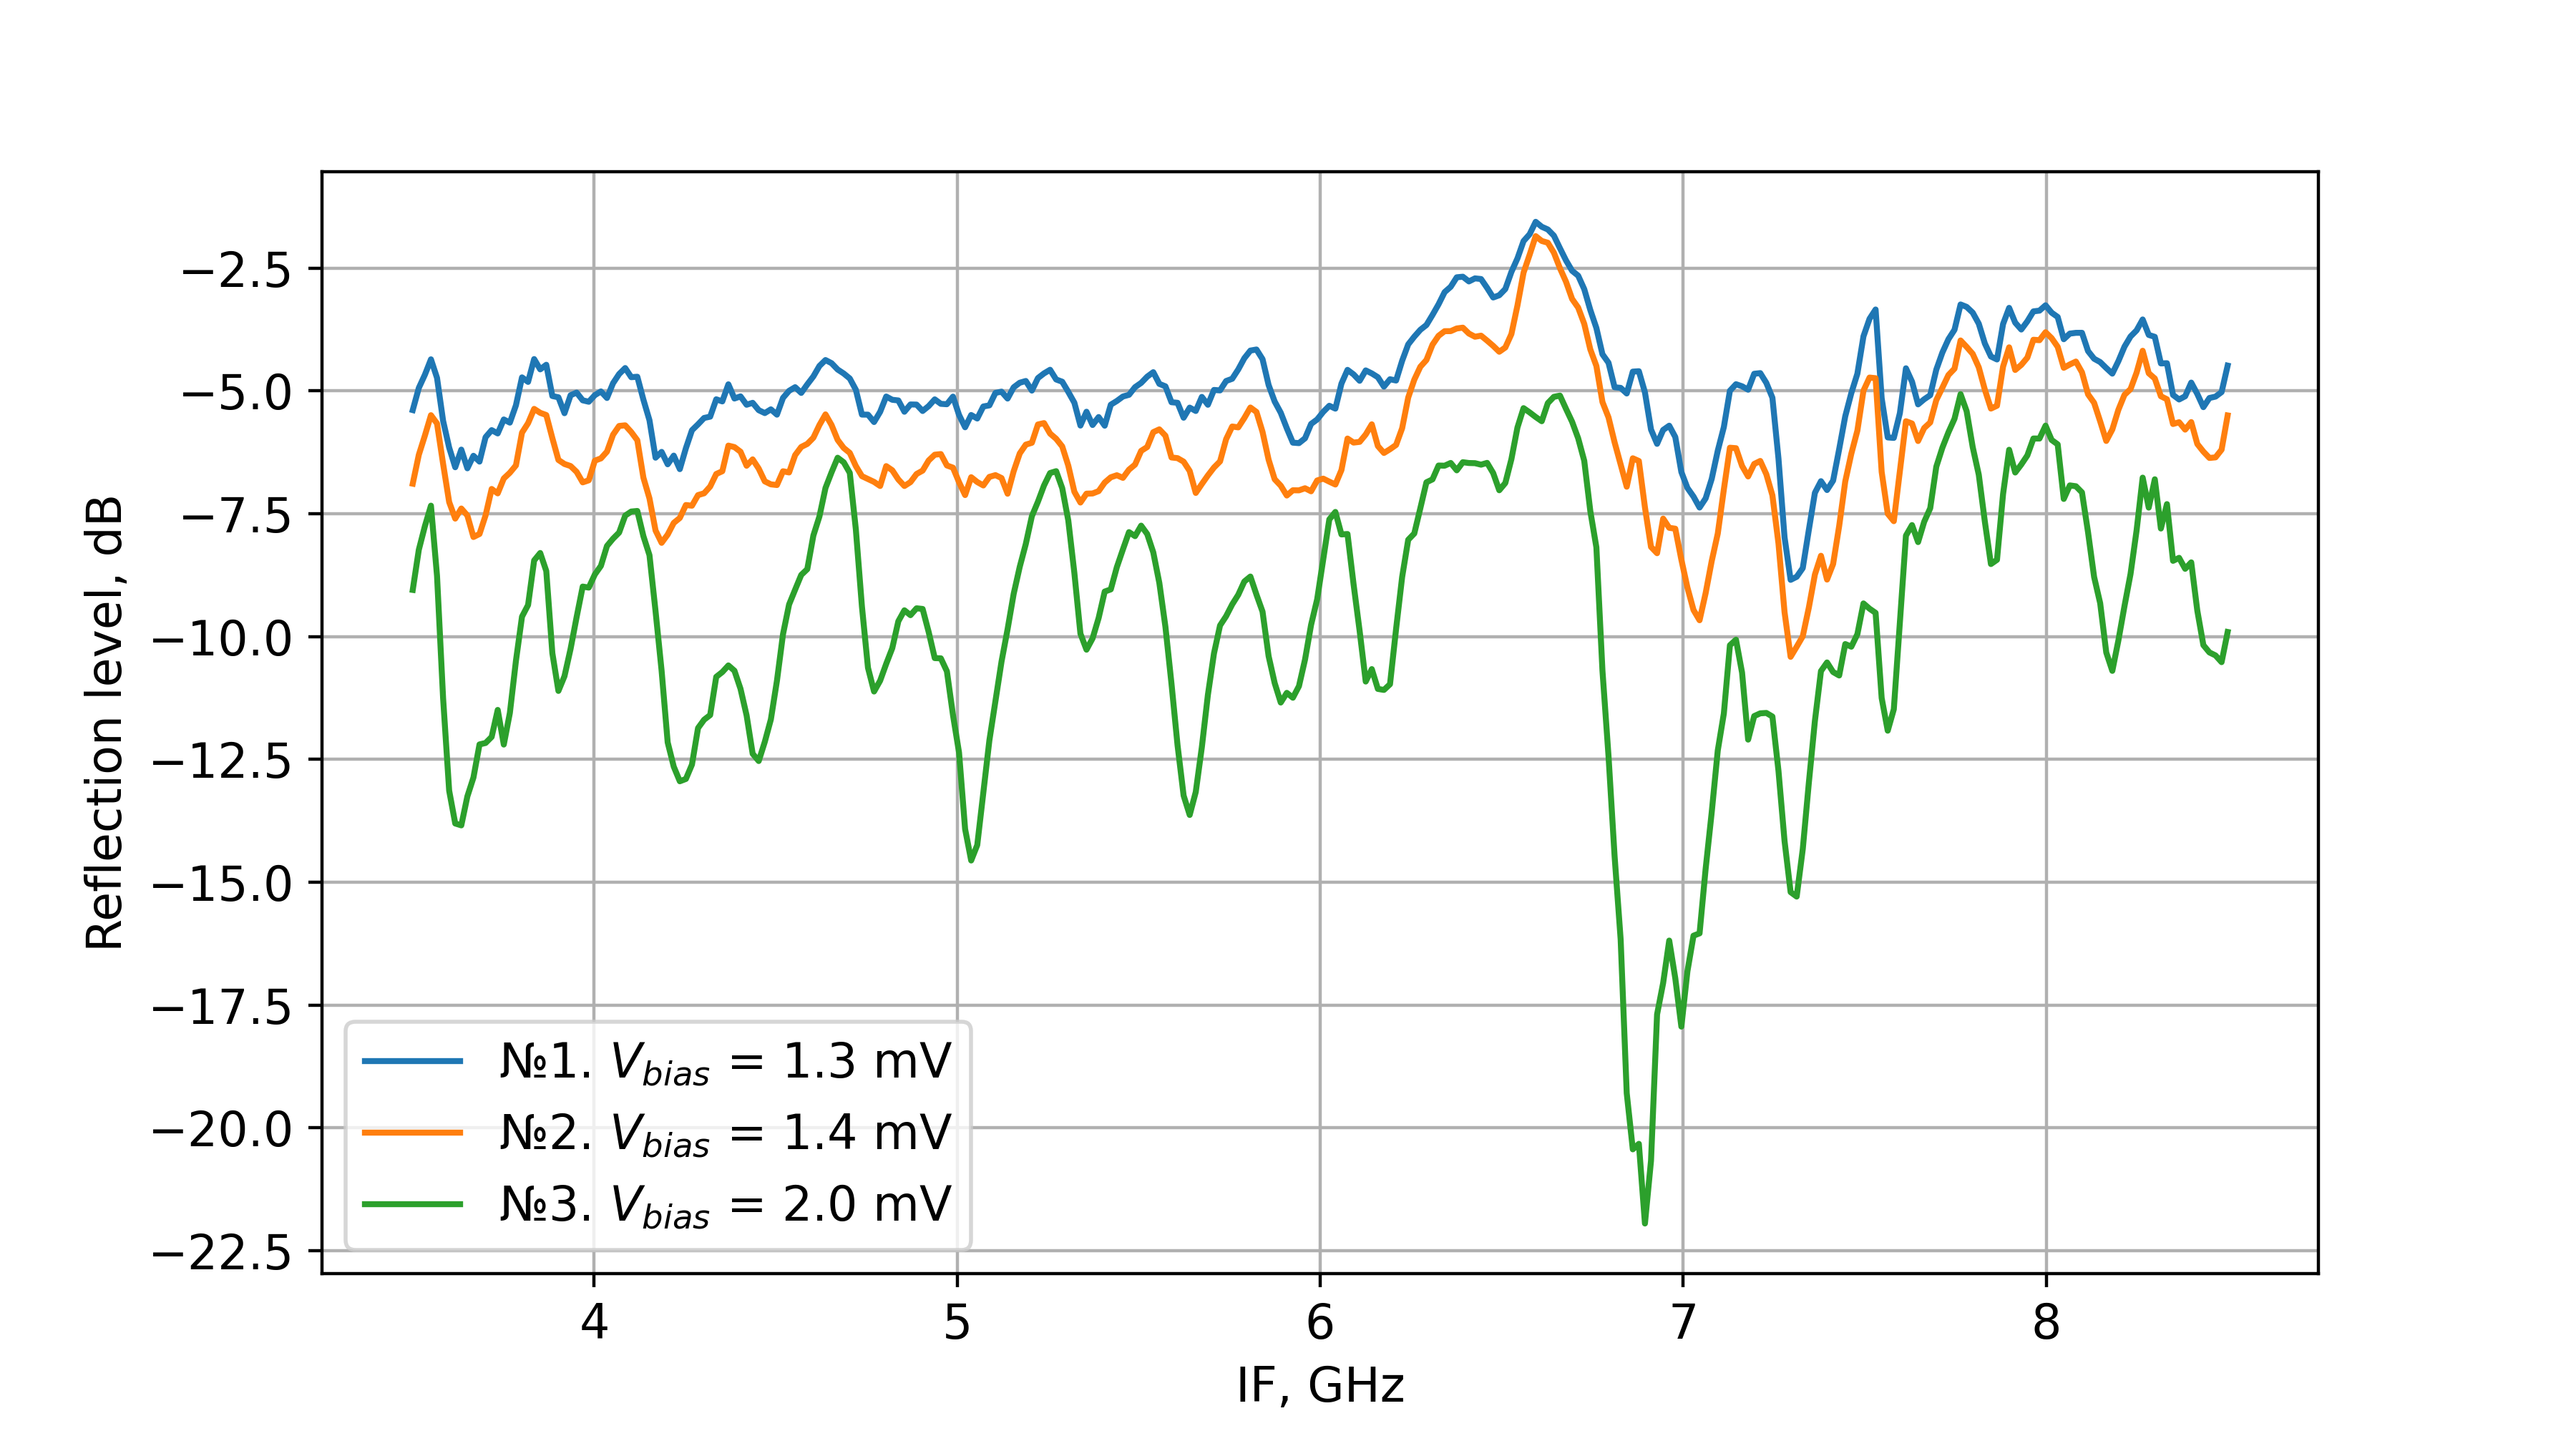
\includegraphics[scale=0.5]{refl_new.png}
    \caption{Определенный экспериментально уровень отражения от волноводного СИС-смесителя в «рабочем режиме»; Напряжения СИС-смесителя № 1 — 1.3 мВ, № 2 — 1.4 мВ, № 3 — 2 мВ.}
    \label{fig:refl_new}
\end{figure}

\subsubsection{Зависимость от напряжения смещения}

Изменение уровня отражений при варьировании напряжения смещения СИС-смесителя продемонстрировано на Рис.\ref{pic-refl}. Здесь приведены результаты измерений и расчета отражения для середины диапазона ПЧ, а именно при частоте 6 ГГц. Синие точки - экспериментальные данные, красная сплошная кривая – теоретический расчет. Уровень отражения в среднем составляет около 4 дБ. При напряжении около 2 мВ имеет место искажение ВАХ вызванное краем джозефсоновской ступени, которая проявляется ввиду наличия неподавленного критического тока перехода. Это искажение вызывает аномалию в уровне отражения. \par

Также представлен результат измерения уровеня отражения от <<боевого>> волноводного СИС-смесителя  диапазона 211-275 ГГц в зависимости от напряжения смещения (рис.\ref{pic-refl2})

\begin{figure}[H]
    \centering
    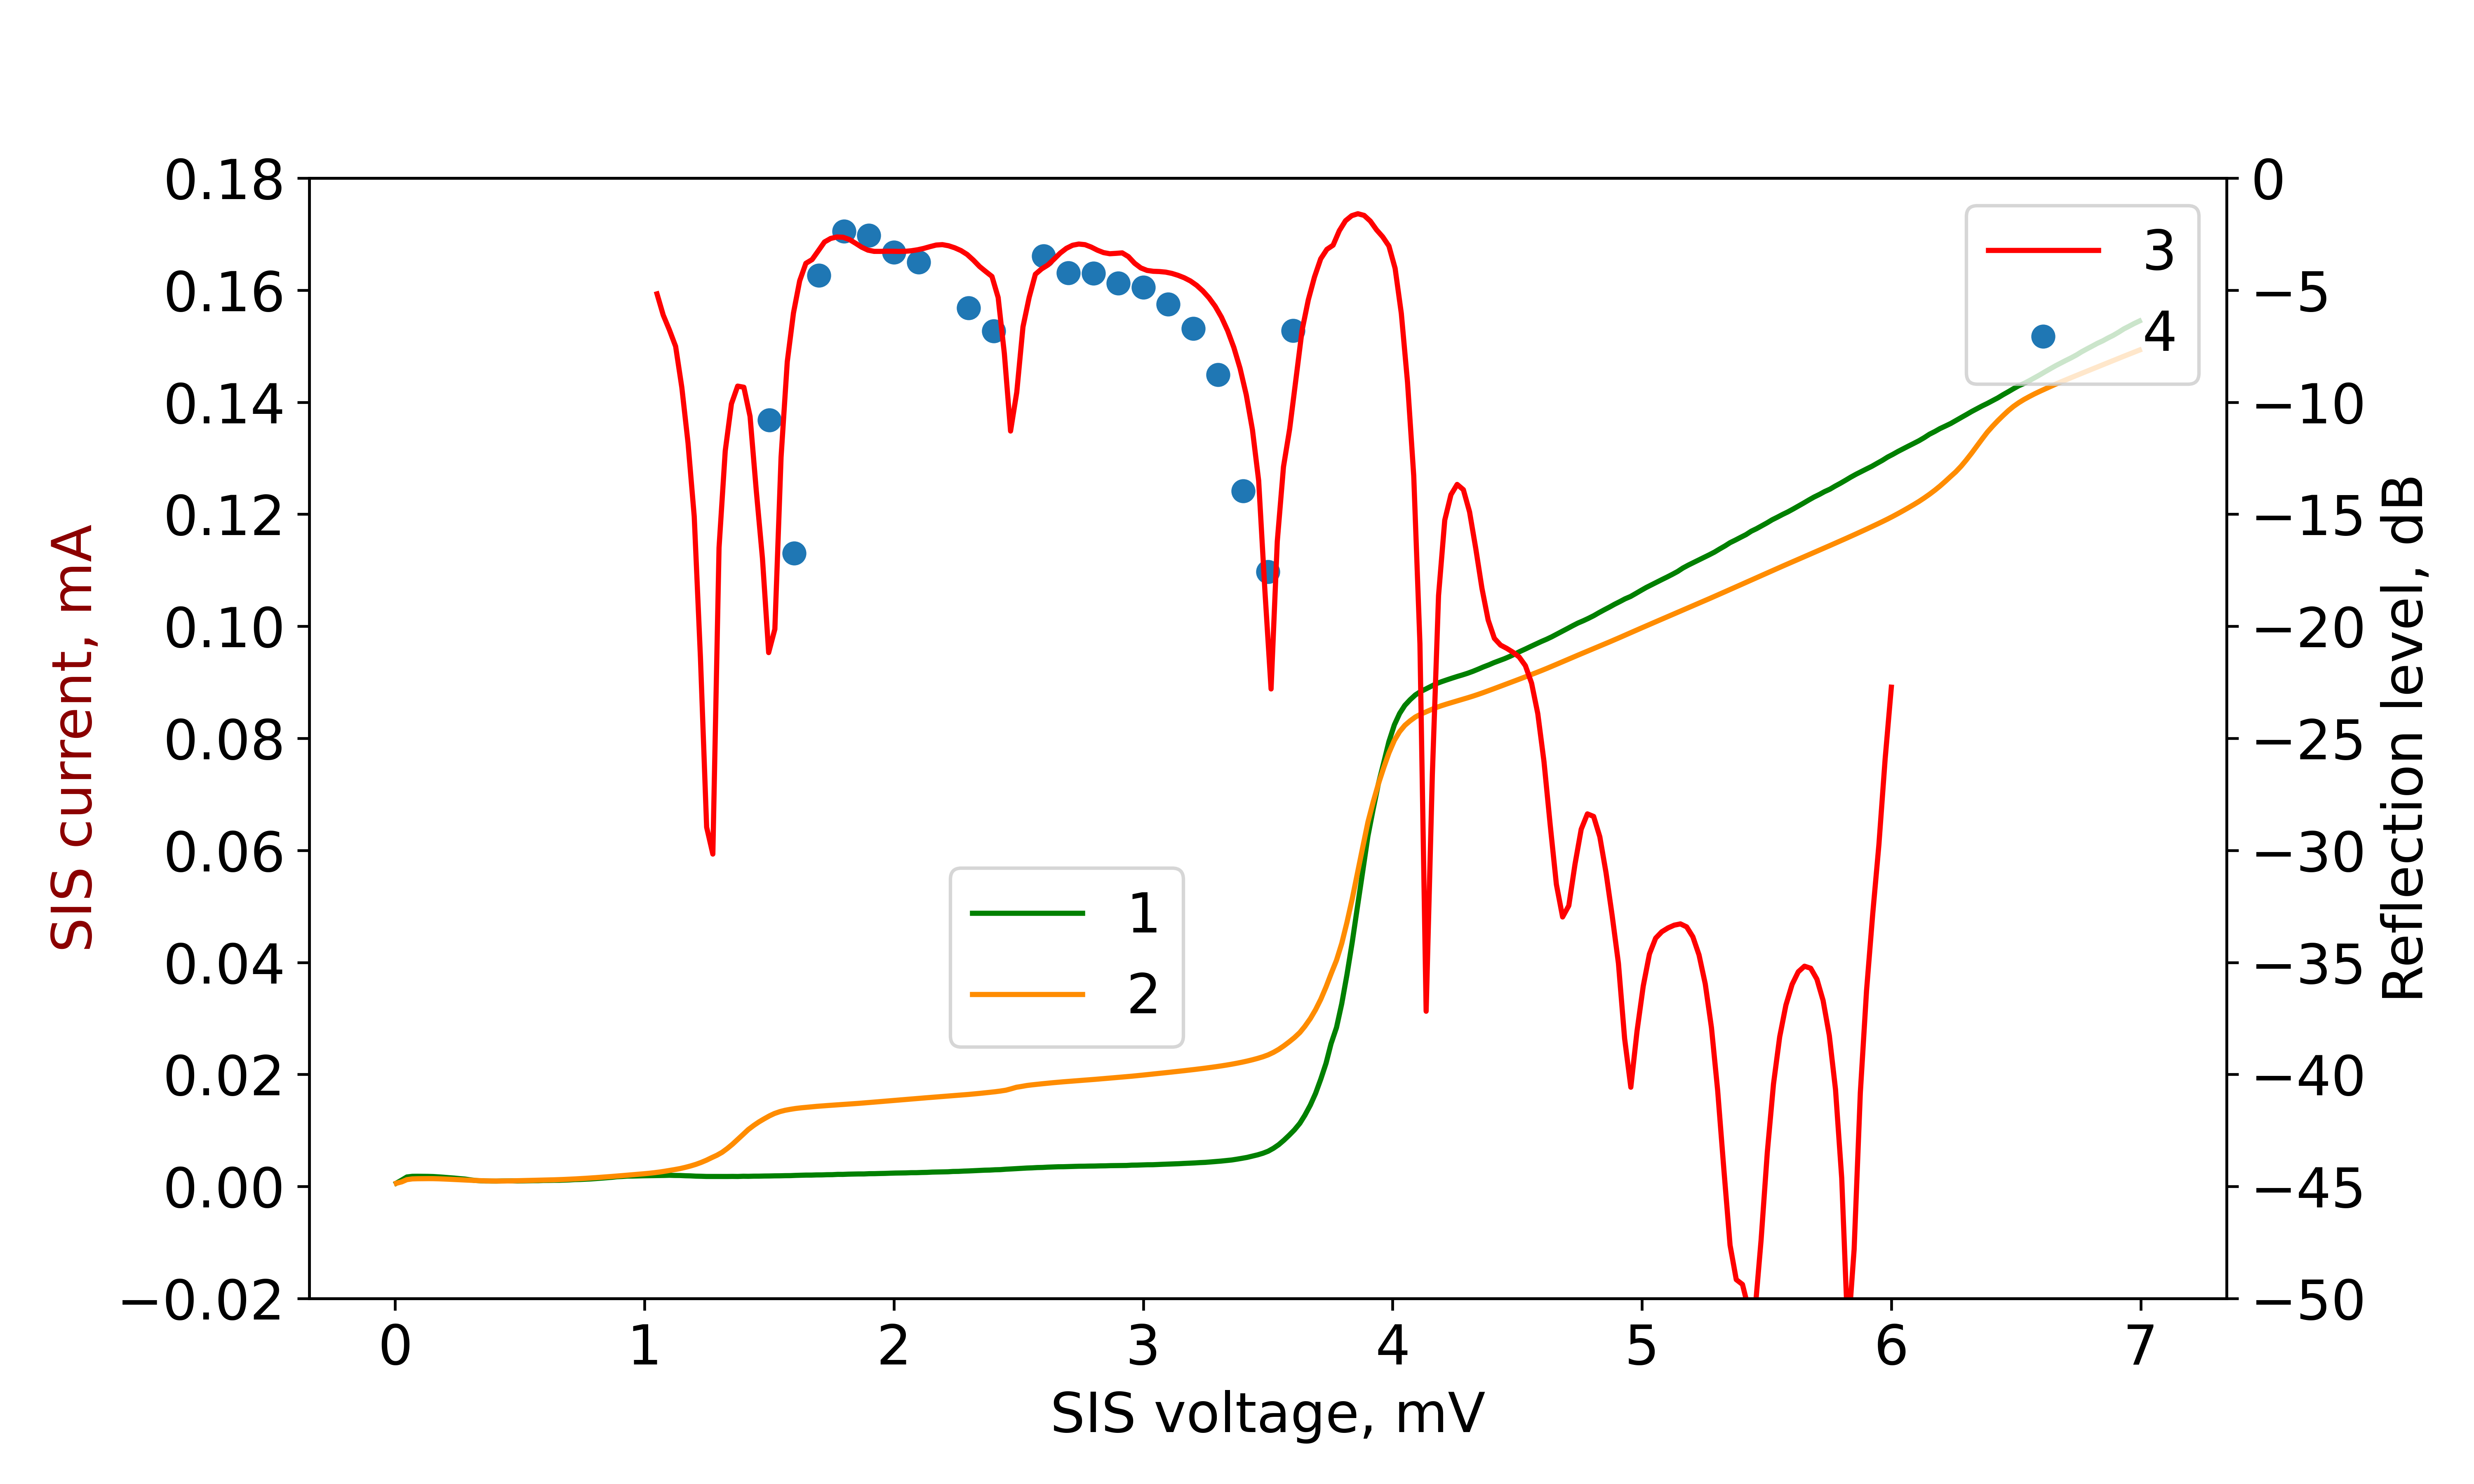
\includegraphics[scale=0.6]{refl.png}
    \caption{ВАХ СИС-смесителя: автономная (№ 1 зеленая кривая), нагруженная сигналом опорного генератора (№ 2 оранжевая кривая). Теоретический расчет отражения (№ 3 красная кривая). Результаты измерений отражения (№ 4 синие точки). ПЧ равна 6 ГГц.}
    \label{pic-refl}
\end{figure}

\begin{figure}[H]
    \centering
    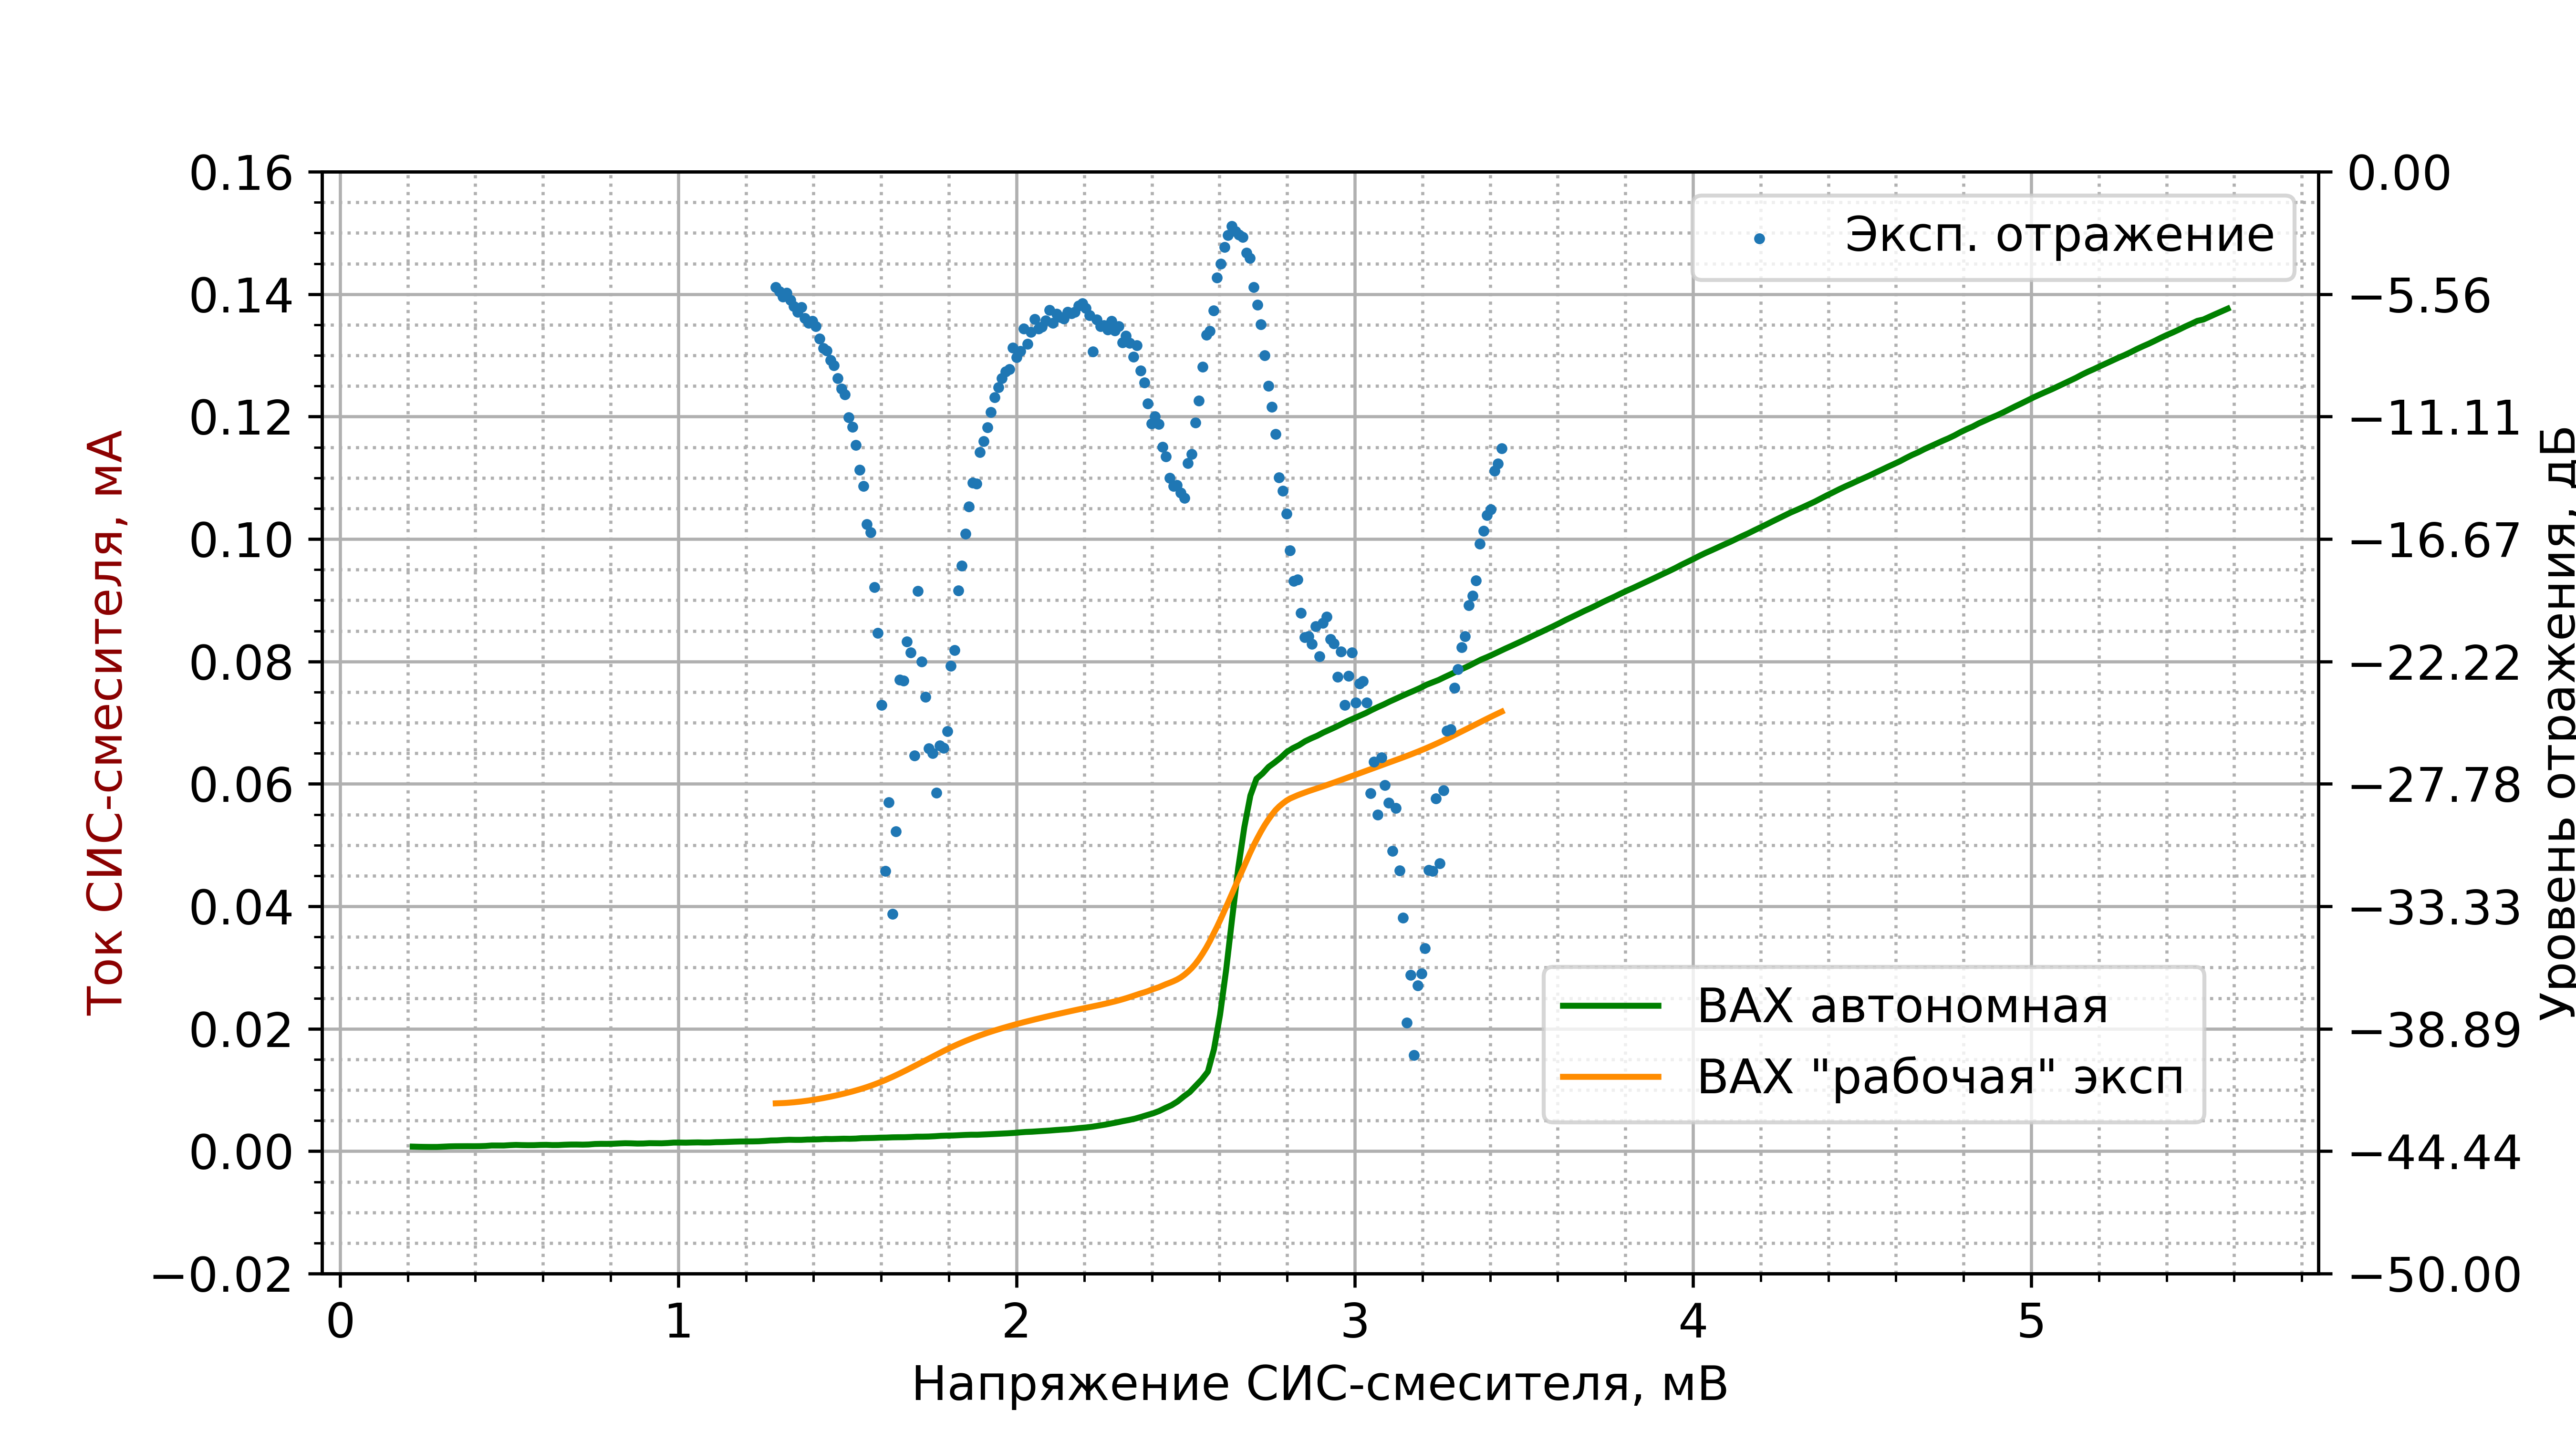
\includegraphics[scale=0.65]{refl2.png}
    \caption{ВАХ <<боевого>> СИС-смесителя: автономная (зеленая кривая), нагруженная сигналом опорного генератора (оранжевая кривая). Результаты измерений отражения (синие точки). ПЧ равна 6 ГГц.}
    \label{pic-refl2}
\end{figure}

\subsubsection{Пик поглощения}

Можно заметить, что при напряжении 3.5 мВ уровень отражения значительно снижается (детально на Рис.\ref{pic-load_imp}). Этот пик поглощения можно объяснить тем, что импеданс СИС-смесителя становится почти равным  импедансу подводящей линии ПЧ, формула (\ref{s11}). Точнее, в этой точке дифференциальное сопротивление СИС-смесителя становится равным действительной компоненте импеданса подводящей линии. Вычислив импеданс СИС-смесителя по формуле (\ref{s11}) мы сможем экспериментально определить импеданс подводящей линии . В данном случае, мы наблюдаем, что  с высокой степенью точности составляет  Ом. На Рис.\ref{pic-load_imp} приведено сравнение экспериментального уровня отражения и теоретического. Важно отметить, что уровень отражения в минимуме определяется модулем разности мнимых компонент импедансов СИС-смесителя и подводящей линии. Отличие глубины пика поглощения в измерении и в расчете позволяет проверить достоверность расчета, а также оценить величину комплексной части импеданса подводящей линии и за счет проведения измерений при различных частотах ПЧ. В нашем случае можно заключить, что мнимая часть импеданса подводящей линии не превышает 2 Ом. Таким образом, предложен и апробирован способ нахождения импеданса подводящей линии, используя особенности ВАХ СИС-смесителя.
В целом, можно заключить, что уровень отражения достаточно высокий и составляет в среднем около -4.5дБ в «рабочем» диапазоне, что вынуждает нас использовать специальные вентили в канале ПЧ в СИС приемниках для минимизации стоячих волн в тракте ПЧ.

\begin{figure}[H]
    \centering
    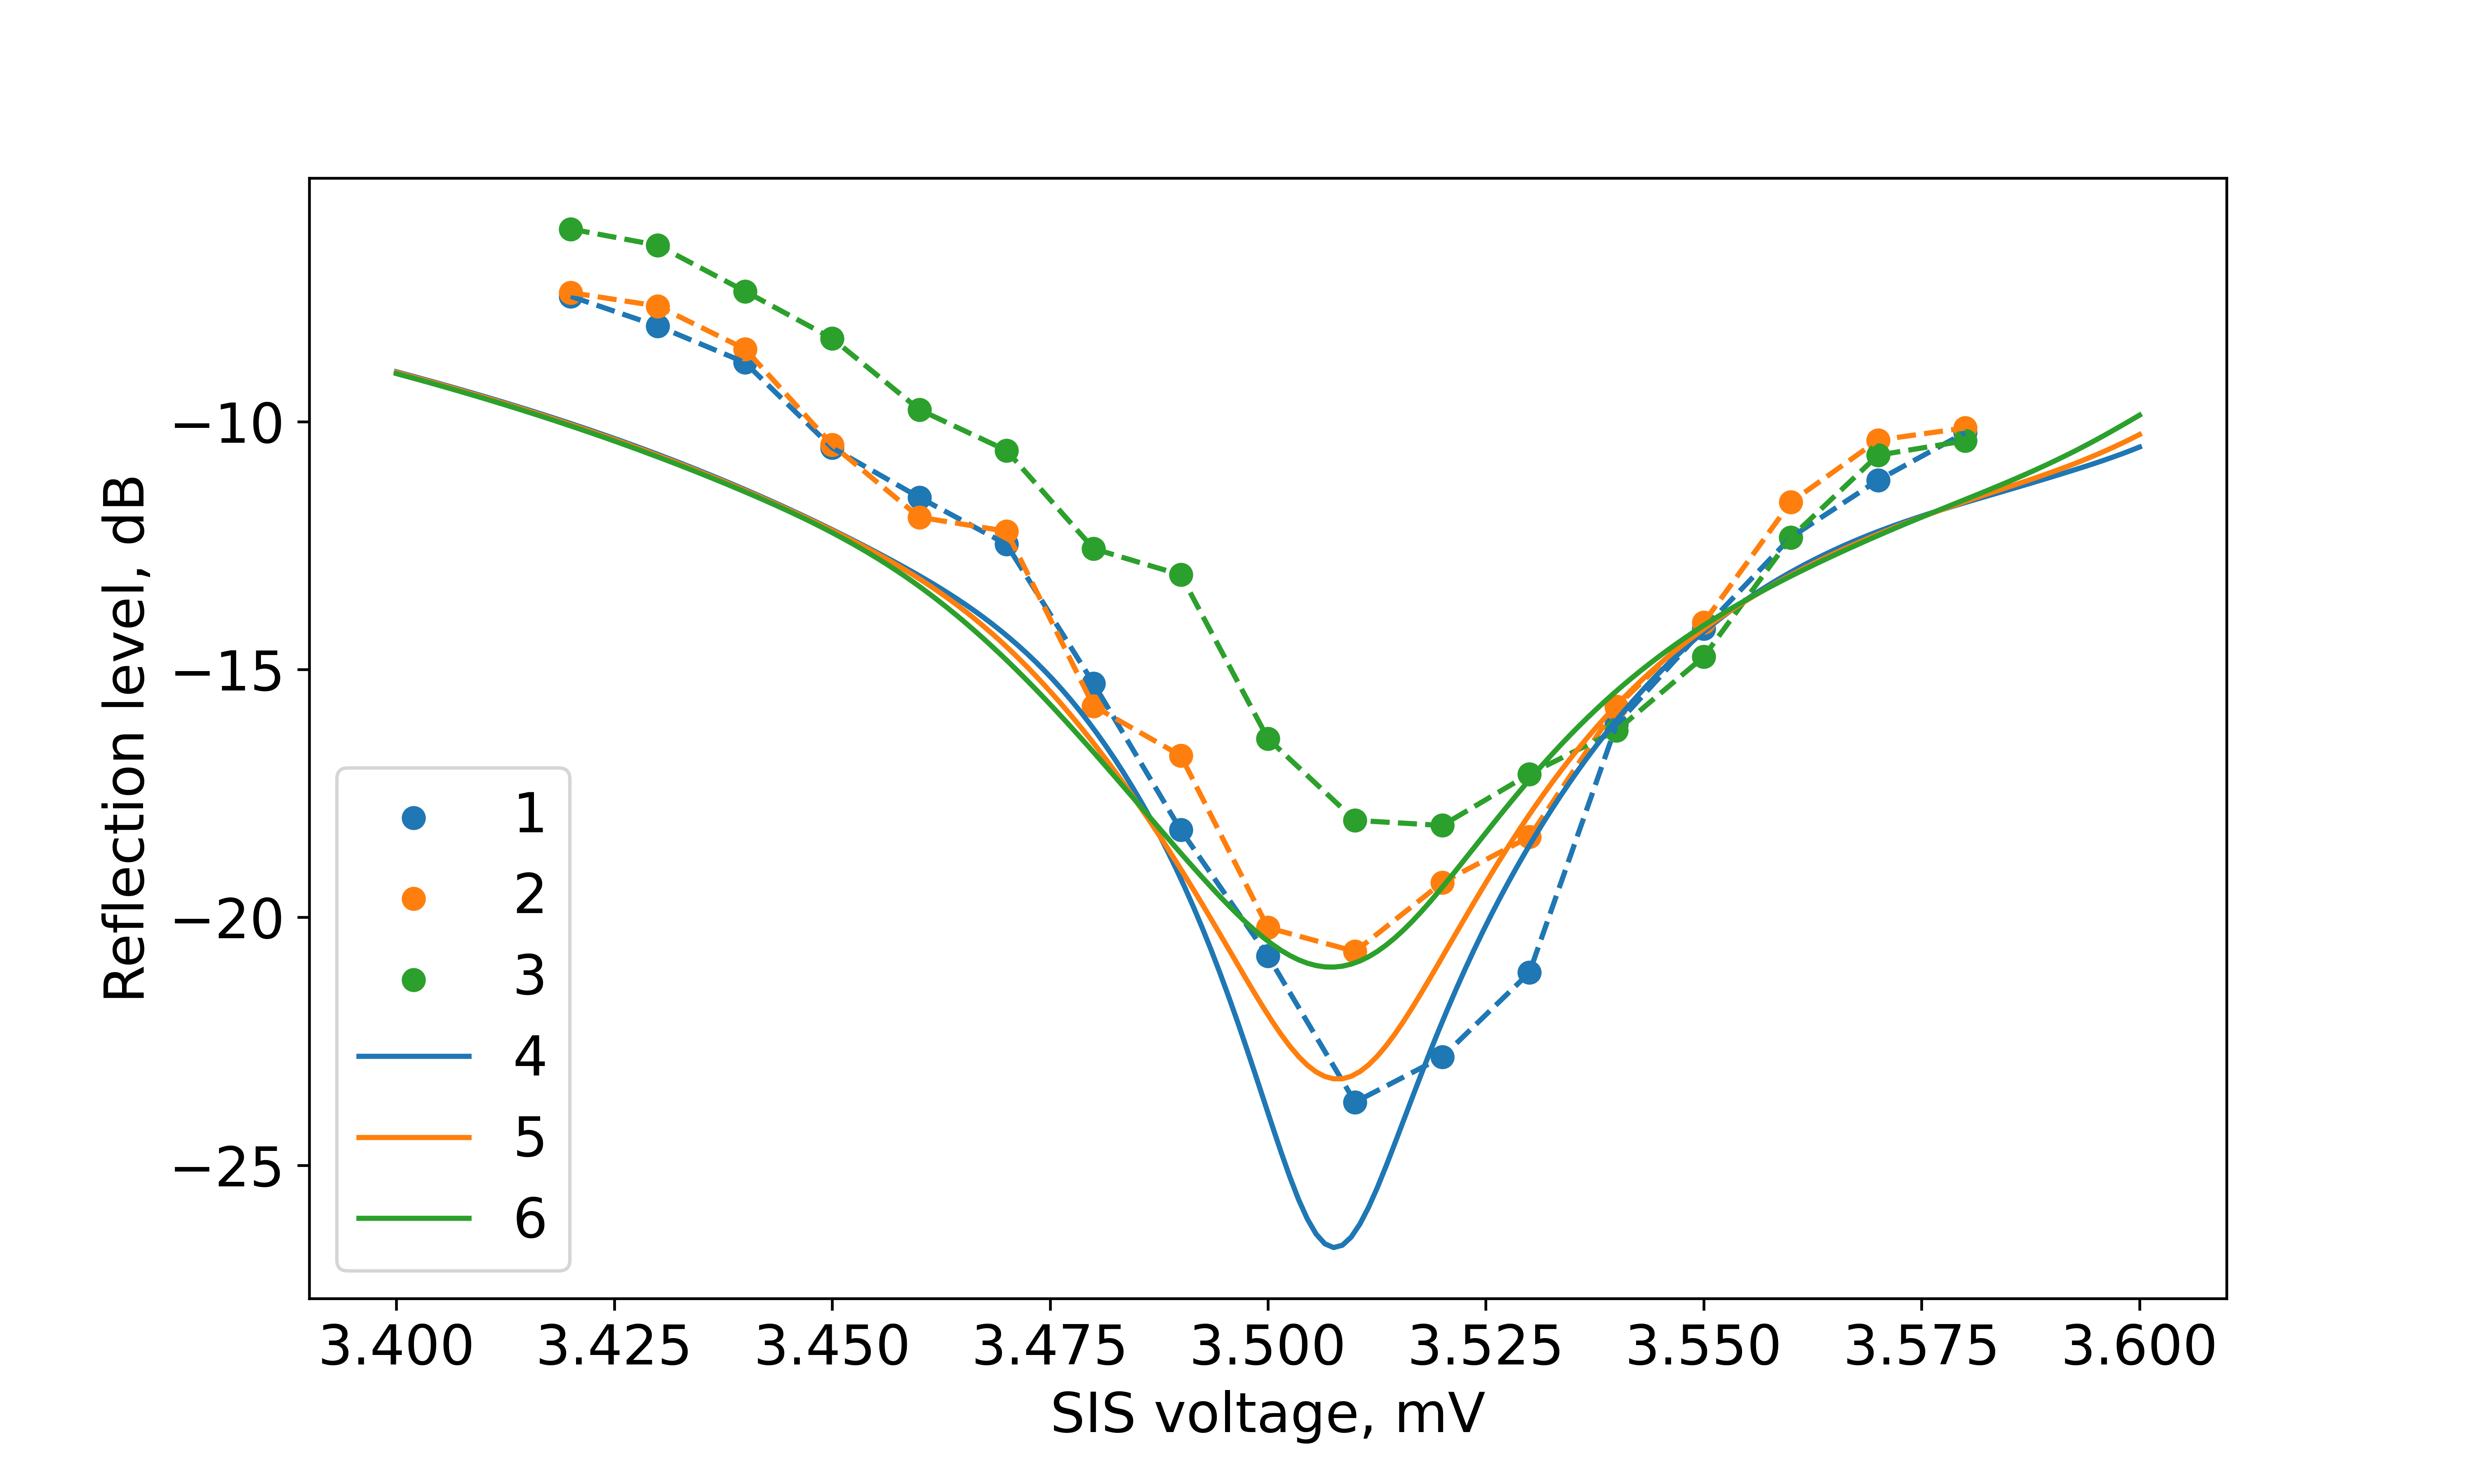
\includegraphics[scale=0.5]{load_imp.png}
    \caption{Уровень отражения в «яме». Точки (№ 1,2,3) - экспериментальный уровень отражения для ПЧ 4,6,8 ГГц соответсвенно; Сплошные кривые (№ 4,5,6) - теоретический расчет уровня отражения для ПЧ 4,6,8 ГГц соответсвенно.}
    \label{pic-load_imp}
\end{figure}


\newpage
\section{Заключение}
Представлен метод экспериментального и теоретического определения ПЧ параметров СИС-перехода. Это позволяет исследовать зависимость уровня отражений от СИС-смесителя по ПЧ выходу от напряжения смещения и от мощности опорного сигнала. Определение параметров самого СИС-перехода совмещенное с моделированием элементов ПЧ канала позволит в будущем рассчитать с высокой точностью ПЧ характеристики самого смесителя, а также всего приёмника сконструированного на его основе. Дополнительная калибровка по пику поглощения при варьировании напряжения смещения позволяет повысить точность измерений, которые хорошо совпадают с теоретическим расчетом. Также представленный код позволяет вычислять импеданс (уровень отражения) по ПЧ СИС-смесителя с учетом импеданса внешней цепи, проводить измерение и калибровку в автоматизированном режиме. \par 

В дальнейшем планируется исследование ПЧ параметров на частотах 4-12 ГГц и выше, а также при варьировании мощности опорного генератора в широком диапазоне.


\newpage
\begin{thebibliography}{12}

\bibitem{Tucker} Tucker J.R., Feldman M.J. Quantum detection at millimeter wavelengths. Rev. Mod. Phys. \textbf{57}, \textit{4}, 1055—1113, DOI:10.1103/RevModPhys.57.1055 (1985)

\bibitem{Belitsky} Belitsky, V., Bylund, M., Desmaris, V., Ermakov, A., Ferm, S.E., Fredrixon, M., Krause, S., Lapkin, I., Meledin, D., Pavolotsky, A. and Rashid, H., ALMA Band 5 receiver cartridge-Design, performance, and commissioning. Astronomy \& Astrophysics, 611, p.A98 (2018)

\bibitem{Chenu} Chenu, J.Y., Navarrini, A., Bortolotti, Y., Butin, G., Fontana, A.L., Mahieu, S., Maier, D., Mattiocco, F., Serres, P., Berton, M. and Garnier, O., The front-end of the NOEMA interferometer. IEEE Transactions on Terahertz Science and Technology, 6(2), 223 (2016)

\bibitem{Hesper} Hesper, R., Khudchenko, A., Baryshev, A.M., Barkhof, J. and Mena, F.P., A high-performance 650-GHz sideband-separating mixer—design and results. IEEE Transactions on Terahertz Science and Technology, 7(6), 686 (2017)

\bibitem{Khudchenko} Khudchenko, A., Hesper, R., Barkhof, J., Mena, F.P. and Baryshev, A.M., September. Comprehensive Description of Sideband Ratio of 2SB SIS Receiver. In 2019 44th International Conference on Infrared, Millimeter, and Terahertz Waves (IRMMW-THz) (pp. 1-2). IEEE.  (2019)

\bibitem{Kooi} Kooi J.W., Advanced Receivers for Submillemeter and Far Infrared Astronomy. Print Partners Ipskamps B.V., Enschede, The Netherlands, ISBN 978-90-367-3653-4 (2008)

\bibitem{Serres} Serres P. et al., The IF Output Impedance of SIS Mixers. IEEE Transactions on Terahertz Science and Technology, \textbf{5}, \textit{1}, 27 (2015)

\bibitem{Barichev} Barichev A.M., Superconductor-Insulator-Superconductor THz Mixer Integrated with a Superconducting Flux-Flow Oscillator. PhD thesis, Delft University of Technology, ISBN 90-9019220-4 (2005)

\bibitem{Garrett} Garrett J.D., A 230 GHz Focal Plane Array Using a Wide IF Bandwidth SIS Receiver. PhD thesis, University of Oxford, (2018)

\bibitem{Shen} Shen T.M., Conversion gain in millimeter wave quasi-particle heterodyne mixers. IEEE J. Quantum Electronics, \textbf{17},  \textit{7}, 1151 (1981)

\bibitem{Walker} Walker B., One-Port VNA Calibration: A Look Under the Hood. Copper Mountain Technologies. \href{https://www.researchgate.net/publication/349533253_One_Port_VNA_Calibration_a_look_under_the_hood}{ResearchGate} (2020)

\bibitem{Rudakov} Rudakov K., Dmitriev P., Baryshev A., Khudchenko A., Hesper R., Koshelets V. Low-Noise Sis Receivers for New Radio-Astronomy Projects. Radiophysics and Quantum Electronics. \textbf{62}. DOI: 10.1007/s11141-020-10001-7. (2020)

\end{thebibliography}


\newpage
\section{Приложение}
Весь код доступен на \href{https://github.com/yarvod/vna_cals}{github.com/yarvod/vna\_cals}
\begin{enumerate}
    \item \textbf{Код расчета импеданса СИС-смесителя; Mixer.py} \par 
    \lstinputlisting{Mixer.py}
    \item \textbf{Код взаимодействия с блоком смещения по напряжению; scpi.py} \par 
    \lstinputlisting{scpi.py}
    \item \textbf{Код взаимодействия с VNA; vna.py} \par 
    \lstinputlisting{vna.py}
\end{enumerate}

\end{document}